\documentclass[a4paper,twocolumn,10pt,fleqn]{book}
\usepackage[american,ngerman]{babel}     %american / ngerman
\usepackage[OT1]{fontenc}       %Silbentrennung
\usepackage[utf8]{inputenc}
%\usepackage[latin1]{inputenc}  %Direkteingabe von Umlauten
\usepackage{tabularx}
\usepackage{multirow}
\usepackage{colortbl}
\usepackage{longtable}
\usepackage{graphicx}
\usepackage{times}       %Erzwingt Typ 1 Schrift (skalierbar, gutes pdf-Output)
\usepackage[round,colon,authoryear]{natbib}      %Fuer Zitate mit \citep, \citet
\usepackage[fleqn]{amsmath}  % für \align-environment (ausgerichtete Gleichungen)
\usepackage{wasysym}  % common symbols (math + text mode), e.g. \permil
\usepackage{fancyhdr} % Customized header/footer
\usepackage{titling}
\usepackage{fink}
\usepackage{listings}
\usepackage{xcolor}
\usepackage{framed}
\usepackage{amsmath}
\usepackage[hyphens,obeyspaces]{url}
\usepackage{datatool}
\usepackage{lscape}


%Unterdrueckung von Hurenkindern und Schusterjungen
\clubpenalty = 10000
\widowpenalty = 10000 \displaywidowpenalty = 10000

% Vertiacal spacing between multi-line equations (e.g. in align env.)
\setlength{\jot}{11pt}

\newcommand{\fmtClassDesc}[1]{\usefont{OT1}{phv}{mc}{n} \fontsize{8pt}{8pt}
  \selectfont #1}

\newcommand{\ECHSEENGINES}{../../../../echse_engines}


  
%%%%%%%%%%%%%%%%%%%%%%%%%%%%%%%%%%%%%%%%%%%%%%%%%%%%%%%%%
%%%%%%%%%%%%%%%%%%%%%% DEFINITIONS %%%%%%%%%%%%%%%%%%%%%%
%%%%%%%%%%%%%%%%%%%%%%%%%%%%%%%%%%%%%%%%%%%%%%%%%%%%%%%%%

%%%%%%%%%%%%%%%%%%%%%%%%%%%%%%%%%%%%%%%%%
% Optionen f�r die PDF-Erstellung 
%
% Achtung: Der Postprocessor dvips muss
%   mit der Option -z ausgef�hrt werden.
%%%%%%%%%%%%%%%%%%%%%%%%%%%%%%%%%%%%%%%%%
\usepackage[ps2pdf]{hyperref}
\usepackage{breakurl}
\definecolor{darkblue}{rgb}{0.2,0.2,0.8}
\hypersetup{%
colorlinks=true,        % Einfaerbung von Verknuepfungen
linkcolor=darkblue,     %Farbe dokumentinterner Links
citecolor=darkblue,     %Farbe dokumentinterner Links
bookmarksopen=false,    % Anzeige aller Ebenen
bookmarksnumbered=true, % Anzeige der Abschnittsnummern
pdfstartpage={1},       % Startseite
breaklinks=true
}

\usepackage[textfont={small,sl},labelfont={small,bf,sl},indention=0cm,singlelinecheck=false]{caption}
\captionsetup[figure]{position=bottom}
\captionsetup[table]{position=top}

%% Here it is: the code that adjusts justification and spacing around caption.
%% http://www.texnik.de/floats/caption.phtml
%\makeatletter
%% This does spacing around caption.
%\setlength{\abovecaptionskip}{0.3cm}
%\setlength{\belowcaptionskip}{0.3cm}
%% This does justification (left) of caption.
%\long\def\@makecaption#1#2{%
%  \vskip\abovecaptionskip
%  \sbox\@tempboxa{#1: #2}%
%  \ifdim \wd\@tempboxa >\hsize
%    #1: #2\par
%  \else
%    \global \@minipagefalse
%    \hb@xt@\hsize{\box\@tempboxa\hfil}%
%  \fi
%  \vskip\belowcaptionskip}
%\makeatother

% These commands are redefined in each chapter
\newcommand{\tabdir}{UNDEFINED}
\newcommand{\figdir}{UNDEFINED}

\newcommand{\tabref}[1]{Table~\ref{#1}}
\newcommand{\tabsref}[1]{Tables~\ref{#1}}
\newcommand{\figref}[1]{Fig.~\ref{#1}}
\newcommand{\figsref}[1]{Figs.~\ref{#1}}
\newcommand{\eqnref}[1]{Eqn.~\ref{#1}}
\newcommand{\eqnsref}[1]{Eqns.~\ref{#1}}
\newcommand{\appref}[1]{Appendix~\ref{#1}}
\newcommand{\secref}[1]{Sec.~\ref{#1}}
\newcommand{\secsref}[1]{Sections~\ref{#1}}
\newcommand{\chapref}[1]{Chap.~\ref{#1}}
\newcommand{\chapsref}[1]{Chapters~\ref{#1}}

\newenvironment{enumeratePacked}{
\begin{enumerate}
  \setlength{\itemsep}{4pt}
  \setlength{\parskip}{0pt}
  \setlength{\parsep}{0pt}
}{\end{enumerate}}

\newenvironment{itemizePacked}{
\begin{itemize}
  \setlength{\itemsep}{4pt}
  \setlength{\parskip}{0pt}
  \setlength{\parsep}{0pt}
}{\end{itemize}}

\newenvironment{descriptionPacked}{
\begin{description}
  \setlength{\itemsep}{4pt}
  \setlength{\parskip}{0pt}
  \setlength{\parsep}{0pt}
}{\end{description}}

% A command to produce an emphasized header on a single line
\newcommand{\desclisthead}[1]{\par\medskip\noindent\textit{\textbf{#1}}\\*\noindent}

% Modifies the format of the label in description environments (boldface --> italic)
\renewcommand{\descriptionlabel}[1]%
         {\hspace{\labelsep}\textit{#1}}

% Description env. with tt-Font label
\newcommand\mydescriptionlabel[1]{\hspace{\labelsep}\texttt{#1}}
\newenvironment{columndef}{%
   \let\descriptionlabel\mydescriptionlabel
   \description
}{%
   \enddescription
}

% An environment for the chapter introduction
\newenvironment{chapterintro}{
\begin{minipage}{0.75\textwidth}\slshape
}{\upshape \end{minipage}\twocolumn}


%%%%%%%%%%%%%%%%%%%%%%%%%%%%%%%%%%%%%%%%%%%%%%%%%%%%%%%%%%%%%%%%%%%%%%%%%%%%%
% COLOR DEFINITIONS
%%%%%%%%%%%%%%%%%%%%%%%%%%%%%%%%%%%%%%%%%%%%%%%%%%%%%%%%%%%%%%%%%%%%%%%%%%%%%

\definecolor{black}{rgb}{0,0,0}
\definecolor{darkgrey}{rgb}{0.2,0.2,0.2}
\definecolor{darkblue}{rgb}{0,0,0.7}
\definecolor{listnumbercolor}{rgb}{0.5,0.5,0.5}
\definecolor{brown}{rgb}{0.5,0.2,0}
\definecolor{magenta}{rgb}{0.7,0,0.4}

\definecolor{lightyellow}{rgb}{1.,1.,0.75}
\definecolor{lightblue}{rgb}{0.95,0.95,1}

%%%%%%%%%%%%%%%%%%%%%%%%%%%%%%%%%%%%%%%%%%%%%%%%%%%%%%%%%%%%%%%%%%%%%%%%%%%%%
% LANGUAGE DEFINITIONS
%%%%%%%%%%%%%%%%%%%%%%%%%%%%%%%%%%%%%%%%%%%%%%%%%%%%%%%%%%%%%%%%%%%%%%%%%%%%%

\lstdefinelanguage{txt}[]{}{%
  morecomment=[l]{\#}
}

%\lstloadlanguages{R}
\lstdefinelanguage{Renhanced}[]{R}{%
  morekeywords={colMeans,colSums,data.frame,dyn.load,dyn.unload,%
    in,is.na,is.null,is.finite,%
    mapply,na.rm,read.table,rep,rowMeans,rowSums,%
    which.max,which.min,write.table},
  deletekeywords={by,case,dir,dt,col,data,file,model,offset,par,sample,t,time},
  otherkeywords={!, \{, \}}, % Makes operators not keywords
  alsoletter={_.\%},
  alsoother={:\$},
  emph=[1]{TRUE,FALSE,NULL,NA,INF},
  morecomment=[is]{\#\#BeginHide}{\#\#EndHide}
}

%%%%%%%%%%%%%%%%%%%%%%%%%%%%%%%%%%%%%%%%%%%%%%%%%%%%%%%%%%%%%%%%%%%%%%%%%%%%%
% GENERIC STYLE DEFINITIONS
%%%%%%%%%%%%%%%%%%%%%%%%%%%%%%%%%%%%%%%%%%%%%%%%%%%%%%%%%%%%%%%%%%%%%%%%%%%%%

\lstdefinestyle{source}{extendedchars=true,
  basicstyle=\color{black}\ttfamily\small,
  commentstyle=\color{darkgrey}\textsl,
  keywordstyle=\color{darkblue}\textbf,
  stringstyle=\color{brown},
  emphstyle=[1]\color{magenta},
  showstringspaces=false,
  framexleftmargin=0mm,
  frame=shadowbox,
  rulesepcolor=\color{darkgrey},
  backgroundcolor=\color{lightblue},
  rulecolor=\color{lightblue},
  fillcolor=\color{lightblue}
%  numbers=left,
%  numberstyle=\color{darkgrey}\ttfamily\tiny,
%  stepnumber=1,
%  numbersep=3mm
}

\lstdefinestyle{data}{extendedchars=true,
  basicstyle=\color{black}\ttfamily\small,
  commentstyle=\color{darkgrey}\textsl,
  keywordstyle=\color{darkblue}\textbf,
  stringstyle=\color{brown},
  emphstyle=[1]\color{magenta},
  showstringspaces=false,
  framexleftmargin=0mm,
  frame=shadowbox,
  rulesepcolor=\color{darkgrey},
  backgroundcolor=\color{lightyellow},
  rulecolor=\color{lightyellow},
  fillcolor=\color{lightyellow}
%  numbers=left,
%  numberstyle=\color{darkgrey}\ttfamily\tiny,
%  stepnumber=1,
%  numbersep=3mm
}

%%%%%%%%%%%%%%%%%%%%%%%%%%%%%%%%%%%%%%%%%%%%%%%%%%%%%%%%%%%%%%%%%%%%%%%%%%%%%
% ACTUALLY USED STYLES
%%%%%%%%%%%%%%%%%%%%%%%%%%%%%%%%%%%%%%%%%%%%%%%%%%%%%%%%%%%%%%%%%%%%%%%%%%%%%

\lstdefinestyle{R}{language=Renhanced,style=source}
\lstdefinestyle{r}{language=Renhanced,style=source}

\lstdefinestyle{C++}{language=C++,style=source}
\lstdefinestyle{c++}{language=C++,style=source}
\lstdefinestyle{cpp}{language=C++,style=source}

\lstdefinestyle{shell}{language=bash,style=source}

\lstdefinestyle{txt}{language=txt,style=data}
\lstdefinestyle{text}{language=txt,style=data}

\hyphenation{ben-thic}
\hyphenation{ben-thal}
\hyphenation{Be-wert-ungs-skala}
\hyphenation{cyano-bac-teria}
\hyphenation{eu-tro-phic}
\hyphenation{eu-tro-phic-ation}
\hyphenation{de-ni-tri-fica-tion}
\hyphenation{dia-tom}
\hyphenation{dia-toms}
\hyphenation{hydro-graph}
\hyphenation{hydro-graphs}
\hyphenation{hypo-rheic}
\hyphenation{hypo-rheal}
\hyphenation{inter-stitial}
\hyphenation{macro-phyte}
\hyphenation{macro-phytes}
\hyphenation{pelagic}
\hyphenation{pelagial}
\hyphenation{phyto-plankton}
\hyphenation{ripa-rian}
\hyphenation{zoo-plankton}


\newcommand{\software}[1]{\texttt{\textbf{#1}}}

\newcommand{\function}[1]{\texttt{#1}}


%%%%%%%%%%%%%%%%%%%%%%%%%%%%%%%%%%%%%%%%%%%%%%%%%%%%%%%%%%%%%%%%%%%%%%%%%%%%%%%%
% MISCELLANEOUS
%%%%%%%%%%%%%%%%%%%%%%%%%%%%%%%%%%%%%%%%%%%%%%%%%%%%%%%%%%%%%%%%%%%%%%%%%%%%%%%%

% Real abbreviations
\newcommand{\ie}{i.~e.}
\newcommand{\eg}{e.~g.}

\newcommand{\first}{\ensuremath{1^{\rm st}}}  %1st
\newcommand{\second}{\ensuremath{2^{\rm nd}}}  %2nd

% Sub- and superscripts ...
\newcommand{\h}[1]{\ensuremath{^{\rm #1}}}  %superscript
\renewcommand{\l}[1]{\ensuremath{_{\rm #1}}}  %subscript
\newcommand{\e}[1]{\ensuremath{\cdot 10^{\rm #1}}}  % produces "*10^{arg}

% Typical math symbols
\newcommand{\deltat}{\ensuremath{\Delta t}}
\newcommand{\deltax}{\ensuremath{\Delta x}}
\newcommand{\average}{\ensuremath{\rm \overline{x}}}

\newcommand{\halflife}{\ensuremath{\tau}}

\newcommand{\tinc}{\texttt{t\_inc}}
\newcommand{\tbeg}{\texttt{t\_beg}}
\newcommand{\tend}{\texttt{t\_end}}



% Locigal values
\newcommand{\true}{\textsc{true}}
\newcommand{\false}{\textsc{false}}



%%%%%%%%%%%%%%%%%%%%%%%%%%%%%%%%%%%%%%%%%%%%%%%%%%%%%%%%%%%%%%%%%%%%%%%%%%%%%%%%
% HYDRO-METEOROLOGICAL VARIABLES
%%%%%%%%%%%%%%%%%%%%%%%%%%%%%%%%%%%%%%%%%%%%%%%%%%%%%%%%%%%%%%%%%%%%%%%%%%%%%%%%

% Basic meteorological variables
\newcommand{\precipIntensity}{\ensuremath{PI}}
\newcommand{\windspeed}{\ensuremath{WS}}
\newcommand{\airtemp}{\ensuremath{TA}}
\newcommand{\airPressure}{\ensuremath{PA}}
\newcommand{\relHumidity}{\ensuremath{RH}}
\newcommand{\solarRadiation}{\ensuremath{SR}}

% Variables related to moisture / humidity
\newcommand{\specHumidity}{\ensuremath{q}}
\newcommand{\specHumiditySurface}{\ensuremath{q_s}}
\newcommand{\vaporPressure}{\ensuremath{e}}
\newcommand{\vaporPressureSurface}{\ensuremath{e_s}}
\newcommand{\satVaporPressure}{\ensuremath{E}}
\newcommand{\satVaporPressureIce}{\ensuremath{E_i}}
\newcommand{\satVaporPressureWater}{\ensuremath{E_w}}

% Other meteorological variables
\newcommand{\cloudFraction}{\ensuremath{FC}}
\newcommand{\dewpointTemperature}{\ensuremath{T_{dew}}}

% Common (unspecific) hydrometeorological variables
\newcommand{\temperature}{\ensuremath{T}}

% Snow variables
\newcommand{\snowWaterEquivalent}{\ensuremath{SWE}}
\newcommand{\snowHeight}{\ensuremath{SH}}
\newcommand{\snowEnergyContent}{\ensuremath{SEC}}
\newcommand{\snowTemperature}{\ensuremath{T_s}}
\newcommand{\snowSurfaceTemperature}{\ensuremath{T_{ss}}}
\newcommand{\snowFractionLiquid}{\ensuremath{SLF}}
\newcommand{\snowRelSaturation}{\ensuremath{RSS}}

%%%%%%%%%%%%%%%%%%%%%%%%%%%%%%%%%%%%%%%%%%%%%%%%%%%%%%%%%%%%%%%%%%%%%%%%%%%%%%%%
% HYDRO-METEOROLOGICAL PROCESS RATES AND RELATED CONVERSION FACTORS
%%%%%%%%%%%%%%%%%%%%%%%%%%%%%%%%%%%%%%%%%%%%%%%%%%%%%%%%%%%%%%%%%%%%%%%%%%%%%%%%

% Energy fluxes
\newcommand{\netRadiationShort}{\ensuremath{R_{netS}}}
\newcommand{\netRadiationLong}{\ensuremath{R_{netL}}}
\newcommand{\heatfluxSens}{\ensuremath{R_{sens}}}
\newcommand{\heatfluxSoil}{\ensuremath{R_{soil}}}

\newcommand{\radLongwaveOut}{\ensuremath{R_{outL}}}
\newcommand{\radLongwaveIn}{\ensuremath{R_{inL}}}
\newcommand{\radLongwaveInClearsky}{\ensuremath{R_{inL,cs}}}
\newcommand{\radLongwaveInClouds}{\ensuremath{R_{inL,cl}}}

\newcommand{\radShortwaveIn}{\ensuremath{R_{inS}}}

% Mass fluxes
\newcommand{\massfluxPrec}{\ensuremath{M_{prec}}}
\newcommand{\massfluxSubl}{\ensuremath{M_{subl}}}
\newcommand{\massfluxFlow}{\ensuremath{M_{flow}}}

% Others
\newcommand{\albedoChangeRate}{\ensuremath{G_{alb}}}

%%%%%%%%%%%%%%%%%%%%%%%%%%%%%%%%%%%%%%%%%%%%%%%%%%%%%%%%%%%%%%%%%%%%%%%%%%%%%%%%
% PHYSICAL CONSTANTS AND CONCEPTUAL PARAMETERS USED IN HYDRO-METEOROLOGY
%%%%%%%%%%%%%%%%%%%%%%%%%%%%%%%%%%%%%%%%%%%%%%%%%%%%%%%%%%%%%%%%%%%%%%%%%%%%%%%%

% Densities
\newcommand{\densityWater}{\ensuremath{\rho_{w}}}
\newcommand{\densityIce}{\ensuremath{\rho_{i}}}
\newcommand{\densityAir}{\ensuremath{\rho_{a}}}
\newcommand{\densitySnow}{\ensuremath{\rho_{snow}}}
\newcommand{\densitySnowDry}{\ensuremath{\rho_{snow,dry}}}
\newcommand{\densitySoil}{\ensuremath{\rho_s}}

% Specific heat capacities
\newcommand{\specHeatWater}{\ensuremath{C_{wat}}}
\newcommand{\specHeatIce}{\ensuremath{C_{ice}}}
\newcommand{\specHeatAir}{\ensuremath{C_{air}}}
\newcommand{\specHeatSoil}{\ensuremath{C_s}}

% Latent heats
\newcommand{\evapHeatWater}{\ensuremath{E_{wat}}}
\newcommand{\evapHeatWaterZero}{\ensuremath{E_{wat,0}}}
\newcommand{\fusionHeatIce}{\ensuremath{H_{ice}}}
\newcommand{\sublimHeatIce}{\ensuremath{E_{ice}}}

% Radiation
\newcommand{\snowAlbedo}{\ensuremath{AS}}
\newcommand{\snowAlbedoMin}{\ensuremath{AS_{min}}}
\newcommand{\snowAlbedoMax}{\ensuremath{AS_{max}}}
\newcommand{\snowAlbedoRng}{\ensuremath{AS_{rng}}}

\newcommand{\stefanBoltzmann}{\ensuremath{\sigma}}
\newcommand{\emissivity}{\ensuremath{\varepsilon}}


% Stoichiometry factors and functions used in the snow model
\newcommand{\stoifacPrecMassToEnergy}{\ensuremath{f_{prec}}}
\newcommand{\stoifacSublMassToEnergy}{\ensuremath{f_{subl}}}
\newcommand{\stoifacFlowMassToEnergy}{\ensuremath{f_{flow}}}

% Various parameters of the snow model
\newcommand{\turbTransCoeff}{\ensuremath{D}}
\newcommand{\airtempRainSnow}{\ensuremath{T_{crit}}}
\newcommand{\soilInteractionDepth}{\ensuremath{D_s}}
\newcommand{\snowRelCapRetent}{\ensuremath{SCR}}
\newcommand{\snowSatHydrCond}{\ensuremath{k_{sat,snow}}}
\newcommand{\snowAlbedoDecrConst}{\ensuremath{k_{AS}}}
\newcommand{\leafAreaIndexFullShadow}{\ensuremath{LAI_{r0}}}

% Evapotranspiration
\newcommand{\etPot}{\ensuremath{et_{pot}}}
\newcommand{\etReal}{\ensuremath{et_{real}}}
\newcommand{\leafAreaIndex}{\ensuremath{LAI}}


%%%%%%%%%%%%%%%%%%%%%%%%%%%%%%%%%%%%%%%%%%%%%%%%%%%%%%%%%%%%%%%%%%%%%%%%%%%%%%%%
% CONSTANTS AND VARIABLES RELATED TO RUNOFF GENERATION AND -CONCENTRATION
%%%%%%%%%%%%%%%%%%%%%%%%%%%%%%%%%%%%%%%%%%%%%%%%%%%%%%%%%%%%%%%%%%%%%%%%%%%%%%%%

\newcommand{\soilWaterContent}{\ensuremath{\theta}}
\newcommand{\soilWaterContentMax}{\ensuremath{\theta_{max}}}

\newcommand{\relSat}{\ensuremath{S}}
\newcommand{\relSatInter}{\ensuremath{S_{int}}}
\newcommand{\relSatBase}{\ensuremath{S_{base}}}


\newcommand{\heightRunoffDirect}{\ensuremath{h_{d}}}

\newcommand{\rateRunoffSurf}{\ensuremath{r_{surf}}}
\newcommand{\rateRunoffPref}{\ensuremath{r_{pref}}}
\newcommand{\rateRunoffInter}{\ensuremath{r_{int}}}
\newcommand{\rateRunoffBase}{\ensuremath{r_{base}}}
\newcommand{\rateEvapotransp}{\ensuremath{r_{evap}}}
\newcommand{\rateSnowMelt}{\ensuremath{r_{melt}}}

\newcommand{\soilDepth}{\ensuremath{D}}
\newcommand{\satFrac}{\ensuremath{f_{sat}}}
\newcommand{\expSatFrac}{\ensuremath{{\beta}}}

\newcommand{\thresholdSurf}{\ensuremath{{thr_{surf}}}}

\newcommand{\rateWaterSupply}{\ensuremath{WS}}

\newcommand{\expInter}{\ensuremath{{E_{int}}}}
\newcommand{\expBase}{\ensuremath{{E_{base}}}}

\newcommand{\facInter}{\ensuremath{{b_{int}}}}
\newcommand{\facBase}{\ensuremath{{b_{base}}}}

\newcommand{\strSurf}{\ensuremath{{S_{surf}}}}
\newcommand{\strPref}{\ensuremath{{S_{pref}}}}
\newcommand{\strInter}{\ensuremath{{S_{inter}}}}
\newcommand{\strBase}{\ensuremath{{S_{base}}}}

\newcommand{\concTimeIndex}{\ensuremath{{CTI}}}

\newcommand{\satHydrCond}{\ensuremath{k_{f}}}



% IMPORTANT PHYSICAL UNITS

% Time
\newcommand{\persec}{s\ensuremath{^{-1}}}
\newcommand{\perday}{d\ensuremath{^{-1}}}

% Length
\newcommand{\perm}{m\ensuremath{^{-1}}}
\newcommand{\perdm}{dm\ensuremath{^{-1}}}
\newcommand{\percm}{cm\ensuremath{^{-1}}}
\newcommand{\permm}{mm\ensuremath{^{-1}}}

% Area
\newcommand{\sqkm}{km\ensuremath{^{2}}}
\newcommand{\sqm}{m\ensuremath{^{2}}}
\newcommand{\sqdm}{dm\ensuremath{^{2}}}
\newcommand{\sqcm}{cm\ensuremath{^{2}}}
\newcommand{\sqmm}{mm\ensuremath{^{2}}}

\newcommand{\persqm}{m\ensuremath{^{-2}}}
\newcommand{\persqdm}{dm\ensuremath{^{-2}}}
\newcommand{\persqcm}{cm\ensuremath{^{-2}}}
\newcommand{\persqmm}{mm\ensuremath{^{-2}}}

% Volume
\newcommand{\cbm}{m\ensuremath{^{3}}}
\newcommand{\cbdm}{dm\ensuremath{^{3}}}
\newcommand{\cbcm}{cm\ensuremath{^{3}}}
\newcommand{\cbmm}{mm\ensuremath{^{3}}}

\newcommand{\percbm}{m\ensuremath{^{-3}}}
\newcommand{\percbdm}{dm\ensuremath{^{-3}}}
\newcommand{\percbcm}{cm\ensuremath{^{-3}}}
\newcommand{\percbmm}{mm\ensuremath{^{-3}}}
\newcommand{\perlitre}{l\ensuremath{^{-1}}}

% Mass
\newcommand{\perkg}{kg\ensuremath{^{-1}}}
\newcommand{\perg}{g\ensuremath{^{-1}}}
\newcommand{\permg}{mg\ensuremath{^{-1}}}

% Flow
\newcommand{\cbms}{\cbm~\persec}

% Temperature
\newcommand{\celsius}{\ensuremath{^\circ}C}

\definecolor{shadecolor}{rgb}{0.9,0.9,0.9}


\addtolength{\evensidemargin}{-1cm}
\addtolength{\oddsidemargin}{+1cm}

\setcounter{tocdepth}{2}     % Numbers up to 0.0.0 in TOC     (chapter= 0, section= 1, subsection= 2 ...)
\setcounter{secnumdepth}{3}  % Numbers up to 0.0.0.0 in text  (chapter= 0, section= 1, subsection= 2 ...)

\arrayrulecolor{black}

\begin{document}

%%%%%%%%%%%%%%%%%%%%%%%%%%%%%%%%%%%%%%%%%%%%%%%%%%%%%%%%%
%%%%%%%%%%%%%%%%%%%%%% TITLE PAGES %%%%%%%%%%%%%%%%%%%%%%
%%%%%%%%%%%%%%%%%%%%%%%%%%%%%%%%%%%%%%%%%%%%%%%%%%%%%%%%%

\selectlanguage{american}
\pagestyle{empty}
\onecolumn

\begin{center}
  \vspace*{5cm}
  \LARGE
  \textbf{Eco-Hydrological Simulation Environment \\ (\software{echse})} \\
  \vspace*{1.2cm}
  Documentation of model engines \\
  \vspace*{2.0cm}
  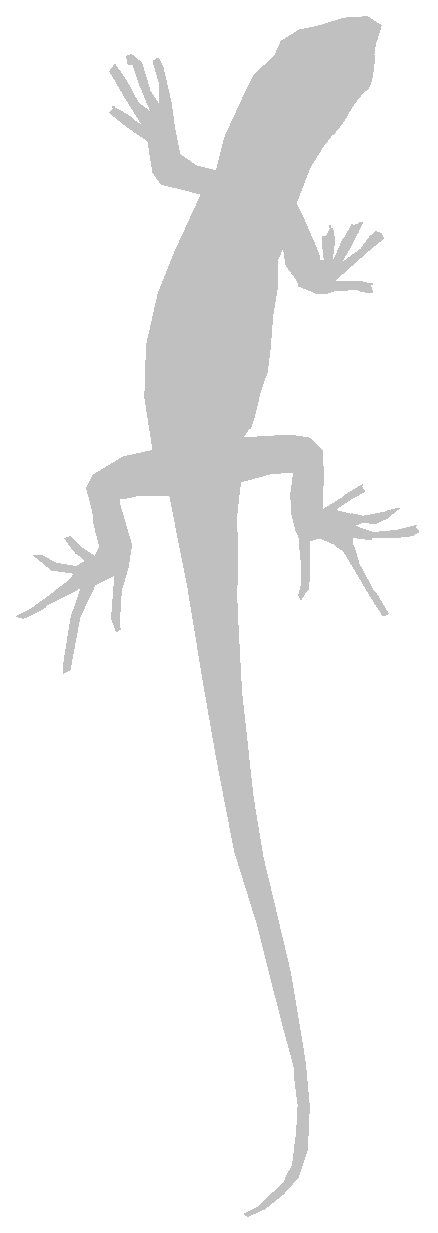
\includegraphics[width=0.1\textwidth,angle=270]{../../_common/fig/logo.eps}
\end{center}

\cleardoublepage

\vspace*{14cm}
\begin{tabular}{ll}
Author      & David Kneis \\
Affiliation & Institute of Earth and Environmental Sciences \\
            & Geo-Ecology Section, \\
            & University of Potsdam, Germany \\
Contact     & david.kneis@uni-potsdam.de \\
            & \\
Project     & PROGRESS \\
Sub-project & D2.2 \\
Funding     & German Ministry of Education and Research (BMBF) \\
            & \\
Last update & \today{} \\
\end{tabular}

\cleardoublepage

%%%%%%%%%%%%%%%%%%%%%%%%%%%%%%%%%%%%%%%%%%%%%%%%%%%%%%%%%%
%%%%%%%%%%%%%%%%%%%%%% Page style   %%%%%%%%%%%%%%%%%%%%%%
%%%%%%%%%%%%%%%%%%%%%%%%%%%%%%%%%%%%%%%%%%%%%%%%%%%%%%%%%%

%%% Begin Fancy Header Settings
\pagestyle{fancy}                       % Sets fancy header and footer
\fancyfoot{}                            % Delete current footer settings
\renewcommand{\chaptermark}[1]{         % Lower Case Chapter marker style
  \markboth{\chaptername\ \thechapter\ \hspace{0.5cm} #1}{}}
\renewcommand{\sectionmark}[1]{         % Lower case Section marker style
  \markright{\thesection\ \hspace{0.5cm} #1}}
\fancyhead[LE,RO]{\bfseries\thepage}    % Page number (boldface) in left on even pages and right on odd pages
\fancyhead[RE]{\bfseries\leftmark}      % Chapter in the right on even pages
\fancyhead[LO]{\bfseries\rightmark}     % Section in the left on odd pages
\renewcommand{\headrulewidth}{0.3pt}    % Width of head rule %%% Clear Header
%% End Fancy Header Settings

%%%%%%%%%%%%%%%%%%%%%%%%%%%%%%%%%%%%%%%%%%%%%%%%%%%%%%%%%%
%%%%%%%%%%%%%%%%%%%%%% TOC          %%%%%%%%%%%%%%%%%%%%%%
%%%%%%%%%%%%%%%%%%%%%%%%%%%%%%%%%%%%%%%%%%%%%%%%%%%%%%%%%%

%% Begin TOC Settings
\pdfbookmark[1]{\contentsname}{toc}
\fancyhead[LE,RO]{\bfseries\thepage}
\fancyhead[RE]{\bfseries Contents}
\fancyhead[LO]{\bfseries Contents}
\tableofcontents
%% End TOC Settings

%%%%%%%%%%%%%%%%%%%%%%%%%%%%%%%%%%%%%%%%%%%%%%%%%%%%%%%%%%
%%%%%%%%%%%%%%%%%%%%%% THE CHAPTERS %%%%%%%%%%%%%%%%%%%%%%
%%%%%%%%%%%%%%%%%%%%%%%%%%%%%%%%%%%%%%%%%%%%%%%%%%%%%%%%%%

% Reestablish header
\fancyhead[LE,RO]{\bfseries\thepage}    % Page number (boldface) in left on even pages and right on odd pages
\fancyhead[RE]{\bfseries\leftmark}      % Chapter in the right on even pages
\fancyhead[LO]{\bfseries\rightmark}     % Section in the left on odd pages


%%%%% Chapter sources

\onecolumn
\chapter{Introduction} \label{chap:intro}
\renewcommand{\tabdir}{chapters/intro/tab}
\renewcommand{\figdir}{chapters/intro/fig}

\section{The \software{echse} simulation environment} \label{sec:intro_idea}

The idea of a \emph{simulation environment}\index{simulation environment}\index{modeling framework|see{simulation environment}}\index{generic model|see{simulation environment}} is to provide a tool which can be used to simulate different systems and/or processes in a single unified software environment. Terms sometimes used more or less synonymously are \emph{modeling framework}, \emph{generic model} or \emph{open structure} model. Examples of existing modeling frameworks in the field of earth and environmental sciences include the \emph{Object Modeling System} \citep{Ahuja2005} and the \emph{Earth System Modeling Framework} \citep{Hill2004}. Examples from the field of water quality modeling include, for example, \emph{AQUASIM} \citep{Reichert1998}, the biogeochemical reactions network simulator BRNS \citep{Regnier2002, Thullner2005}, and the \emph{ECO Lab} software \citep{DHI2006}.

The benefit of a modeling framework usually emerges in situations, where
\begin{itemize}
  \item new models have to be developed in short time.
  \item a preliminary model has to be build and later improvement (possibly by different staff) is planned.
  \item alternative model structures are to be compared (to find an optimum structure or to learn about structural uncertainty).
  \item different people are involved in collaborative model development.
  \item a larger number of individual models must be used and a common (user) interface for all models is required (in operational forecasting, for example).
\end{itemize}

A basic characteristics of a modeling framework is the flexibility to simulate \emph{objects} of different \emph{classes} \footnote{An approximate synonym is \emph{types}.}. Typically, the features of a class, which include \emph{data} and \emph{methods} \footnote{An approximate synonym is \emph{functions}.} are declared/defined by the developer of a specific model for a specific purpose. In contrast to that, the generic core of the modeling framework represents the static part of the software, providing the basic infrastructure for all models (\figref{fig:intro-modelingFramework}).

\begin{figure}
  \centering
  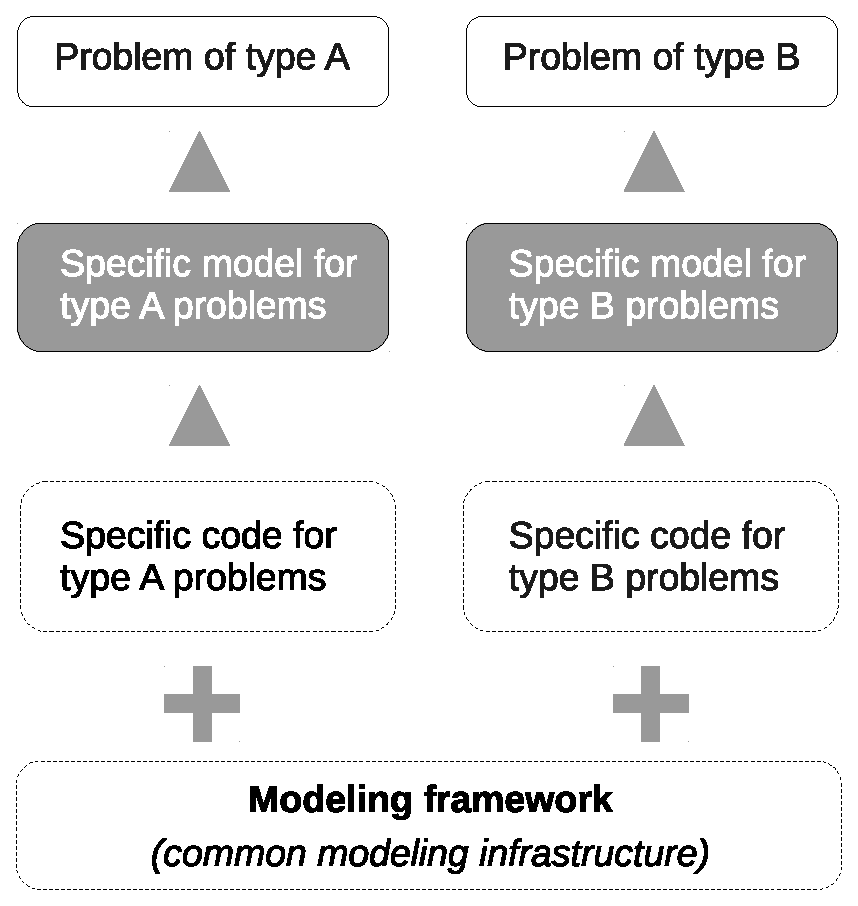
\includegraphics[width=0.9\columnwidth]{\figdir/modelingFramework.eps}
  \caption{Basic idea of a modeling framework. \label{fig:intro-modelingFramework}}
\end{figure}

The \software{echse}\index{\software{echse}} is intended to be a lightweight, simple to use modeling framework, being applicable to many (but not all) simulation problems, arising in the field of (eco)-hydrology. Details on potentials and limits are summarized in \secref{sec:intro_potentials-limits} and discussed in more detail in \chapref{chap:concept}.

It is important to understand that the \software{echse} simulation environment actually consists of two parts:
\begin{description}
  \item [The generic model core] This is a collection of source files. These files provide the common modeling intrastructure shown at the bottom of \figref{fig:intro-modelingFramework}.
  \item [The code generator] This is a software (currently implemented in R) to generate a large part of the \emph{application-specific} source code from basic information provided by the model developer. The generated source code is guaranteed to be compatible with the source code of the generic model core.
\end{description}

In order to create a specific model (grey boxes in \figref{fig:intro-modelingFramework}), the model developer finally has to complement the generated source code by implementing a set of methods (functions) with a simple, well defined interface. Only at this step, source code has to be written manually.

\section{Potential uses and limits} \label{sec:intro_potentials-limits}

Since the potential model applications in the field of eco-hydrology are so diverse, there is (and there cannot be) a modeling framework which is equally suitable for all those applications. Consequently, a 'good' modeling framework is usually one that is specialized on a certain range of applications (as opposed to a 'normal' model, that is specialized on a certain application alone).

The \software{echse} has been developed in the context of hydrological catchment modeling and water quality modeling. Therefore, this modeling framework is particularly specialized on
\begin{itemize}
  \item the simulation of a collection of objects representing instances of different classes (\eg{} catchments, river sections, lakes, etc.).
  \item the simulation of object interactions that are mostly of the \emph{feed-forward} type, \ie{} the simulated flow of mass, energy, or information is mostly unidirectional. \emph{Feedbacks}, \ie{} two-way interations between objects, may also be simulated but there are currently limitations with respect to the accuracy of results.
\end{itemize}

The current version of the \software{echse} is \emph{not} recommended for building models that
\begin{itemize}
  \item are dominated by feedback interactions between the simulated objects. That is, for example, the case in ground water or hydrodynamic modeling, where \emph{partial differential equations} (PDE) have to be solved. The concept of the \software{echse} currently does not support high-accuracy solutions of PDE.
  \item consist of a single object only. Simualting a single object is not a practical problem, but the use of other modeling tools may simply be more efficient.
\end{itemize}

\section{Required user skills} \label{sec:intro_skills}

\subsection{Use of existing models} \label{sec:intro_skills-use}

The skills required for using an existing model built with the \software{echse} are the same as for any other dynamic system model. You basically need to
\begin{itemize}
  \item understand the characteristics of the implemented classes (from a documentation of the specific model).
  \item know which input files are required (see \chapref{chap:input}).
  \item be able to create all input files. This can be done manually (for small projects only), by writing skripts (for example using R, Matlab, Python, etc.), and/or by using other programs such as spreadsheet software, geographical information systems, or data bases.
  \item understand the limits of the implemented model with respect to your specific application.
\end{itemize}

\subsection{Development of models} \label{sec:intro_skills-dev}

As with all modeling frameworks, the \software{echse} aims at reducing the effort for building new models and for changing/extending existing ones. Thus, you don't need to be a professional code writer. However, to successfully create or modify models, you should
\begin{itemize}
  \item understand the meaning of the terms 'class' and 'object' (see any introduction on object-oriented programming),
  \item know the different features of a class supported by \software{echse} and understand the meaning of the classes' 'simulate' methods (see \chapref{chap:concept}),
  \item have basic knowledge of ordinary differential equations and their use in the simulation of dynamic systems,
  \item be able to program simple algorithms in any language,
  \item be willing to get familiar with the most basic elements of C++ (basic data types, operators, and flow-control) or find someone who will translate (or wrap) your code if written in another language.
\end{itemize}


\twocolumn
\part{Hydrological model engines} \label{part:modelEngines}
\chapter{Model engine \software{hypsoRR}} \label{chap:hypsoRR}
\renewcommand{\tabdir}{chapters/part_modelEngines/hypsoRR/tab}
\renewcommand{\figdir}{chapters/part_modelEngines/hypsoRR/fig}

\section{Basic facts}
The \software{hypsoRR} model engine was designed for the purpose of flood forecasting, and the verification of ensemble-based flood forecasts in particular.
\begin{itemize}
  \item It is hydrologocal catchment model engine that simulates all major processes of the hydrological cycle.
  \item It is a rather simple, conceptual model engine to allow for fast computations. This is important in operational applications, especially when dealing with ensembles.
  \item The data requirements are adapted to the situation in Germany, where observation data for all major meteorological variables are typically available. However, the concept was also sucessfully applied to basins in Asia and Africa. The full set of variables is required only if snow accumulation/melt is relevant.
  \item Many concepts are copied from LARSIM \citep{Ludwig2006} which is the hydrological model engine currently used for operational forecasting in SW Germany. \software{hypsoRR} can use most of LARSIM's input data, namely the information in tape12, tape35, etc.
\end{itemize}

\section{Classes}
The \software{hypsoRR} model engine currently comprises the classes listes in \tabref{tab:hypsoRR:classes}.

\begin{table}[h]
  \caption{Classes of the \software{hypsoRR} model engine. \label{tab:hypsoRR:classes}}
\begin{tabular}{ll}
  \hline
  Class & Details to be found at \\
  \hline
  Sub-basin & \secref{sec:classes:catchmod:subbasin-default} \\
  Reach  & \secref{sec:classes:catchmod:reach-default} \\
  Minireach & \secref{sec:classes:catchmod:minireach} \\
  Node classes & \secref{sec:classes:catchmod:nodes} \\  
  Lake & \secref{sec:classes:catchmod:lake} \\
  Gage & \secref{sec:classes:catchmod:gage} \\
  Rain gage & \secref{sec:classes:catchmod:raingage} \\
  External inflow & \secref{sec:classes:catchmod:ext-inflow} \\
  \hline
\end{tabular}
\end{table}

\section{Selected applications}
As of March 2014, \software{hypsoRR} was set-up and calibrated for the river basins listes in \tabref{tab:hypsoRR:applications}.

\begin{table}[h]
  \caption{Applications of the \software{hypsoRR} model engine. \label{tab:hypsoRR:applications}}
  \begin{tabular}{lll}
  \hline
  Basin/Gage & Country & \sqkm{} \\
  \hline
  Wilde Weißeritz / Ammelsdorf & Germany & 70 \\
  Rheraya & Morocco & 220 \\
  Marikina & Philippines & 570 \\
  Neckar / Kirchtellinsfurt & Germany & 2317 \\
  Mahanadi / Mundali & India & 135000 \\
  \hline
  \end{tabular}  
\end{table}


\onecolumn
\part{Classes} \label{part:classes}
\chapter{Classes for hydrological catchment modeling} \label{chap:classes:catchmod}

%NOTE: This code is required by the datatool package to make the reading of TAB-separated text files actually work
\catcode`\^^I=12 %
\DTLsetseparator{	}%

% Generate a long table listing all data members
%
% Arg 1: A name for the data base (e.g. use the class' name)
% Arg 2: The data file listing the members
% Arg 3: The table caption
% Arg 4: The label string
\newcommand{\tableOfMembers}[4]{%
\DTLloadrawdb{#1}{#2}
%\begin{landscape}
\begin{center}
\begin{longtable}{llll}
%\begin{tabular}{llll} \\
\caption{#3 \label{#4}} \\
\hline
\fmtClassDesc\bfseries Type & \fmtClassDesc\bfseries Name & \fmtClassDesc\bfseries Description & \fmtClassDesc\bfseries Unit\\
\hline
\endfirsthead
\multicolumn{4}{c}%
{\tablename\ \thetable\ -- \textit{Continued from previous page}} \\
\hline
\fmtClassDesc\bfseries Type & \fmtClassDesc\bfseries Name & \fmtClassDesc\bfseries Description & \fmtClassDesc\bfseries Unit\\
\hline
\endhead
\hline \multicolumn{4}{r}{\textit{Continued on next page}} \\
\endfoot
\hline
\endlastfoot
\DTLforeach{#1}
{\membertype=type,\membername=name,\memberdescr=description,\memberunit=unit}
{%
  \DTLiffirstrow{}{\\}%
  \fmtClassDesc \membertype & \fmtClassDesc \membername & \fmtClassDesc \memberdescr & \fmtClassDesc \memberunit%
}%
\end{longtable}
%\end{tabular}
\end{center}
}

%%%%%%%%%%%%%%%%%%%%%%%%%%%%%%%%%%%%%%%%%%%%%%%%%%%%%%%%%%%%%%%%%%%%%%%%%%%%%%%%%%%%%%%%%%%%%%
%%%%%%%%%%%%%%%%%%%%%%%%%%%%%%%%%%%%%%%%%%%%%%%%%%%%%%%%%%%%%%%%%%%%%%%%%%%%%%%%%%%%%%%%%%%%%%

\section{Default sub-basin class} \label{sec:classes:catchmod:subbasin-default}

\subsection{Simulated processes} \label{sec:classes:catchmod:subbasin-default:processes}
The class simulates the processes listed in \tabref{tab:classes:catchmod:subbasin-default:processes}.

\begin{table}
  \caption{Considered processes in the default sub-basin class. \label{tab:classes:catchmod:subbasin-default:processes}}
\begin{tabular}{|p{0.28\textwidth}p{0.7\textwidth}|} \hline
  \rowcolor[gray]{0.9}
  Process & Model concept \\ \hline
  Runoff generation & Conceptual four components model (\secref{sec:runGen4comp}) \\
  Runoff concentration & Parallel linear reservoirs (\secref{sec:runConcParStor}) \\
  Evapotranspiration & Potential evapotranspiration after Makkink with crop factors and correction for soil water limitation (\secsref{sec:et:pot:makkink}, \ref{sec:et:real:cropfactors}, and \ref{sec:et:real:soilmoisture}) \\
  Snow storage and melt & Energy balance model (\secref{sec:snow-enBal}) \\
  \hline
\end{tabular}
\end{table}

The current version of the class does \emph{not} allow for the representation of hydrological response units. Only three classes of land cover are currently distinguished: (1) water surfaces, (2) impervious surfaces, and (3) pervious surfaces, \ie{} soil typically covered by vegetation.

\subsection{Data members} \label{sec:classes:catchmod:subbasin-default:members}
A full list of the data members of the class is provided in \tabref{tab:classes:catchmod:subbasin-default:members}. See \citet{Echse-Main-Doc} for an explanation of the abbreviations in the 'type' column.

\begin{landscape}
\tableOfMembers{subbasin-default}{\ECHSEENGINES/classes/declaration/cat_hypsoRR.txt}{Data members of the default sub-basin class.}{tab:classes:catchmod:subbasin-default:members}
\end{landscape}

%%%%%%%%%%%%%%%%%%%%%%%%%%%%%%%%%%%%%%%%%%%%%%%%%%%%%%%%%%%%%%%%%%%%%%%%%%%%%%%%%%%%%%%%%%%%%%
%%%%%%%%%%%%%%%%%%%%%%%%%%%%%%%%%%%%%%%%%%%%%%%%%%%%%%%%%%%%%%%%%%%%%%%%%%%%%%%%%%%%%%%%%%%%%%

\section{Default reach class} \label{sec:classes:catchmod:reach-default}

\subsection{Simulated processes} \label{sec:classes:catchmod:reach-default:processes}
The reach class simulates the outflow from a river reach given information on the inflow and its storage characteristics. The concept is described in \secref{sec:chanFlow_singleRes}.

\subsection{Data members} \label{sec:classes:catchmod:reach-default:members}
A list of the data members of the class is provided in \tabref{tab:classes:catchmod:reach-default:members}. See \citet{Echse-Main-Doc} for an explanation of the abbreviations in the 'type' column.

%\begin{landscape}
\tableOfMembers{reach-default}{\ECHSEENGINES/classes/declaration/rch.txt}{Data members of the default reach class.}{tab:classes:catchmod:reach-default:members}
%\end{landscape}

%%%%%%%%%%%%%%%%%%%%%%%%%%%%%%%%%%%%%%%%%%%%%%%%%%%%%%%%%%%%%%%%%%%%%%%%%%%%%%%%%%%%%%%%%%%%%%
%%%%%%%%%%%%%%%%%%%%%%%%%%%%%%%%%%%%%%%%%%%%%%%%%%%%%%%%%%%%%%%%%%%%%%%%%%%%%%%%%%%%%%%%%%%%%%

\section{Minireach class} \label{sec:classes:catchmod:minireach}

\subsection{Simulated processes} \label{sec:classes:catchmod:minireach:processes}
The minireach class simulates a reach (or pipe) of very short length so that the travel time is practically negligible. Thus, the outflow a minireach object is identical to the inflow.

\subsection{Data members} \label{sec:classes:catchmod:minireach:members}
A list of the data members of the class is provided in \tabref{tab:classes:catchmod:minireach:members}. See \citet{Echse-Main-Doc} for an explanation of the abbreviations in the 'type' column.

%\begin{landscape}
\tableOfMembers{minireach}{\ECHSEENGINES/classes/declaration/minirch.txt}{Data members of the minireach class.}{tab:classes:catchmod:minireach:members}
%\end{landscape}

%%%%%%%%%%%%%%%%%%%%%%%%%%%%%%%%%%%%%%%%%%%%%%%%%%%%%%%%%%%%%%%%%%%%%%%%%%%%%%%%%%%%%%%%%%%%%%
%%%%%%%%%%%%%%%%%%%%%%%%%%%%%%%%%%%%%%%%%%%%%%%%%%%%%%%%%%%%%%%%%%%%%%%%%%%%%%%%%%%%%%%%%%%%%%

\section{Node classes} \label{sec:classes:catchmod:nodes}

\subsection{Simulated processes} \label{sec:classes:catchmod:nodes:processes}
The purpose of node objects is to merge flows from different sources. The typical case is a node with two inflows (\eg{} a stream junction). Nodes with a higher numbner of inflows (or with just a single inflow) may be useful in some situations.

\subsection{Data members} \label{sec:classes:catchmod:nodes:members}
A list of the data members of the class is provided in \tabref{tab:classes:catchmod:nodes:members} for the example of two inflows. See \citet{Echse-Main-Doc} for an explanation of the abbreviations in the 'type' column.

%\begin{landscape}
\tableOfMembers{node}{\ECHSEENGINES/classes/declaration/node_n2.txt}{Data members of the node class with two inflows.}{tab:classes:catchmod:nodes:members}
%\end{landscape}

%%%%%%%%%%%%%%%%%%%%%%%%%%%%%%%%%%%%%%%%%%%%%%%%%%%%%%%%%%%%%%%%%%%%%%%%%%%%%%%%%%%%%%%%%%%%%%
%%%%%%%%%%%%%%%%%%%%%%%%%%%%%%%%%%%%%%%%%%%%%%%%%%%%%%%%%%%%%%%%%%%%%%%%%%%%%%%%%%%%%%%%%%%%%%

\section{Lake class} \label{sec:classes:catchmod:lake}

\subsection{Simulated processes} \label{sec:classes:catchmod:lake:processes}
The class simulates the outflow from an uncontrolled lake/reservoir based on a rating curve and a storage curve. Precipitation and evaporation losses are taken into account. Details are described in \secref{sec:resStor_lake}.

\subsection{Data members} \label{sec:classes:catchmod:lake:members}
A list of the data members of the class is provided in \tabref{tab:classes:catchmod:lake:members}. See \citet{Echse-Main-Doc} for an explanation of the abbreviations in the 'type' column.

%\begin{landscape}
\tableOfMembers{lake}{\ECHSEENGINES/classes/declaration/lake.txt}{Data members of the lake class.}{tab:classes:catchmod:lake:members}
%\end{landscape}

%%%%%%%%%%%%%%%%%%%%%%%%%%%%%%%%%%%%%%%%%%%%%%%%%%%%%%%%%%%%%%%%%%%%%%%%%%%%%%%%%%%%%%%%%%%%%%
%%%%%%%%%%%%%%%%%%%%%%%%%%%%%%%%%%%%%%%%%%%%%%%%%%%%%%%%%%%%%%%%%%%%%%%%%%%%%%%%%%%%%%%%%%%%%%

\section{Gage class} \label{sec:classes:catchmod:gage}

\subsection{Simulated processes} \label{sec:classes:catchmod:gage:processes}
In many situations it is sufficient to output the simulated flow rate of a river reach, making the explicit simulation of a gage object unnecessary. The advantage of instantiating an object of the gage class lies in the fact that the simulated flow may be optionally substituted by observed values. This is quite useful, for example, when a calibrating a model for the part of a river basins located downstream of a gage.

\subsection{Data members} \label{sec:classes:catchmod:gage:members}
A list of the data members of the class is provided in \tabref{tab:classes:catchmod:gage:members}. See \citet{Echse-Main-Doc} for an explanation of the abbreviations in the 'type' column.

%\begin{landscape}
\tableOfMembers{gage}{\ECHSEENGINES/classes/declaration/gage.txt}{Data members of the gage class.}{tab:classes:catchmod:gage:members}
%\end{landscape}

%%%%%%%%%%%%%%%%%%%%%%%%%%%%%%%%%%%%%%%%%%%%%%%%%%%%%%%%%%%%%%%%%%%%%%%%%%%%%%%%%%%%%%%%%%%%%%
%%%%%%%%%%%%%%%%%%%%%%%%%%%%%%%%%%%%%%%%%%%%%%%%%%%%%%%%%%%%%%%%%%%%%%%%%%%%%%%%%%%%%%%%%%%%%%

\section{Rain gage class} \label{sec:classes:catchmod:raingage}

\subsection{Simulated processes} \label{sec:classes:catchmod:raingage:processes}
Objects of this class can be used to query the precipitation at a point as computed from residual interpolation.

\subsection{Data members} \label{sec:classes:catchmod:raingage:members}
A list of the data members of the class is provided in \tabref{tab:classes:catchmod:raingage:members}. See \citet{Echse-Main-Doc} for an explanation of the abbreviations in the 'type' column.

%\begin{landscape}
\tableOfMembers{raingage}{\ECHSEENGINES/classes/declaration/raingage.txt}{Data members of the rain gage class.}{tab:classes:catchmod:raingage:members}
%\end{landscape}

%%%%%%%%%%%%%%%%%%%%%%%%%%%%%%%%%%%%%%%%%%%%%%%%%%%%%%%%%%%%%%%%%%%%%%%%%%%%%%%%%%%%%%%%%%%%%%
%%%%%%%%%%%%%%%%%%%%%%%%%%%%%%%%%%%%%%%%%%%%%%%%%%%%%%%%%%%%%%%%%%%%%%%%%%%%%%%%%%%%%%%%%%%%%%

\section{External inflow class} \label{sec:classes:catchmod:ext-inflow}

\subsection{Simulated processes} \label{sec:classes:catchmod:ext-inflow:processes}
This class provides a simple means to represent an external water source. The time-variable flow rates are pre-defined, \ie{} read from a file. The class may also be helpful if a large-scale model is split into sub-models at the boundaries of major watersheds. In such a case, it may be desireable to save the runoff from an upstream area (sub-model A) to a file and re-read the data later when simulating the downstream part (sub-model B).

\subsection{Data members} \label{sec:classes:catchmod:ext-inflow:members}
A list of the data members of the class is provided in \tabref{tab:classes:catchmod:ext-inflow:members}. See \citet{Echse-Main-Doc} for an explanation of the abbreviations in the 'type' column.

%\begin{landscape}
\tableOfMembers{ext-inflow}{\ECHSEENGINES/classes/declaration/raingage.txt}{Data members of the external inflow class.}{tab:classes:catchmod:ext-inflow:members}
%\end{landscape}

%%%%%%%%%%%%%%%%%%%%%%%%%%%%%%%%%%%%%%%%%%%%%%%%%%%%%%%%%%%%%%%%%%%%%%%%%%%%%%%%%%%%%%%%%%%%%%
%%%%%%%%%%%%%%%%%%%%%%%%%%%%%%%%%%%%%%%%%%%%%%%%%%%%%%%%%%%%%%%%%%%%%%%%%%%%%%%%%%%%%%%%%%%%%%

\subsection{Reservoir class}
This class is still experimental and not documented.

%%%%%%%%%%%%%%%%%%%%%%%%%%%%%%%%%%%%%%%%%%%%%%%%%%%%%%%%%%%%%%%%%%%%%%%%%%%%%%%%%%%%%%%%%%%%%%
%%%%%%%%%%%%%%%%%%%%%%%%%%%%%%%%%%%%%%%%%%%%%%%%%%%%%%%%%%%%%%%%%%%%%%%%%%%%%%%%%%%%%%%%%%%%%%

\subsection{Flood control storage basin class}
This class is still experimental and not documented.


\twocolumn
\part{Mathematical description of hydrological processes} \label{part:processes}
\chapter{Dynamics of the snow cover} \label{chap:snow}
\renewcommand{\tabdir}{chapters/part_processes/snow/tab}
\renewcommand{\figdir}{chapters/part_processes/snow/fig}

%%%%%%%%%%%%%%%%%%%%%%%%%%%%%%%%%%%%%%%%%%%%%%%%%%%%%%%%%%%%%%%%%%%%%%%%%%%%%%%%
%%%%%%%%%%%%%%%%%%%%%%%%%%%%%%%%%%%%%%%%%%%%%%%%%%%%%%%%%%%%%%%%%%%%%%%%%%%%%%%%
%%%%%%%%%%%%%%%%%%%%%%%%%%%%%%%%%%%%%%%%%%%%%%%%%%%%%%%%%%%%%%%%%%%%%%%%%%%%%%%%

\section{Energy balance method} \label{sec:snow-enBal}

%%%%%%%%%%%%%%%%%%%%%%%%%%%%%%%%%%%%%%%%%%%%%%%%%%%%%%%%%%%%%%%%%%%%%%%%%%%%%%%%
%%%%%%%%%%%%%%%%%%%%%%%%%%%%%%%%%%%%%%%%%%%%%%%%%%%%%%%%%%%%%%%%%%%%%%%%%%%%%%%%

\subsection{Capabilities and limitations} \label{sec:snow-enBal_caps-lims}

In many catchments, snow storage and melting are important components of the water cycle. Snow melt, possibly accompanied (or caused) by rainfall is a major cause of flood generation in many catchments. However, the structure of a natural snow cover is very complex and the simulation of its dynamics is difficult. Therefore, any snow model is subject to a number of simplyfing assumptions and limitations. The most important limitations of the snow model described in this section are:

\begin{itemize}
  \item The snow pack is treated as homogeneous (well mixed) layer. Thus, possible stratification is neglected.
  \item Shortwave radiation is not corrected for slope and aspect, \ie{} the model should be applied only to horizontal surfaces or larger areas where the effects of slope and aspect may be assumed to level out.
  \item The current model does not account for vegetation cover. In reality, vegetation may affect the snow dynamics in many ways (\eg{} due to interception, sheltering, shadowing, long-wave emission, etc.).
\end{itemize}

\subsection{Basics of the energy balance method} \label{sec:snow-enBal_basics}

\subsubsection{State variables}
A physically-based simulation of the snow dynamics requires the water equivalent and the energy content of the snow pack to be considered as state variables \citep[\eg][]{Dyck1995,Tarboton1996}. In the model described here, the snow albedo is introduced as an auxiliary state variable.

\paragraph{Snow water equivalent} The snow water equivalent, \snowWaterEquivalent{} (m), represents the total volume of water (stored in solid and liquid form) contained in a snow pack covering an area of 1~\sqm. \snowWaterEquivalent{} is defined by \eqnref{eqn:snow-enBal_defSWE}
\begin{equation} \label{eqn:snow-enBal_defSWE}
	\snowWaterEquivalent = \snowHeight \cdot \frac{\densitySnow}{\densityWater}
\end{equation}
  
where \snowHeight{} is the snow height (m) and \densitySnow{} and \densityWater{} represent the densities of snow and water (kg/\cbm{}). The unit of \snowWaterEquivalent{} or the snow height (meters) is equivalent to \cbm/\sqm. To convert from units of m to units of kg/\sqm{}, one has to multiply \snowWaterEquivalent{} with the density of \emph{water} \densityWater{} in kg/\cbm{} (even though a part or all of the stored water is in solid form).

\paragraph{Energy content} The energy content, \snowEnergyContent{} (kJ/\sqm{}), represents the energy stored in the snow pack. \snowEnergyContent{} is defined relative to a reference energy content (\snowEnergyContent= 0 for ice at 0\celsius) as detailed below.

\paragraph{Snow albedo} The snow albedo \snowAlbedo{} (--) represents the reflectivity of the snow surface for shortwave radiation. At each snowfall event, the snow surface is re-born and the albedo is reset to its maximum value associated with freshly fallen snow.

\subsubsection{Processes}
The dynamics of \snowWaterEquivalent{} is described by the mass balance and the dynamics of \snowEnergyContent{} is controlled by the energy balance. Both mass and energy balance are coupled as illustrated in \figref{fig:snow-enBal_snow-fluxes}. A simulation of the state variables therefore requires a simultaneous solution of  differential equations summarized in \tabref{tab:snow-enBal_processmatrix} using a matrix notation.

\begin{figure}[htb]
  \centering
  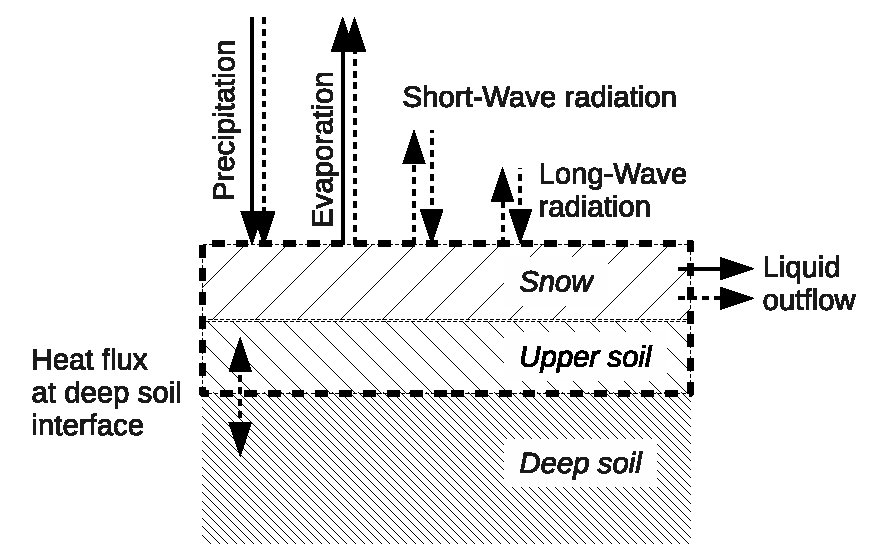
\includegraphics[width=0.48\textwidth]{\figdir/snow-fluxes.eps}
  \caption[Fluxes of mass and heat to be considered when simulating the snow dynamics.]{Fluxes of mass (solid arrows) and heat (dashed arrows) to be considered when simulating the snow dynamics. \label{fig:snow-enBal_snow-fluxes}}
\end{figure}

\begin{table*}
  \caption[Process matrix of the energy balance snow model.]{Process matrix of the energy balance snow model describing the dynamics of the state variables. The rate expressions containing state variables, forcings, and parameters are derived in \secref{sec:snow-enBal_fluxrates-energy} \& \ref{sec:snow-enBal_fluxrates-mass}. The stoichiometry factors \stoifacPrecMassToEnergy, \stoifacSublMassToEnergy, and \stoifacFlowMassToEnergy{} (kJ/\cbm) used to convert between mass and energy are derived in \secref{sec:snow-enBal_mass-energy-relations}. The $(+)$ indicates that precipitation has an impact on the albedo but this is considered a separate process called 'Albedo evolution' (see \secref{sec:snow-enBal_albedo}). \label{tab:snow-enBal_processmatrix}}
\begin{tabularx}{\textwidth}{|X|ccc|rr|} \hline
\rowcolor[gray]{0.9}
                  &  \multicolumn{3}{>{\columncolor[gray]{0.9}}c}{\textbf{Stoichiometry factors}}      &      &         \\
\rowcolor[gray]{0.9}
\textbf{Process}  & \snowEnergyContent & \snowWaterEquivalent & \snowAlbedo & \textbf{Rate expr.} & \textbf{Rate units} \\
\rowcolor[gray]{0.9}
                  & (kJ/\sqm)          & (m)                  & (--)        &                     &                     \\ \hline

Short-wave radiation balance & $0.001$ & $0$ & $0$ & \netRadiationShort & W/\sqm \\
Long-wave radiation balance  & $0.001$ & $0$ & $0$ & \netRadiationLong & W/\sqm \\
Soil heat flux               & $0.001$ & $0$ & $0$ & \heatfluxSoil & W/\sqm \\
Sensible heat flux           & $0.001$ & $0$ & $0$ & \heatfluxSens & W/\sqm \\
Precipitation                & $\stoifacPrecMassToEnergy$ & $1$ & $(+)$ & \massfluxPrec & m/s \\
Sublimation                  & $-\stoifacSublMassToEnergy$& $-1$ & $0$ & \massfluxSubl & m/s \\
Melt water outflow           & $-\stoifacFlowMassToEnergy$ & $-1$ & $0$ & \massfluxFlow & m/s \\
Albedo evolution             & $0$     & $0$ & $1$ & \albedoChangeRate & 1/s \\ \hline
\end{tabularx}
\end{table*}

\subsubsection{Definition of the energy content} \label{sec:snow-enBal_energy-content}
The energy content of the snow cover, \snowEnergyContent, can only be defined with respect to some reference. A useful reference state is ice at a temperature of 0\celsius{} for which \snowEnergyContent{} is zero by convention \citep{Tarboton1996}. With that reference, the relation between the energy content \snowEnergyContent{} and the (average) snow temperature \snowTemperature{} follows from the considerations below:

\begin{enumerate}

  \item Negative values of \snowEnergyContent{} indicate that \snowWaterEquivalent{} consists of solid water only and the snow temperature is negative. The relation between temperature and energy content is then determined by the heat capacity of the ice mass according to \eqnref{eqn:snow-enBal_heating-of-ice} (see \tabref{tab:snow-enBal_constants} for definition of symbols).
  \begin{equation} \label{eqn:snow-enBal_heating-of-ice}
    \frac{d\snowTemperature}{d\snowEnergyContent} = \frac{1}{\snowWaterEquivalent \cdot \densityWater \cdot \specHeatIce}
  \end{equation}

  With respect to the energy content, it is useful to treat the snow cover and the upper soil up to a certain depth \soilInteractionDepth{} as a single system (dashed box in \figref{fig:snow-enBal_snow-fluxes}). The upper soil is defined as the layer which thermally interacts with the snow cover on short time scales. Then, \eqnref{eqn:snow-enBal_heating-of-ice} expands to \eqnref{eqn:snow-enBal_heating-of-ice-soil-system}, where \soilInteractionDepth{} (m) represents the depth of the upper soil, \densitySoil{} (kg/\cbm) is the soil density and \specHeatSoil{} (kJ/kg/K) is the soil's specific heat capacity.
  \begin{equation} \label{eqn:snow-enBal_heating-of-ice-soil-system}
    \frac{d\snowTemperature}{d\snowEnergyContent} = \frac{1}{\snowWaterEquivalent \cdot \densityWater \cdot \specHeatIce + \soilInteractionDepth \cdot \densitySoil \cdot \specHeatSoil}
  \end{equation}

  Then advantage of treating the snow cover and the upper soil as a single system is that the soil energy flux reduces to the long-term average flux at the interface between shallow and deep soil (see \figref{fig:snow-enBal_snow-fluxes}). This flux is much less variable and may be approxiamed by a constant.

  \item If \snowEnergyContent{} is zero, the temperature is 0\celsius{} and the snow cover still does not contain liquid water as a consequence of the chosen reference.

  \item At positive values of \snowEnergyContent{}, some fraction of \snowWaterEquivalent{} exists in liquid form. As long as ice and liquid water coexist, the snow temperature remains at 0\celsius{} and all energy input is consumed by the melting process. The energy required to completely melt a snow cover at a temperature of 0\celsius{} which consists of solid water only is determined by the ice's heat of fusion (see \tabref{tab:snow-enBal_constants}) and equals (\eqnref{eqn:snow-enBal_melting-of-ice}):
  \begin{equation} \label{eqn:snow-enBal_melting-of-ice}
    \snowWaterEquivalent \cdot \densityWater \cdot \fusionHeatIce
  \end{equation}

  \item There is a critical value of \snowEnergyContent{} where all ice was melted and only liquid water is left. The snow has ceased to exist. If more energy is input, the temperature of the liquid water rises above zero according to \eqnref{eqn:snow-enBal_heating-of-water} (see \tabref{tab:snow-enBal_constants} for definition of symbols).
  \begin{equation} \label{eqn:snow-enBal_heating-of-water}
    \frac{d\snowTemperature}{d\snowEnergyContent} = \frac{1}{\snowWaterEquivalent \cdot \densityWater \cdot \specHeatWater}
  \end{equation}
\end{enumerate}

Based on these considerations, the relation between \snowEnergyContent{} and \snowTemperature{} can be computed for a snow cover with a given \snowWaterEquivalent{} as illustrated in \figref{fig:snow-enBal_energy-temperature-relation}.

\begin{figure}[htb]
  \centering
  \includegraphics[width=0.48\textwidth]{\figdir/snow-energy-temperature.eps}
  \caption[Relation between energy content and temperature for a sample snow cover.]{Relation between energy content and temperature for a sample snow cover with \snowWaterEquivalent= 0.05~m (soil interaction not taken into account). The thin vertical dashed line marks the (theoretical) energy content when the snow cover consists of liquid water only, \ie{} when all ice was melted. \label{fig:snow-enBal_energy-temperature-relation}}
\end{figure}

With the basic relations given by \eqnref{eqn:snow-enBal_heating-of-ice}--\ref{eqn:snow-enBal_heating-of-water} we can infer from the energy content \snowEnergyContent{} two important variables: the temperature \snowTemperature{} of the snow pack and the dimensionless fraction of liquid water \snowFractionLiquid.

\begin{table}[htb]
  \caption[Snow-related physical constants.]{Snow-related physical constants \citep{Tarboton1996,Dyck1995}. \label{tab:snow-enBal_constants}}
  \begin{tabularx}{0.48\textwidth}{|p{0.07\textwidth}rrX|} \hline
     \rowcolor[gray]{0.9}
     \textbf{Symbol}   & \textbf{Value}  & \textbf{Unit}    & \textbf{Description} \\ \hline
     \densityIce       & $\approx$922  & kg/\cbm & Density of ice \\
     \specHeatIce      & 2.09  & kJ/kg/K & Specific heat of ice \\
     \fusionHeatIce    & 333.5 & kJ/kg   & Latent heat of ice fusion (melt heat) \\
     \sublimHeatIce    & 2837  & kJ/kg   & Latent heat of ice sublimation (=\fusionHeatIce+\evapHeatWaterZero) \\
     \densityWater     & 1000  & kg/\cbm & Density of water \\
     \specHeatWater    & 4.18  & kJ/kg/K & Specific heat of water\\
     \evapHeatWaterZero & 2503  & kJ/kg & Latent heat of water evaporation at 0\celsius \\ \hline
  \end{tabularx}
\end{table}

\subsubsection{Snow temperature}
As the snow temperature is not simulated explicitly, it needs to be inferred from the state variables. Since snow is a good isolator, the snow surface temperature, \snowSurfaceTemperature{}, is generally different from the depth-averaged snow temperature \snowTemperature{} \citep{Tarboton1996}.

\paragraph{Depth-averaged temperature} Since the snow pack is assumed to be homogeneous, only the depth-averaged value, \snowTemperature{}, is directly accessible through the state variables \snowEnergyContent{} and \snowWaterEquivalent. Three cases need to be distinguished (see \secref{sec:snow-enBal_energy-content} for definition of \soilInteractionDepth{}, \densitySoil{} and \specHeatSoil{}):

\medskip\emph{Case 1: } ($\snowEnergyContent < 0$)
\begin{equation} \label{eqn:snow-enBal_energy-temperature-relation-allSolid}
  \snowTemperature= \frac{\snowEnergyContent}{\snowWaterEquivalent \cdot \densityWater \cdot \specHeatIce + \soilInteractionDepth \cdot \densitySoil \cdot \specHeatSoil}
\end{equation}

\medskip\emph{Case 2: } ($0 < \snowEnergyContent < \snowWaterEquivalent \cdot \densityWater \cdot \fusionHeatIce$)
\begin{equation} \label{eqn:snow-enBal_energy-temperature-relation-solidAndLiquid}
  \snowTemperature= 0
\end{equation}

\medskip\emph{Case 3: } ($\snowEnergyContent > \snowWaterEquivalent \cdot \densityWater \cdot \fusionHeatIce$)
\begin{equation} \label{eqn:snow-enBal_energy-temperature-relation-allLiquid}
  \snowTemperature= \frac{\snowEnergyContent - \snowWaterEquivalent \cdot \densityWater \cdot \fusionHeatIce}{\snowWaterEquivalent \cdot \densityWater \cdot \specHeatWater + \soilInteractionDepth \cdot \densitySoil \cdot \specHeatSoil}
\end{equation}

The equation for the first case (\eqnref{eqn:snow-enBal_energy-temperature-relation-allSolid}) directly follows from \eqnref{eqn:snow-enBal_heating-of-ice-soil-system} by multiplying with a negative $\Delta$\snowEnergyContent. The resulting temperature \snowTemperature{} is negative.

The conditions when \eqnref{eqn:snow-enBal_energy-temperature-relation-solidAndLiquid} must be used (second case) follow from the definition of \snowEnergyContent{} and \eqnref{eqn:snow-enBal_melting-of-ice}.

The third case (\eqnref{eqn:snow-enBal_energy-temperature-relation-allLiquid}) is considered here only for completeness since in represents the case where all snow became liquid, and \snowTemperature{} actually represents a water temperature.

\paragraph{Surface temperature} To compute energy fluxes across the snow-atmosphere interface (outgoing long wave radiation, exchange of sensible heat, etc.), an estimate of the surface temperature \snowSurfaceTemperature{} is required.

For estimating \snowSurfaceTemperature{}, \citet{Tarboton1996} assume that the energy fluxes at the snow surface are in equilibrium. \snowSurfaceTemperature{}, which controls some of the flux rates, is determined iteratively as the surface temperature where all energy fluxes balance. They also introduce a tuning parameter (snow surface conductance).

To avoid iteration, the very simple approach presented in \eqnref{eqn:snow-enBal_surfaceTemperature} is used here to estimate \snowSurfaceTemperature{}. Therein, \airtemp{} (\celsius) is the air temperature and $\mu$ is a weighting parameter. If $\mu=0$, the surface temperature \snowSurfaceTemperature{} is taken to be equal to the depth-averaged temperature \snowTemperature{} and if $\mu=0.5$, the surface temperature is simply computed as the mean of \snowTemperature{} and \airtemp. \eqnref{eqn:snow-enBal_surfaceTemperature} accounts for the fact that \snowSurfaceTemperature{} cannot become greater than 0~\celsius.

\begin{equation} \label{eqn:snow-enBal_surfaceTemperature}
  \snowSurfaceTemperature=
  \begin{cases}
     0 & \text{if \snowTemperature = 0} \\
     min(0, (1-\mu) \cdot \snowTemperature + \mu \cdot \airtemp) & \text{if \snowTemperature < 0} \\
  \end{cases}
\end{equation}

\subsubsection{Fraction of liquid water} \label{sec:snow-enBal_fractionLiquid}
In a melting snow cover, solid and liquid water coexist. To estimate the actual rate of water outflow, the fraction of liquid water, \snowFractionLiquid{} (--), must be known. Since \snowFractionLiquid{} is not simulated explicitly, it needs to be inferred from state variables. Taking into account that \snowFractionLiquid=0 if \snowEnergyContent=0 by definition and that the energy required to completely melt all ice (\snowFractionLiquid=1) is given by \eqnref{eqn:snow-enBal_melting-of-ice}, the liquid fraction can be computed from the energy content \snowEnergyContent{} as (\eqnref{eqn:snow-enBal_energy-fraction-liquid})

\begin{equation} \label{eqn:snow-enBal_energy-fraction-liquid}
  \snowFractionLiquid = \frac{\snowEnergyContent}{\snowWaterEquivalent \cdot \densityWater \cdot \fusionHeatIce}
\end{equation}

for $0 \le \snowEnergyContent \le \snowWaterEquivalent \cdot \densityWater \cdot \fusionHeatIce$, \ie{} for snow at 0~\celsius. Thus, in practice one should use something like $min(1,max(0,\snowFractionLiquid))$ if the condition is not checked explicitly. Note that \snowFractionLiquid{} represents a \emph{mass fraction} \citep{Tarboton1996}, not a volume fraction. Thus, \snowFractionLiquid{} can also be written as in \eqnref{eqn:snow-enBal_energy-fraction-liquid-masses}, where $m_w$ and $m_i$ represent the masses of water and ice per \sqm{} respectively.

\begin{equation} \label{eqn:snow-enBal_energy-fraction-liquid-masses}
  \snowFractionLiquid = \frac{m_w}{m_w + m_i}
\end{equation}

\eqnref{eqn:snow-enBal_energy-fraction-liquid-masses} may be transformed into \eqnref{eqn:snow-enBal_energy-fraction-liquid} as follows:

Numerator: As we are dealing with melting snow, the water mass $m_w$ is at 0~\celsius. Due to the definition of the energy content (see \secref{sec:snow-enBal_energy-content}), the mass $m_w$ (kg/\sqm) can be substituted by $\snowEnergyContent/\fusionHeatIce$.  \snowEnergyContent{} (kJ/\sqm) represents the energy content associated with $m_w$ and \fusionHeatIce{} is the fusion heat of ice (kJ/kg).

Denominator: The sum $m_w + m_i$ in the denominator of \eqnref{eqn:snow-enBal_energy-fraction-liquid-masses} represents the snow mass per square meter, $m_s$ (kg/\sqm). If $m_s$ is written as the product of snow density \densitySnow{} (kg/\cbm) and snow height \snowHeight{} (= snow volume per \sqm{} in meters), it follows from \eqnref{eqn:snow-enBal_defSWE} that the denominator $m_w + m_i$ equals $\snowWaterEquivalent \cdot \densityWater$.

\subsubsection{Relations between mass and energy fluxes} \label{sec:snow-enBal_mass-energy-relations}
In this section, the conversion factors \stoifacPrecMassToEnergy, \stoifacSublMassToEnergy, and \stoifacFlowMassToEnergy{} (kJ/\cbm) appearing in \tabref{tab:snow-enBal_processmatrix} are derived. The values of the involved physical constants can be found in \tabref{tab:snow-enBal_constants}.

\paragraph{Precipitation}
The energy flux (kJ/\sqm/s) resulting from precipitation input is obtained by multiplying the mass flux (m/s) with \stoifacPrecMassToEnergy{} (kJ/\cbm). For liquid precipitation, \stoifacPrecMassToEnergy{} is given by \eqnref{eqn:stoifacPrecMassToEnergy-rain} and \eqnref{eqn:stoifacPrecMassToEnergy-snow} applies to solid precipitation (snowfall). Note that precipitation is a water equivalent, thus, the density of water (not the one of ice) must be used when converting from depth (m) to mass (such as kg/\sqm).

\medskip\emph{Case 1: } ($\airtemp > \airtempRainSnow$)
\begin{equation}
  \stoifacPrecMassToEnergy = \densityWater \cdot \specHeatWater \cdot max(\airtemp,0) + \densityWater \cdot \fusionHeatIce \label{eqn:stoifacPrecMassToEnergy-rain}
\end{equation}

\medskip\emph{Case 2: } ($\airtemp <= \airtempRainSnow$)
\begin{equation}
  \stoifacPrecMassToEnergy = \densityWater \cdot \specHeatIce \cdot min(\airtemp,0) \label{eqn:stoifacPrecMassToEnergy-snow}
\end{equation}

In \eqnref{eqn:stoifacPrecMassToEnergy-rain} and \ref{eqn:stoifacPrecMassToEnergy-snow}, \airtemp{} (\celsius) is the air temperature and \airtempRainSnow{} (\celsius) is the threshold temperature for rain/snow fall. An approach for mixed precipitation is presented in \citet{Tarboton1996}. The value of \stoifacPrecMassToEnergy{} computed with \eqnref{eqn:stoifacPrecMassToEnergy-rain} is always positive and it is always negative if \eqnref{eqn:stoifacPrecMassToEnergy-snow} is ised. Note that the second term in \eqnref{eqn:stoifacPrecMassToEnergy-rain} accounts for the fact that the water is liquid and therefore has a positive energy content even at 0\celsius{} (see definition of \snowEnergyContent{} in \secref{sec:snow-enBal_energy-content}).

\paragraph{Sublimation}
The energy flux due to sublimation (kJ/\sqm/s) is obtained by multiplying the corresponding mass flux (m/s) with \stoifacSublMassToEnergy{} (kJ/\cbm) defined in \eqnref{eqn:stoifacSublMassToEnergy}. The constant \sublimHeatIce{} integrates the latent heat of both melting and evaporation (see \tabref{tab:snow-enBal_constants}). As heat is lost from the snow pack, the energy flux has a negative sign in \tabref{tab:snow-enBal_processmatrix}.
\begin{equation} \label{eqn:stoifacSublMassToEnergy}
  \stoifacSublMassToEnergy = \densityWater \cdot \sublimHeatIce
\end{equation}

\paragraph{Meltwater outflow}
To obtain the energy flux (kJ/\sqm/s) corresponding to the outflow of water from the snow pack (m/s) one has to multiply the latter by \stoifacFlowMassToEnergy{} (kJ/\cbm) defined in \eqnref{eqn:stoifacFlowMassToEnergy}. The expression reflects that the energy of water at 0\celsius{} equals \fusionHeatIce{} as a consequence of the chosen reference for \snowEnergyContent{} (see \secref{sec:snow-enBal_energy-content}). As heat is lost from the snow pack, the energy flux has a negative sign in \tabref{tab:snow-enBal_processmatrix}.
\begin{equation} \label{eqn:stoifacFlowMassToEnergy}
  \stoifacFlowMassToEnergy= \densityWater \cdot \fusionHeatIce
\end{equation}

%%%%%%%%%%%%%%%%%%%%%%%%%%%%%%%%%%%%%%%%%%%%%%%%%%%%%%%%%%%%%%%%%%%%%%%%%%%%%%%%
%%%%%%%%%%%%%%%%%%%%%%%%%%%%%%%%%%%%%%%%%%%%%%%%%%%%%%%%%%%%%%%%%%%%%%%%%%%%%%%%

\subsection{Simulation of the snow albedo} \label{sec:snow-enBal_albedo}

There are many approaches to estimate the snow albedo \snowAlbedo{} (--) with different level of sophistication. In general, the albedo is an average value accounting for the reflection of both visible and near infrared solar radiation. After snowfall, \snowAlbedo{} generally decreases due to various processes such as metamorphosis and pollution of the snow surface. Here, a very simple aging approach cited by \citet{Dyck1995} was adopted. The original equation to describe the dependence of \snowAlbedo{} on the age of the snow surface \citep[Equation 10.40 in][]{Dyck1995} is a power function (\eqnref{eqn:snow-enBal_albedo-powfunc}) where \snowAlbedoMin{} is the minimum value that \snowAlbedo{} approaches after a long time without snowfall and \snowAlbedoRng{} is the difference between the maximum \snowAlbedo{} right after snowfall and \snowAlbedoMin{}. Furthermore, \deltat{} is the age of the snow surface and $k$ (1/time) is a rate constant to describe the intensity of the aging process.

For convenience, \eqnref{eqn:snow-enBal_albedo-powfunc} was rewritten in an exponential form (\eqnref{eqn:snow-enBal_albedo-expfunc}) and \snowAlbedoRng{} was expanded to ($\snowAlbedoMax{}-\snowAlbedoMin{}$). In the final rearrangement, the new parameter \snowAlbedoDecrConst{} was introduced which is related to the parameter $k$ of the original power equation (\eqnref{eqn:snow-enBal_albedo-powfunc}) by $\snowAlbedoDecrConst = -k \cdot ln(\snowAlbedoMax-\snowAlbedoMin)$. Note that reasonable values of \snowAlbedo{} are $<1$ why $ln(\snowAlbedoMax-\snowAlbedoMin)$ is always negative and the minus sign is required to define \snowAlbedoDecrConst{} as a positive constant.

\begin{align}
  \snowAlbedo & = \snowAlbedoMin + {\snowAlbedoRng} ^{(1+\deltat \cdot k)} \label{eqn:snow-enBal_albedo-powfunc} \\
    & = \snowAlbedoMin + \snowAlbedoRng \cdot {\snowAlbedoRng} ^{\deltat \cdot k} \nonumber \\
    & = \snowAlbedoMin + \snowAlbedoRng \cdot exp(ln({\snowAlbedoRng} ^{\deltat \cdot k})) \nonumber \\
    & = \snowAlbedoMin + \snowAlbedoRng \cdot exp(\deltat \cdot k \cdot ln(\snowAlbedoRng)) \nonumber \\
    & = \snowAlbedoMin + (\snowAlbedoMax-\snowAlbedoMin) \cdot e^{-\snowAlbedoDecrConst \cdot \deltat} \label{eqn:snow-enBal_albedo-expfunc}
\end{align}

The advantage of \eqnref{eqn:snow-enBal_albedo-expfunc} over the original power function (\eqnref{eqn:snow-enBal_albedo-powfunc}) is the much simpler derivative with respect to time which is given in \eqnref{eqn:snow-enBal_albedo-expfunc-deriv}. Note that the definition of \snowAlbedo{} (\eqnref{eqn:snow-enBal_albedo-expfunc}) was used to simplify the derivative and that, in this way, the surfage age (\deltat) was eliminated from the expression.

\begin{align} \label{eqn:snow-enBal_albedo-expfunc-deriv}
  \frac{d \snowAlbedo}{dt} = & (\snowAlbedoMax - \snowAlbedoMin) \cdot e^{-\snowAlbedoDecrConst \cdot \deltat} \cdot (-\snowAlbedoDecrConst) \nonumber \\
                           = & (\snowAlbedo - \snowAlbedoMin) \cdot (-\snowAlbedoDecrConst)
\end{align}

Considering that the snow surface is renewed when new snow falls, the process rate \albedoChangeRate{} (1/s) controlling the albedo (see \tabref{tab:snow-enBal_processmatrix}) may be expressed by \eqnref{eqn:snow-enBal_albedo-agingRate}.

\begin{align} \label{eqn:snow-enBal_albedo-agingRate}
  \albedoChangeRate=
  \begin{cases}
     (\snowAlbedoMax - \snowAlbedo) & \text{if snowing} \\
     \snowAlbedoDecrConst(\airtemp) \cdot (\snowAlbedoMin - \snowAlbedo) & \text{else} \\
  \end{cases}
\end{align}

where $X=1$ if ((\precipIntensity > 0) \& (\airtemp < \airtempRainSnow)) and $X=0$ otherwise. Note that the applied value of the rate constant \snowAlbedoDecrConst{} depends on wether the air temperature is above or below 0~\celsius{} \citep{Dyck1995} . Thus, \albedoChangeRate{} is affected by both the precipitation intensity \precipIntensity{} and air temperature \airtemp. In the current model version, the albedo is independend of the snow height, \ie{} there is no reduction when the snow cover becomes shallow.

Recommended values of the parameters are given in \tabref{tab:snow-enBal_params-albedo}. A synthetic example illustrating the dynamics of the albedo in response to precipitation and temperature is shown in \figref{fig:snow-enBal_albedo-simExample}.

\begin{table}[htb]
  \caption[Parameters controlling the snow albedo.]{Parameters controlling the snow albedo based on \citet{Dyck1995}. With respect to \snowAlbedoDecrConst{}, the factor 1/86400 converts from 1/d to 1/s and the term $ln(\snowAlbedoMax-\snowAlbedoMin)$ accounts for the structural difference between \eqnref{eqn:snow-enBal_albedo-expfunc} and \eqnref{eqn:snow-enBal_albedo-powfunc}. \label{tab:snow-enBal_params-albedo}}
  \begin{tabularx}{0.48\textwidth}{|lrX|} \hline
  \rowcolor[gray]{0.9}
  Symbol & Units & Value \\ \hline
  \snowAlbedoMin  & -- & 0.35--0.4 \\
  \snowAlbedoMax  & -- & 0.75--0.9 \\
  \snowAlbedoDecrConst ($\airtemp \ge 0$) & 1/s & $-0.12/86400 \cdot ln(\snowAlbedoMax-\snowAlbedoMin)$ \\
  \snowAlbedoDecrConst ($\airtemp < 0$) & 1/s & $-0.05/86400 \cdot ln(\snowAlbedoMax-\snowAlbedoMin)$ \\
  \end{tabularx}
\end{table}

\begin{figure}[htb]
  \centering
  \includegraphics[width=0.35\textwidth]{\figdir/snow-albedo-simExample.eps}
  \caption[Synthetic example illustrating the dynamics of the albedo as affected by temperature and precipitation.]{Synthetic example illustrating the dynamics of the albedo as affected by temperature and precipitation. Snowfall was assumed at temperatures below 0~\celsius. For \snowAlbedoMin{} and \snowAlbedoMax{}, the means of the ranges given in \tabref{tab:snow-enBal_params-albedo} were used. \label{fig:snow-enBal_albedo-simExample}}
\end{figure}


%%%%%%%%%%%%%%%%%%%%%%%%%%%%%%%%%%%%%%%%%%%%%%%%%%%%%%%%%%%%%%%%%%%%%%%%%%%%%%%%
%%%%%%%%%%%%%%%%%%%%%%%%%%%%%%%%%%%%%%%%%%%%%%%%%%%%%%%%%%%%%%%%%%%%%%%%%%%%%%%%

\subsection{Energy flux rates} \label{sec:snow-enBal_fluxrates-energy}

\subsubsection{Short-wave radiation balance} \label{sec:snow-enBal_fluxrates-energy-shortwave}
The short-wave net radiation (or short-wave radiation balance), \netRadiationShort{} (W/\sqm) is computed from \eqnref{eqn:snow-enBal_netRadiationShort}

\begin{equation} \label{eqn:snow-enBal_netRadiationShort}
  \netRadiationShort = \solarRadiation \cdot (1-\snowAlbedo)
\end{equation}

where \solarRadiation{} is the incoming solar (\ie{} short-wave) radiation (W/\sqm) and \snowAlbedo{} (--) is the corresponding albedo of the snow surface (see \secref{sec:snow-enBal_albedo}). If measured values of \solarRadiation{} are unavailable, they can be estimated as described in \citet{Tarboton1996} or \citet{Dyck1995}. No corrections for slope and aspect are made here as it is assumed that the effects level out for larger areas. If the model is applied locally, slope and aspect might need to be taken into account by reducing/amplifying the measured (or computed) solar radiation for a horizontal surface.

The presence of a dense vegetation cover (coniferous forest) may considerably reduce the amount of incoming short-wave radiation. An ad-hoc approach to estimate the corrected incoming short-wave radiation \solarRadiation' due to shadowing is presented in \eqnref{eqn:snow-enBal_shadowing}

\begin{equation} \label{eqn:snow-enBal_shadowing}
  \solarRadiation' = \solarRadiation \cdot (1-\frac{\leafAreaIndex}{\leafAreaIndexFullShadow})
\end{equation}

where \leafAreaIndex{} is the leaf-area index (\sqm/\sqm) and \leafAreaIndexFullShadow{} is an empirical parameter. Conceptually, \leafAreaIndexFullShadow{} represents the leaf-area index where short-wave radiation is extincted completely. According to \citet{Ludwig2006}, a reduction of incoming short-wave by 30\% can be assumed for coniferous forest. Assuming a leaf-area index for coniferous forest of 11 \citep[][page 11]{Ludwig2006}, this results in $\leafAreaIndexFullShadow \approx 36$.


\subsubsection{Long-wave radiation balance}

The long-wave radation balance \netRadiationLong{} (W/\sqm) is the difference between the incoming long-wave radiation emitted from clear sky and clouds, \radLongwaveIn, and the long-wave emission of the snow pack, \radLongwaveOut{} (\eqnref{eqb:radBalanceLongwave}).

\begin{equation} \label{eqb:radBalanceLongwave}
  \netRadiationLong= \radLongwaveIn - \radLongwaveOut
\end{equation}

According to the Stefan-Boltzmann equation (\eqnref{eqn:stefan-boltzmann}), emissions $R$ are proportional to the fourth power of temperature \temperature{} (here in \celsius), with \stefanBoltzmann{} being the Stefan-Boltzmann constant (=5.67e-08 W/\sqm/K$^4$) and \emissivity{} being the dimensionless emissivity (range 0--1 with 1 for a black body).

\begin{equation} \label{eqn:stefan-boltzmann}
  R= \emissivity \cdot \stefanBoltzmann \cdot (T+273.15)^4
\end{equation}

\paragraph{Outgoing part}
The emission of the snow pack, \radLongwaveOut{} (W/\sqm), can directly be computed from \eqnref{eqn:stefan-boltzmann} substituting \temperature{} by the snow surface temperature \snowSurfaceTemperature{} (see \eqnref{eqn:snow-enBal_surfaceTemperature}). The emissivity of snow is about \emissivity=0.82 for old snow and \emissivity=0.99 for fresh snow \citep{Dyck1995}. A pragmatic way to account for the age of the snow pack is to relate \emissivity{} to the dynamically computed albedo \snowAlbedo{} (see \secref{sec:snow-enBal_albedo}) as in \eqnref{eqn:emissivity-estimation}.

\begin{equation} \label{eqn:emissivity-estimation}
  \emissivity = \emissivity_{min} + (\emissivity_{max} - \emissivity_{min}) \cdot \frac{\snowAlbedo - \snowAlbedoMin}{\snowAlbedoMax - \snowAlbedoMin}
\end{equation}

\paragraph{Incoming part}
Note: The following section is based on the German wikipedia site for the term 'Atmosphärische Gegenstrahlung' as this was the most transparent and concise source of information.

The incoming long-wave \radLongwaveIn{} is harder to estimate. Generally, it is distinguished between clear-sky emissions (\radLongwaveInClearsky{}) and emissions by clouds (\radLongwaveInClouds{}). A transparent formulation is given by \eqnref{eqn:radLongwaveIn} where \radLongwaveInClearsky{} and \radLongwaveInClouds{} are estimated individually and \cloudFraction{} represents the degree of cloud cover (range 0--1). It is (legitimately) assumed that long-wave emissions mainly stem from the lower atmoshpere (whose state is approximately known from ground measurements). 

\begin{equation} \label{eqn:radLongwaveIn}
  \radLongwaveIn = (1-\cloudFraction) \cdot \radLongwaveInClearsky + \cloudFraction \cdot \radLongwaveInClouds
\end{equation}

For the cloud cover \cloudFraction{} (--), measured values must be used or \cloudFraction{} needs to be estimated from a comparison of actual solar radiation to the theoretical maximum value depending on the day of the year and the latitude. However, the latter approach can only yield daily estimates of \cloudFraction{} as it does not work during nighttime.

\paragraph{Incoming part (Clear sky emissions)}
The clear sky radiation \radLongwaveInClearsky{} appearing in \eqnref{eqn:radLongwaveIn} is computed from the Stefan-Bolzmann equation (\eqnref{eqn:stefan-boltzmann}) substituting \temperature{} by the air temperature \airtemp{} and using a value of the emissivity \emissivity{} representative for a clear sky. \citet{Hock2005} lists various empirical formulas for estimation of the clear-sky \emissivity{} based on athmospheric temperature and/or vapor pressure. Some formulas are compared in \figref{fig:clearskyEmissivity}.

\begin{figure}[htb]
  \centering
  \includegraphics[width=0.35\textwidth]{\figdir/clearskyEmissivity.eps}
  \caption[Comparison of different empirical formulas for clear sky emissivity.]{Comparison of different empirical formulas for clear sky emissivity. \label{fig:clearskyEmissivity}}
\end{figure}

Here, we selected the simple formula developed by Brunt (\eqnref{eqn:emissivity-brunt}) which estimates the clear-sky \emissivity{} as a function of the vapor pressure \vaporPressure{} in hPa \citep[see][p.373]{Hock2005}.

\begin{equation} \label{eqn:emissivity-brunt}
  \emissivity = 0.51 + 0.066 \cdot \sqrt{\vaporPressure}
\end{equation}

\paragraph{Incoming part (Cloud emissions)}
Finally, the long-wave emissions of the clouds (\radLongwaveInClouds{} in \eqnref{eqn:radLongwaveIn}) are also computed using \eqnref{eqn:stefan-boltzmann}. The clouds are treated as a black body, thus \emissivity{} is set to 1. A reasonable estimate of the clouds' bottom-side temperature is the dew point temperature \dewpointTemperature{} (\celsius). \dewpointTemperature{} represents the temperature to which a parcel of air with a specific content of vapor must be cooled, for water vapor to condense. Thus, \dewpointTemperature{} is the temperature at which air with a specific vapor content becomes saturated. \dewpointTemperature{} can be computed by rearranging the Magnus-Equation (\eqnref{eqn:Magnus}) for the temperature \temperature{} (\eqnref{eqn:dewpointTemperature}). The reagrranged \eqnref{eqn:Magnus} yields the temperature at which, for a given vapor pressure, saturation would occur. Thus, the actual vapor pressure \vaporPressure{} (not \satVaporPressure{}) must be inserted in the rearranged \eqnref{eqn:Magnus}. If, as usual, only relative humidity and temperature are given, the value of \vaporPressure{} must be obtained from \eqnref{eqn:vaporPressure} with \satVaporPressure{} beign computed with \eqnref{eqn:Magnus} (now without rearrangement).

Thus, the dewpoint temperature \dewpointTemperature{} follows from \eqnref{eqn:dewpointTemperature} with \vaporPressure{} being computed from \relHumidity{} (\%) and \airtemp{} (\celsius) after \eqnref{eqn:Magnus}. Results for a range of temperatures and relative humidities are presented in \figref{fig:dewpointTemperature}.

\begin{equation} \label{eqn:dewpointTemperature}
  \dewpointTemperature =
  \begin{cases}
  \cfrac{237.3 \cdot log_{10}(\vaporPressure/6.11)}{7.5 - log_{10}(\vaporPressure/6.11)} & \text{over water} \\
  \cfrac{265.5 \cdot log_{10}(\vaporPressure/6.11)}{9.5 - log_{10}(\vaporPressure/6.11)} & \text{over ice} \\
  \end{cases}
\end{equation}

\begin{figure}[htb]
  \centering
  \includegraphics[width=0.48\textwidth]{\figdir/dewpoint-temperature.eps}
  \caption[Dewpoint temperature as a function of temperature and relative humidity.]{Dewpoint temperature as a function of temperature and relative humidity as computed with \eqnref{eqn:dewpointTemperature}. \label{fig:dewpointTemperature}}
\end{figure}

\subsubsection{Soil heat flux}
The soil heat flux \heatfluxSoil{} (W/\sqm) is, in this model, the long-term average flux at the interface between upper and deep soil (recall \secref{sec:snow-enBal_energy-content}). \heatfluxSoil{} is taken as zero if not known \citep{Tarboton1996}.

\subsubsection{Sensible heat flux} \label{sec:snow-enBal_fluxrates-energy_sensibleHeat}
The flux of sensible heat, \heatfluxSens{} (W/\sqm), is assumed to be proportional to the gradient of temperature between atmosphere (\airtemp) and snow surface (\snowSurfaceTemperature, see \eqnref{eqn:snow-enBal_surfaceTemperature}) as expressed by \eqnref{eqn:snow-enBal_heatfluxSens}. In this equation, \turbTransCoeff{} is a turbulent transfer coefficient (m/s), and \densityAir{} (kg/\cbm) and \specHeatAir{} (kJ/kg/K) represent the density and the specific heat capacity of air, respectively. This expression is equivalent to Equation 34 in \citet{Tarboton1996} or Equation 10.43 in \citet{Dyck1995}.

\begin{equation} \label{eqn:snow-enBal_heatfluxSens}
  \heatfluxSens = \turbTransCoeff \cdot \densityAir \cdot \specHeatAir \cdot 10^3 \cdot (\airtemp- \snowSurfaceTemperature)
\end{equation}

The value of the air specific heat capacity is \specHeatAir= 1.005~kJ/kg/K \citep{Tarboton1996}. The density of air \densityAir{} (kg/\cbm) is estimated from \eqnref{eqn:densityAir} \citep[see Equation 4.9 in][]{Dyck1995} that represents the ideal gas law (\airPressure: air pressure in hPa, \airtemp: air temperature in \celsius, specific gas constant for dry air: 0.287 kJ/kg/K, base of the Celsius-scale: 273.15~K).

\begin{equation} \label{eqn:densityAir}
  \densityAir = \frac{\airPressure \cdot 0.1}{0.287 \cdot (273.15 + \airtemp)}
\end{equation}

The values of \specHeatAir{} and \densityAir{} relate to dry air. However, the error in pressure due to neglection of moisture is rather low. Even at saturation, the vapor pressure is in the order of 0.5--2.5~\% of the air pressure only for temperatures between 0--25~\celsius{} (see \figref{fig:Magnus}). The error in the estimate of the specific heat capacity is small as well. The value is about 1.005~kJ/kg/K for dry air \citep{Tarboton1996} and about 1.013~kJ/kg/K for moist air \citep[][page 188, Eqn. 11.15]{Dyck1995}

The turbulent transfer coefficient \turbTransCoeff{} (m/s) in \eqnref{eqn:snow-enBal_heatfluxSens} is a calibration parameter. Several approaches to estimate \turbTransCoeff{} do exist \citep[e.~g.][]{Dyck1995, Tarboton1996} making assumptions on the stability of the atmosphere and introducing other unknown parameters. Here, as in \citet{Knauf1980}, a simple approach is used that assumes a linear dependence of \turbTransCoeff{} on the wind speed \windspeed{} in m/s according to \eqnref{eqn:turbTransCoeff-wind}. The empirical coefficients $a_0$ and $a_1$ are dimensionless and must be determined by calibration.

\begin{equation} \label{eqn:turbTransCoeff-wind}
  \turbTransCoeff = a_0 + a_1 \cdot \windspeed
\end{equation}

%%%%%%%%%%%%%%%%%%%%%%%%%%%%%%%%%%%%%%%%%%%%%%%%%%%%%%%%%%%%%%%%%%%%%%%%%%%%%%%%
%%%%%%%%%%%%%%%%%%%%%%%%%%%%%%%%%%%%%%%%%%%%%%%%%%%%%%%%%%%%%%%%%%%%%%%%%%%%%%%%

\subsection{Mass flux rates} \label{sec:snow-enBal_fluxrates-mass}

%%%%%%%%%%%%%%%%%%%%%%%%%%%%%%%%%%%%%%%%%%%%%%%%%%%%%%%%%%%%%%%%%%%%%%%%%%%%%%%%

\subsubsection{Precipitation}
The mass flux due to precipitation, \massfluxPrec{} (m/s), is computed from the precipitation intensity in units of mm/\deltat{} by \eqnref{eqn:snow-enBal_massfluxPrec} where \deltat{} is the length of the time step in seconds (\eg{} \deltat=3600 for hourly precipitation data).

\begin{equation} \label{eqn:snow-enBal_massfluxPrec}
  \massfluxPrec = \frac{\precipIntensity}{10^3 \cdot \deltat}
\end{equation}

The corresponding energy fluxes are given by \eqnref{eqn:stoifacPrecMassToEnergy-rain} \& \ref{eqn:stoifacPrecMassToEnergy-snow}, respectively.

%%%%%%%%%%%%%%%%%%%%%%%%%%%%%%%%%%%%%%%%%%%%%%%%%%%%%%%%%%%%%%%%%%%%%%%%%%%%%%%%

\subsubsection{Sublimation}
The mass flux due to sublimation, \massfluxSubl{} (m/s) is proportional to gradient of vapor pressure between the air and the snow surface as expressed by \eqnref{eqn:snow-enBal_massfluxSubl}. In this expression, \turbTransCoeff{} is a turbulent transfer coefficient (m/s), \densityAir{} and \densityWater{} (kg/\cbm) represent the densities of air and water. The symbols \specHumidity{} and \specHumiditySurface{} denote the specific humidities (--) above and at the snow surface, respectively. This expression is equivalent to Equation 35 in \citet{Tarboton1996} or Equation 10.44 in \citet{Dyck1995} (with changed sign) after multiplication with the density of water \densityWater{} to obtain the mass flux in kg/\sqm/s.

\begin{equation} \label{eqn:snow-enBal_massfluxSubl}
  \massfluxSubl = \turbTransCoeff \cdot \frac{\densityAir}{\densityWater} \cdot (\specHumiditySurface - \specHumidity)
\end{equation}

Only positive values of \massfluxSubl{} are considered. The density of (dry) air \densityAir{} is estimated from \eqnref{eqn:densityAir} (\secref{sec:snow-enBal_fluxrates-energy_sensibleHeat}). The specific humidity (--) can be computed from vapor pressure \vaporPressure{} and air pressure \airPressure{} (both in hPa) according to \eqnref{eqn:specHumidity} \citep[see Equation 4.10 in][]{Dyck1995}.

\begin{equation} \label{eqn:specHumidity}
  \specHumidity = \frac{0.622 \cdot \vaporPressure}{\airPressure - 0.378 \cdot \vaporPressure}
\end{equation}

Note that a commonly used approximation of \eqnref{eqn:specHumidity} is $\specHumidity \approx 0.622 \cdot \vaporPressure / \airPressure$ \citep{Dyck1995}. This approximation is used, for example, by \citet{Tarboton1996} in the derivation of their Equation 42. Note that they also substitute the pressure \airPressure{} by the product of temperature, air density, and the dry air gas constant according to the ideal gas law.

The vapor pressure \vaporPressure{} (hPa) is derived from the relative humidity \relHumidity{} (\%) by \eqnref{eqn:vaporPressure} taking into account the vapor pressure at saturation \satVaporPressure{} which is a function of temperature \temperature.

\begin{equation} \label{eqn:vaporPressure}
  \vaporPressure = \frac{\relHumidity}{100} \cdot \satVaporPressure(\temperature)
\end{equation}

\satVaporPressure{} is commonly estimated with the Magnus equation (\eqnref{eqn:Magnus}, \figref{fig:Magnus}) given by \citet{Dyck1995}. The temperature \temperature{} is the air temperature in \celsius.

\begin{equation} \label{eqn:Magnus}
  \satVaporPressure(T) =
  \begin{cases}
    6.11 \cdot 10^{\frac{7.5 \cdot \temperature}{237.3 + \temperature}} & \text{over water} \\
    6.11 \cdot 10^{\frac{9.5 \cdot \temperature}{265.5 + \temperature}} & \text{over ice} \\
  \end{cases}
\end{equation}

\begin{figure}[htb]
  \centering
  \includegraphics[width=0.35\textwidth]{\figdir/magnus-formula.eps}
  \caption[Saturation vapor pressure over water and ice as a function of temperature.]{Saturation vapor pressure over water and ice as a function of temperature (Magnus formula, \eqnref{eqn:Magnus}). \label{fig:Magnus}}
\end{figure}

When computing the input values for \eqnref{eqn:snow-enBal_massfluxSubl}, the saturation vapor pressure over ice (\second{} form of \eqnref{eqn:Magnus}) must be used. When calculating the specific humidity of the atmosphere (\specHumidity), one uses measured values of the air temperature, relative humidity, and air pressure in \eqnref{eqn:specHumidity} \& \ref{eqn:vaporPressure}. When computing the specific humidity at the snow surface (\specHumiditySurface), it is commonly assumed that the air is saturated at the surface temperature \citep{Tarboton1996}. Thus, one has to use $\relHumidity=100$ and $\temperature=\snowSurfaceTemperature$ in \eqnref{eqn:vaporPressure} (see \eqnref{eqn:snow-enBal_surfaceTemperature} for the surface temperature \snowSurfaceTemperature).

For the turbulent transfer coefficient \turbTransCoeff{} (m/s), the same value is assumed as for the transfer coefficient of sensible heat (see \eqnref{eqn:turbTransCoeff-wind} in \secref{sec:snow-enBal_fluxrates-energy_sensibleHeat}).

%%%%%%%%%%%%%%%%%%%%%%%%%%%%%%%%%%%%%%%%%%%%%%%%%%%%%%%%%%%%%%%%%%%%%%%%%%%%%%%%

\subsubsection{Melt water outflow}
The mass flux due to meltwater outflow, \massfluxFlow{} (m/s) equals the snow pack's actual hydraulic conductivity \citep[][cited in \citet{Tarboton1996}]{Male1981}. The actual hydraulic conductivity depends on both the saturated hydraulic conductivity \snowSatHydrCond{} (m/s) and the availablability of liquid water expressed by the relative saturation \snowRelSaturation{} (--) according to \eqnref{eqn:snow-enBal_massfluxFlow} \citep[see][]{Illangasekare1990}.

\begin{equation} \label{eqn:snow-enBal_massfluxFlow}
  \massfluxFlow = \snowSatHydrCond \cdot \snowRelSaturation^3
\end{equation}

The dimensionless relative saturation \snowRelSaturation{} is defined as the relative saturation in excess of water retained by capillary forces \citep{Illangasekare1990,Tarboton1996} and can be computed as:

\begin{equation} \label{eqn:snow-enBal_relSat-text}
  \snowRelSaturation{} = \frac{\text{liquid vol.}-\text{capillary retention vol.}}{\text{pore vol.}-\text{capillary retention vol.}}
\end{equation}

\citet{Tarboton1996} relate the capillary retention volume to the water equivalent of the solid matrix given by $\snowWaterEquivalent \cdot (1-\snowFractionLiquid)$. Thus, the whole \eqnref{eqn:snow-enBal_relSat-text} needs to be divided by this expression. For the single terms we obtain:

\paragraph{Capillary retention volume}
\begin{align*}
  & = \frac{\text{capillary retention volume}}{\snowWaterEquivalent \cdot (1-\snowFractionLiquid)} \\
  & = \snowRelCapRetent = \text{const.}
\end{align*}

\citet{Tarboton1996} suggest a value of 0.05 for the newly introduced constant \snowRelCapRetent.

\paragraph{Liquid volume}
\begin{align*}
  & = \frac{\text{liquid water volume}}{\snowWaterEquivalent \cdot (1-\snowFractionLiquid)} \\
  & = \frac{\snowWaterEquivalent \cdot \snowFractionLiquid}{\snowWaterEquivalent  \cdot (1-\snowFractionLiquid)} \\
  & = \frac{\snowFractionLiquid}{1-\snowFractionLiquid}
\end{align*}

\paragraph{Pore volume}
\begin{align*}
 & = \frac{\text{pore volume}}{\snowWaterEquivalent \cdot (1-\snowFractionLiquid)} \\
 & = \frac{\text{snow volume} - \text{solid water volume}}{\snowEnergyContent \cdot (1-\snowFractionLiquid)} \\
 & = \frac{\left( \cfrac{\text{mass of snow}}{\densitySnow} \right) - \left( \cfrac{\text{mass of ice}}{\densityIce} \right)}{\snowEnergyContent \cdot (1-\snowFractionLiquid)} \\
 & = \frac{ \left( \cfrac{\snowWaterEquivalent \cdot \densityWater}{\densitySnow} \right) - \left( \cfrac{\snowEnergyContent \cdot (1-\snowFractionLiquid) \cdot \densityWater}{\densityIce} \right)}{\snowEnergyContent \cdot (1-\snowFractionLiquid)} \\
 & = \frac{1}{1-\snowFractionLiquid} \cdot \frac{\densityWater}{\densitySnow} - \frac{\densityWater}{\densityIce}
\end{align*}

Collecting together all terms, \eqnref{eqn:snow-enBal_relSat-text} becomes \eqnref{eqn:snow-enBal_relSat-symb}.

\begin{equation} \label{eqn:snow-enBal_relSat-symb}
  \snowRelSaturation{} = \frac{\left( \cfrac{\snowFractionLiquid}{1-\snowFractionLiquid} \right)-\snowRelCapRetent}{\left( \cfrac{1}{1-\snowFractionLiquid} \cdot \cfrac{\densityWater}{\densitySnow} \right) - \left( \cfrac{\densityWater}{\densityIce} \right) - \snowRelCapRetent}
\end{equation}

\eqnref{eqn:snow-enBal_relSat-symb} is identical to Equation 48 in \citet{Tarboton1996} except for the term $1/(1-\snowFractionLiquid)$ in the denominator. The reason is that, although not explicitly stated, \citet{Tarboton1996} define \densitySnow{} in their equation 48 to be the \emph{dry snow density}, \densitySnowDry{}, which, as opposed to the common snow density \densitySnow{}, relates only for the mass of solid water to the snow volume and thus neglects the mass of liquid water \citep[see Equation 7 in][]{Morris1990}.

Recalling \eqnref{eqn:snow-enBal_energy-fraction-liquid-masses} from \secref{sec:snow-enBal_fractionLiquid}, the equality between $(1-\snowFractionLiquid) \cdot \densitySnow$ and \densitySnowDry{} can be demonstrated

\begin{align*}
 \densitySnowDry & = \frac{m_i}{v_s} \\
                 & = \frac{m_i \cdot m_s}{v_s \cdot m_s} \\
                 & = \densitySnow \cdot \frac{m_i}{m_s} \\
                 & = \densitySnow \cdot \frac{m_s-m_w}{m_s} \\
                 & = \densitySnow \cdot \left( 1- \frac{m_w}{m_s} \right) \\
                 & = \densitySnow \cdot ( 1- \snowFractionLiquid)
\end{align*}

where $m_i$, $m_w$, and $m_s$ (kg) represent masses of ice (solid), water (liquid), and snow (mixture of solid and liquid), respectively, and $v_s$ (\cbm) is the corresponding snow volume. Using \densitySnowDry{}, \eqnref{eqn:snow-enBal_relSat-symb} may be rewritten as \eqnref{eqn:snow-enBal_relSat-symb-dryDens} which is identical to Equation 48 in \citet{Tarboton1996}. They suggest for \densitySnowDry{} a value of 450 kg/\cbm.

\begin{equation} \label{eqn:snow-enBal_relSat-symb-dryDens}
  \snowRelSaturation{} = \frac{\left( \cfrac{\snowFractionLiquid}{1-\snowFractionLiquid} \right)-\snowRelCapRetent}{\left( \cfrac{\densityWater}{\densitySnowDry} \right) - \left( \cfrac{\densityWater}{\densityIce} \right) - \snowRelCapRetent}
\end{equation}

All in all, the rate of melt water outflow \massfluxFlow{} is controlled by the three free parameters listed in \tabref{tab:snow-enBal_params-massfluxFlow}.

\begin{table}[htb]
  \caption[Parameters controlling the rate of meltwater outflow.]{Parameters controlling the rate of meltwater outflow. Approximate values in brackets after \citet{Tarboton1996}. \label{tab:snow-enBal_params-massfluxFlow}}
  \begin{tabularx}{0.48\textwidth}{|lrX|} \hline
  \rowcolor[gray]{0.9}
  Symbol & Units & Description \\ \hline
  \snowSatHydrCond  & m/s & Saturated hydraulic conductivity. To be calibrated. \\
  \snowRelCapRetent & -- & Capillary retention volume as a fraction of the solid water equivalent. [$\approx$ 0.05]. \\
  \densitySnowDry   & kg/\cbm & Snow dry density [$\approx$ 450]. \\ \hline
  \end{tabularx}
\end{table}

%%%%%%%%%%%%%%%%%%%%%%%%%%%%%%%%%%%%%%%%%%%%%%%%%%%%%%%%%%%%%%%%%%%%%%%%%%%%%%%%
%%%%%%%%%%%%%%%%%%%%%%%%%%%%%%%%%%%%%%%%%%%%%%%%%%%%%%%%%%%%%%%%%%%%%%%%%%%%%%%%

\subsection{Test application} \label{sec:snow-enBal_test}

The energy balance model has been tested on daily data from two mountains in Germany. The two sites are 'Kahler Asten' (Lat: 51.1814, Lon: 8.4897, Elevation: 839 m) and 'Fichtelberg' (Lat: 50.4294, Lon: 12.9553, Elevation: 1213 m). Note that coordinates are in decimal degrees.

The required meteorological data were supplied by the German Weather Service (DWD) free of charge via the 'WEBVERDIS' interface. The data are in daily resolution and some post-processing was necessary to identify gaps and to remove duplicate records. Based on the data from the two mentioned sites, a common parameter set has been identified (\tabref{tab:snow-enBal_test-paramValues}) by carrying out a sequence of Monte-Carlo simulations with successive narrowing of the sampling ranges.

\begin{table}
  \caption{Calibrated parameters of the energy balance snow model based on daily data from two sites in Germany (Fichtelberg and Kahler Asten). \label{tab:snow-enBal_test-paramValues}}
\begin{tabular}{|lrl|} \hline
  \rowcolor[gray]{0.9}
  Parameter & Value & Corresp. eqn.(s) \\ \hline
  \airtempRainSnow & 0.2 & \eqnref{eqn:stoifacPrecMassToEnergy-rain} \\
  $\mu$ & 0.35 & \eqnref{eqn:snow-enBal_surfaceTemperature}\\
  $a0$ & 0.002 & \eqnref{eqn:turbTransCoeff-wind} \\
  $a1$ & 0.0008 & \eqnref{eqn:turbTransCoeff-wind} \\
  \emissivity$_{min}$ & 0.84 & \eqnref{eqn:emissivity-estimation} \\
  \emissivity$_{max}$ & 0.99 & \eqnref{eqn:emissivity-estimation} \\
  \densitySnowDry & 450 & \eqnref{eqn:snow-enBal_relSat-symb-dryDens} \\
  \snowSatHydrCond & 4.0e-05 & \eqnref{eqn:snow-enBal_massfluxFlow} \\
  \snowRelCapRetent & 0.05 & \eqnref{eqn:snow-enBal_relSat-symb-dryDens} \\
  \snowAlbedoMin  & 0.55 & \eqnref{eqn:snow-enBal_albedo-expfunc} \\
  \snowAlbedoMax  & 0.88 & \eqnref{eqn:snow-enBal_albedo-expfunc} \\
  \snowAlbedoDecrConst ($\airtemp \ge 0$) & 1.11e-06 & \eqnref{eqn:snow-enBal_albedo-expfunc} \\
  \snowAlbedoDecrConst ($\airtemp < 0$) & 4.62e-07 & \eqnref{eqn:snow-enBal_albedo-expfunc} \\
  \soilInteractionDepth & 0.1 & \eqnref{eqn:snow-enBal_heating-of-ice-soil-system} \\
  \densitySoil & 1300 & \eqnref{eqn:snow-enBal_heating-of-ice-soil-system} \\
  \specHeatSoil & 2.18 & \eqnref{eqn:snow-enBal_heating-of-ice-soil-system} \\
  \hline
\end{tabular}
\end{table}

A comparison of the observed and simulated snow water equivalent for the two test sites is provided in \figsref{fig:snow-enBal_test-Fichtelberg} \& \figref{fig:snow-enBal_test-KahlerAsten}. Note that only a selection of the data was used for model calibration. In particular, the focus was put on the melting phase since this is of special interest for flood forecasting.

\begin{figure*}
  \includegraphics[width=0.7\textwidth]{\figdir/test_Fichtelberg.eps}
  \caption{Observed and simulated snow water equivalent at DWD station 'Fichtelberg'. \label{fig:snow-enBal_test-Fichtelberg}}
\end{figure*}

\begin{figure*}
  \includegraphics[width=0.7\textwidth]{\figdir/test_KahlerAsten.eps}
  \caption{Observed and simulated snow water equivalent at DWD station 'Kahler Asten'. \label{fig:snow-enBal_test-KahlerAsten}}
\end{figure*}


%%%%%%%%%%%%%%%%%%%%%%%%%%%%%%%%%%%%%%%%%%%%%%%%%%%%%%%%%%%%%%%%%%%%%%%%%%%%%%%%
%%%%%%%%%%%%%%%%%%%%%%%%%%%%%%%%%%%%%%%%%%%%%%%%%%%%%%%%%%%%%%%%%%%%%%%%%%%%%%%%
%%%%%%%%%%%%%%%%%%%%%%%%%%%%%%%%%%%%%%%%%%%%%%%%%%%%%%%%%%%%%%%%%%%%%%%%%%%%%%%%

\section{Degree-day method} \label{sec:snow-degDay}

This method is currently \emph{not} implemented in an any \software{echse}-based hydrological models.





\chapter{Runoff generation} \label{chap:runGen}
\renewcommand{\tabdir}{chapters/part_processes/runoffGeneration/tab}
\renewcommand{\figdir}{chapters/part_processes/runoffGeneration/fig}

\section{Introduction} \label{sec:runGen_intro}

To avoid confusion, it is important to distinguish between the terms \emph{runoff generation} and \emph{runoff concentration}. As \emph{runoff generation}, we understand the transformation of water input (rain, snow melt) into runoff \emph{at the local scale}, \ie{} at every single point of a catchment. In contrast to that, the term \emph{runoff concentration} describes the transport of the locally generated runoff to the catchment's outlet (or the nearest river).

In some cases, the strict separation of the two terms is really pragmatic. However, it provides a clear and quite useful concept for hydrological catchment modeling.

%%%%%%%%%%%%%%%%%%%%%%%%%%%%%%%%%%%%%%%%%%%%%%%%%%%%%%%%%%%%%%%%%%%%%%%%%%%%%%%%
%%%%%%%%%%%%%%%%%%%%%%%%%%%%%%%%%%%%%%%%%%%%%%%%%%%%%%%%%%%%%%%%%%%%%%%%%%%%%%%%
%%%%%%%%%%%%%%%%%%%%%%%%%%%%%%%%%%%%%%%%%%%%%%%%%%%%%%%%%%%%%%%%%%%%%%%%%%%%%%%%

\section{Simple four components model} \label{sec:runGen4comp}

%%%%%%%%%%%%%%%%%%%%%%%%%%%%%%%%%%%%%%%%%%%%%%%%%%%%%%%%%%%%%%%%%%%%%%%%%%%%%%%%

\subsection{Processes and equations} \label{sec:runGen4comp_processes}

The four components runoff generation model described here is based on the concepts used in the LARSIM\footnote{Model variant '4Q-KOMP mit A2'} model \citet{Ludwig2006}. Originally, most equations were first presented by \citet{Todini1996}.

The runoff generation model is built upon the water balance of a soil column (\figref{fig:runGen4comp_soilWater}) which can be expressed by \eqnref{eqn:runGen4comp_soilWaterBalance}

\begin{equation} \label{eqn:runGen4comp_soilWaterBalance}
  \frac{d\soilWaterContent}{dt} = \frac{\rateWaterSupply - \rateRunoffSurf - \rateRunoffPref - \rateRunoffInter - \rateRunoffBase - \rateEvapotransp}{\soilDepth}
\end{equation}

with

\begin{tabular}{llp{0.6\columnwidth}}
\soilWaterContent & (--) & Soil water content as \cbm/\cbm \\
\rateWaterSupply & (m/s) & Rate of water supply (see \eqnref{eqn:runGen4comp_waterSupply}) \\
\rateRunoffSurf & (m/s) & Rate of surface runoff \\
\rateRunoffPref & (m/s) & Rate of quick sub-surface runoff (preferential flow) \\
\rateRunoffInter & (m/s) & Rate of slow sub-surface runoff (interflow) \\
\rateRunoffBase & (m/s) & Rate of deep percolation (rate of ground water recharge) \\
\rateEvapotransp & (m/s) & Rate of evapo(transpi)ration \\
\soilDepth & (m) & Depth (thickness) of soil column. \\
\end{tabular}

\medskip
The relevant thickness of the soil column \soilDepth{} is equivalent to the rooted depth. Soil water at greater depths is assumed (1) to be unavailable for evapotranspiration and (2) not to contribute to lateral runoff processes.

\begin{figure}
  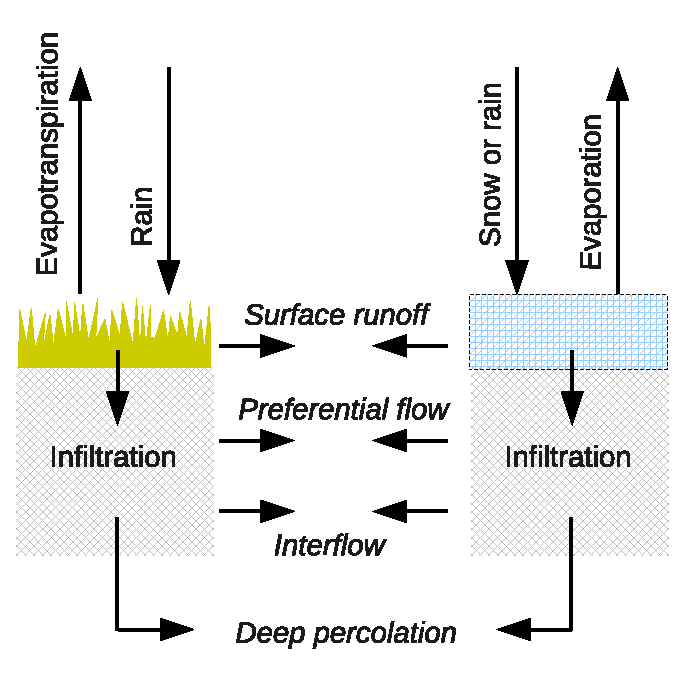
\includegraphics[width=0.9\columnwidth]{\figdir/soilWaterFluxes.eps}
  \caption{Water fluxes with respect to a soil column with (right) and without snow cover (left). \label{fig:runGen4comp_soilWater}}
\end{figure}

Snow coverage of the soil column is assumed to be either 0 or 100\%, \ie{} partial covering is \emph{not} simulated. As long as no snow is present, the rate of water supply to the soil column is the same as the intensity of precipitation, \precipIntensity{}. Once a snow cover exists, all precipitation is trapped in the snow and the rate of water supply is controlled by the melt rate, \rateSnowMelt{} (\eqnref{eqn:runGen4comp_waterSupply}). Both \precipIntensity{} and \rateSnowMelt{} are in units of m/s.

\begin{align} \label{eqn:runGen4comp_waterSupply}
  \rateWaterSupply =
  \begin{cases}
    \rateSnowMelt & \text{if snow cover is present} \\
    \precipIntensity & \text{else} \\
  \end{cases}
\end{align}

In the presented four components model, the generation of direct runoff\footnote{Runoff being quickly generated in response to water input.} is bound to the existence of (local) soil saturation. Thus, the model accounts for surface runoff due to infiltration excess but \emph{not} for Hortonian surface runoff.

Following to the Xinanjiang approach \citep{Zhao1980}, the fraction of saturated areas \satFrac{} in a catchment can be estimated from the area-integrated relative saturation of the soil \relSat{} which is the ratio of the current and maximum soil water content \soilWaterContent{} and \soilWaterContentMax{}, respectively (\eqnsref{eqn:runGen4comp_relativeSaturation} and \ref{eqn:runGen4comp_satFrac}). The rationale of the Xinanjiang model is a positive correlation between the catchment's average wetness, represented by the relative filling of the soil reservoir and the proportion of saturated areas. In other words, the occurrence of local saturation is assumed to increases as the catchment's average wetness becomes higher.

\begin{align}
  \relSat =& \frac{\soilWaterContent}{\soilWaterContentMax} \label{eqn:runGen4comp_relativeSaturation} \\
  \satFrac=& 1 - \left( 1 - \relSat \right) ^ \expSatFrac \label{eqn:runGen4comp_satFrac}
\end{align}

The shape of the relation between \relSat{} and \satFrac{} is controlled by a dimensionless empirical parameter \expSatFrac{}. The effect of different values of \expSatFrac{} is illustrated in \figref{fig:runGen4comp_expSatFrac}. A linear relation is assumed in the case $\expSatFrac{}=1$. Note that only values of $\expSatFrac{} \le 1$ are physically reasonable.
Max
\begin{figure}
  \includegraphics[width=0.9\columnwidth,angle=270]{\figdir/xinanjiang.eps}
  \caption[Influence of the empirical parameter \expSatFrac{}.]{Influence of the empirical parameter \expSatFrac{} on the relation between the catchment-integrated relative filling of the soil reservoir (x-axis) and the fraction of saturated areas \satFrac{} (y-axis). Only values of $\expSatFrac{} \le 1$ are physically reasonable. \label{fig:runGen4comp_expSatFrac}}
\end{figure}

The amount of direct runoff \heightRunoffDirect{} (in meters) is computed as a function of the fraction of saturated areas \satFrac{} according to \eqnref{eqn:runGen4comp_surfaceDirect}

\begin{align*}
  \heightRunoffDirect=
  \begin{cases}
    I - (W_m - W) + W_m \cdot x^{\expSatFrac+1}  & if (x > 0) \\
    I - (W_m - W)) & if (x \le 0)
  \end{cases}
\end{align*}

with

\begin{align} \label{eqn:runGen4comp_surfaceDirect}
  x=& \left(1-\frac{W}{W_m}\right)^{\left(\frac{1}{\expSatFrac+1}\right)} - \frac{I}{(1+\expSatFrac) \cdot W_m}
\end{align}

and $I$ being the total water input in a time step ($I= \rateWaterSupply \cdot \deltat$), $W$ being the amount of water in the modeled soil column ($W= \soilWaterContent \cdot \soilDepth$) and $W_m$ being the maximum capacity of the soil column ($W_m= \soilWaterContentMax \cdot \soilDepth$), all in units of meters. The derivation of this expression can be found in \citet{Todini1996} but is has to be noted that in this publication some signs are incorrect. The corrected version is presented in \citet{Bremicker2006}, for example. The relation between \heightRunoffDirect{} and $I$ according to \eqnref{eqn:runGen4comp_surfaceDirect} is illustrated in \figref{fig:runGen4comp_directRunoffHeight} for fix values of $W$ and $W_m$. A retention effect is visible for small to moderate water inputs. For water inputs considerably higher than the initial storage capacity of the soil, the relation between \heightRunoffDirect{} and $I$ becomes linear.

\begin{figure}
  \includegraphics[width=0.9\columnwidth,angle=270]{\figdir/arno.eps}
  \caption{Direct runoff computed with \eqnref{eqn:runGen4comp_surfaceDirect} for example values of soil storage and water input. \label{fig:runGen4comp_directRunoffHeight}}
\end{figure}

The model described here distinguished two components of direct runoff which differ with respect to retention characteristics. They may be considered as surface runoff and quick subsurface runoff through preferential flow paths. The proportion of the two components is controlled by a threshold value \thresholdSurf{} in units of m/s. The rates of surface runoff and quick subsurface runoff are computed according to \eqnref{eqn:runGen4comp_surfaceRunoff} and \eqnref{eqn:runGen4comp_prefRunoff}

\begin{align}
  \rateRunoffSurf =& max\left( 0, \frac{\heightRunoffDirect}{\deltat} - \thresholdSurf \right) \label{eqn:runGen4comp_surfaceRunoff} \\
  \rateRunoffPref =& \frac{\heightRunoffDirect}{\deltat} - \rateRunoffSurf \label{eqn:runGen4comp_prefRunoff}
\end{align}

Thus, if the rate of direct runoff production $\heightRunoffDirect/\deltat$ is below the threshold \thresholdSurf{}, only subsurface runoff is generated. Otherwise, surface runoff is generated from the excessive water. Note that the settings $\thresholdSurf{}=0$ or $\thresholdSurf{} \rightarrow \infty$ effectively result in a model with only 3 runoff components.

The generation of the slow runoff components is closely linked to the relative saturation of the soil \relSat{} (\eqnref{eqn:runGen4comp_relativeSaturation}). The rate of interflow runoff is computed by \eqnref{eqn:runGen4comp_interRunoff} using three empirical parameters. Here, \facInter{} represents a maximum rate of interflow runoff generation corresponding to total saturation of the soil. The actual rate, \rateRunoffInter{}, decreases at lower values of the soil saturation. If the saturation falls below a threshold level \relSatInter{}, no interflow runoff is generated at all. The shape of the soil moisture dependence is controlled by the empirical exponent \expInter{} whose effect is illustrated in \figref{fig:runGen4comp_powerExpression} (argument $s$ represents the fractional expression of \eqnref{eqn:runGen4comp_interRunoff}). The higher the value of the empirical exponent, the wetter the soil needs to be for interflow runoff becoming an important component. At very low values of \expInter{}, interflow runoff is produced almost at the maximum rate \facInter{}, as soon as the soil saturation exceeds the threshold \relSatInter{}. As in LARSIM, the parameter \expInter{} is treated as a constants with a value of 1.5 \citep{Bremicker2006}.

\begin{align} \label{eqn:runGen4comp_interRunoff}
  \rateRunoffInter =
  \begin{cases}
    \facInter \cdot \left( \frac{\relSat-\relSatInter}{1 - \relSatInter} \right) ^ \expInter & \text{if} \; \relSat > \relSatInter \\
    0 & \text{if} \; \relSat \le \relSatInter \\
  \end{cases}
\end{align}

\begin{figure}
  \includegraphics[width=0.9\columnwidth,angle=270]{\figdir/powerExpression.eps}
  \caption{Effect of the exponent $E$ in a formula $f=s^E$ for $s$ in range [0,1]. \label{fig:runGen4comp_powerExpression}}
\end{figure}

The rate of groundwater recharge (or base flow runoff), \rateRunoffBase{}, is computed by \eqnref{eqn:runGen4comp_baseRunoff} which is conceptually identical to \eqnref{eqn:runGen4comp_interRunoff}. Here, \facBase{} is the maximum rate of groundwater recharge which corresponds to a saturated soil. If the relative saturation of the soil falls below \relSatBase{}, the rate of groundwater recharge becomes zero. The shape of the dependence between \rateRunoffBase{} and \relSat{} is controlled by the empirical exponent \expBase{}. Again, the effect of this exponent can be seen from \figref{fig:runGen4comp_powerExpression} (argument $s$ represents the fractional expression of \eqnref{eqn:runGen4comp_baseRunoff}). As in LARSIM, the parameters \relSatBase{} and \expBase{} are treated as a constants with values of 0.05 and 1, respectively \citep{Bremicker2006}. Thus, only \facBase remains as a calibration parameter.

\begin{align} \label{eqn:runGen4comp_baseRunoff}
  \rateRunoffBase=
  \begin{cases}
    \facBase \cdot \left( \frac{\relSat-\relSatBase}{1 - \relSatBase} \right) ^ \expBase & \text{if} \; \relSat > \relSatBase \\
    0 & \text{if} \; \relSat \le \relSatBase \\
  \end{cases}
\end{align}

Of course, the theory described so far is only applicable to areas where soil water storage occurs. For areas covered by water or impervious surfaces, the rate of surface runoff \rateRunoffSurf{} equals the rate of rainfall or snow melt, respectively.

%%%%%%%%%%%%%%%%%%%%%%%%%%%%%%%%%%%%%%%%%%%%%%%%%%%%%%%%%%%%%%%%%%%%%%%%%%%%%%%%

\subsection{Combination with other models} \label{sec:runGen4comp_combination}
Depending on the model's purpose and local conditions, the described runoff generation model has to be augmented with
\begin{itemize}
  \item a model to compute snow storage and melt,
  \item a model to estimate evapotranspiration,
  \item an approach for precipitation correction (if not done externally).
\end{itemize}

%%%%%%%%%%%%%%%%%%%%%%%%%%%%%%%%%%%%%%%%%%%%%%%%%%%%%%%%%%%%%%%%%%%%%%%%%%%%%%%%

\subsection{Mathematical solution} \label{sec:runGen4comp_solution}

\eqnref{eqn:runGen4comp_soilWaterBalance} is an ordinary differential equation. Depending on the use of the model, a more of less sophisticated numerical solution has to be adopted. If computation times are critical (\eg{} in operational models), a simple \first{} order numerical solution may be preferable. Then, however, it needs special efforts to prevent unstable or unphysical solutions. In particular, in the absence of appropriate correction terms, a \first{} oder solution of \eqnref{eqn:runGen4comp_soilWaterBalance} may yield a computed soil moisture \soilWaterContent{} which is negative.

%%%%%%%%%%%%%%%%%%%%%%%%%%%%%%%%%%%%%%%%%%%%%%%%%%%%%%%%%%%%%%%%%%%%%%%%%%%%%%%%

\subsection{Implementation} \label{sec:runGen4comp_implementation}

\tabref{tab:runGen4comp_implementation} relates the identifier names used in the model implementation (names of state variables and parameters) to the symbols used in the process equations (\secref{sec:runGen4comp_processes}). Additional information that may be helpful when calibrating a model without any prior knowledge of parameter values is given in \secref{sec:runGen4comp_hints}.

\begin{table*}
\caption{Symbols used in the process equations (\secref{sec:runGen4comp_processes}), corresponding identifiers, and hints for calibration. \label{tab:runGen4comp_implementation}}
\begin{tabular}{|p{0.07\textwidth}p{0.15\textwidth}p{0.1\textwidth}p{0.15\textwidth}p{0.35\textwidth}|}  \hline
\rowcolor[gray]{0.9}
Symbol & Identifier & Units & Typical values & Details \\ \hline
\soilWaterContent & \verb!wc! & -- & -- & Computed state variable \\
\soilDepth & \verb!soildepth! & m & Rooted depth & -- \\
\soilWaterContentMax & \verb!wc_max! & -- & 0.4--0.5 & \tabref{tab:et:real:soilmoisture} on page \pageref{tab:et:real:soilmoisture} \\
\expSatFrac & \verb!exp_satfrac! & -- & 0.01--1 & See \figref{fig:runGen4comp_expSatFrac} \\
\thresholdSurf & \verb!thr_surf! & m/s & --  & Values of 0 or near $\infty$ result in a 3 components model (see \eqnsref{eqn:runGen4comp_surfaceRunoff} \& \ref{eqn:runGen4comp_prefRunoff} ). \\
\relSatInter & \verb!relsat_inter! & -- & 0.5 -- 0.8 & Number between 0 and 1. \\
\rateRunoffInter & \verb!rate_inter! & m/s & example: 1.e-07 & Depends on hydraulic conductivity \\
\rateRunoffBase & \verb!rate_base! & m/s & example: 1.e-08 & Depends on hydraulic conductivity \\
\end{tabular}
\end{table*}

\subsection{Hints for application} \label{sec:runGen4comp_hints}

The parameter \facBase{} specifies the rate of deep percolation under the conditions of a fully saturated soil (\eqnref{eqn:runGen4comp_baseRunoff}). At a first glance, it seems as if \facBase{} could be estimated from the soil's saturated hydraulic conductivity \satHydrCond{}. However, at high values of the soil moisture, the other runoff components are also active and, typically, these other components are much more effective in draining the soil. Consequenty, we can expect \facBase{} $\ll$ \satHydrCond{}.

A more promising approach to estimate \facBase{} relies on the analysis of a discharge hydrograph (\figref{fig:runGen4comp_parEstim_facBase}). In this figure, an approxiate hydrograph of the base flow component was added. It can be drawn by hand as a smooth line connecting the annual minimum values (low flows) also touching the minima during the rainy season. Obviously, the hydrograph of the base flow component has, like any periodic function, two types of turning points. For convenience, we focus on the lower turning points here. They are easier to identify from the data without the need for any drawing, actually.

\begin{figure}
  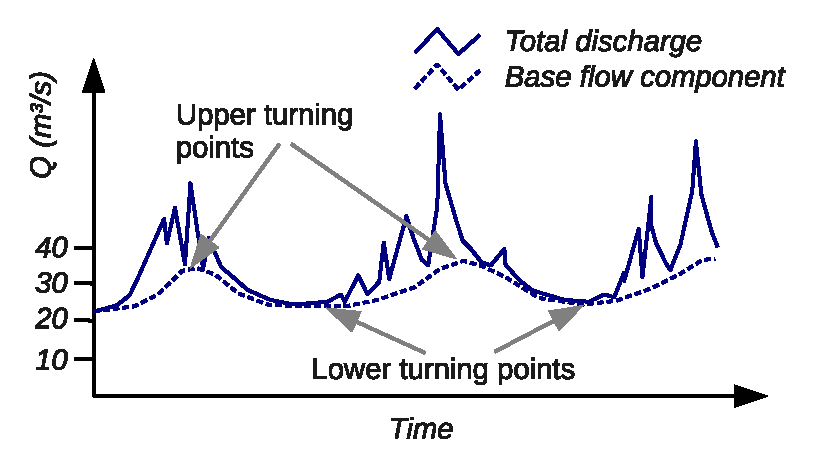
\includegraphics[width=0.9\columnwidth]{\figdir/parEstim_facBase.eps}
  \caption{Discharge hydrograph with manually separated base flow component. \label{fig:runGen4comp_parEstim_facBase}}
\end{figure}

In the following we assume that the base flow component is equivalent to the outflow from a conceptual ground water reservoir. For simplicity, we may consider a linear reservoir described by \eqnsref{eqn:runConcParStor_linResBalance} \& \ref{eqn:runConcParStor_linResOutflow} (see page \pageref{eqn:runConcParStor_linResBalance}). From the differential equation, we find that, at the mentioned turning points, the derivative of the storage volume with respect to time becomes zero, hence the rates of inflow and outflow are equal. Consequently, the \emph{base flow rate} at the turning points in a plot like \figref{fig:runGen4comp_parEstim_facBase} directly yields an estimate of the \emph{rate of ground water recharge}, \rateRunoffBase{}, at the respective point in time.

The relation between the actual rate of ground water reacharge \rateRunoffBase{} and the model parameter \facBase{} is given by \eqnref{eqn:runGen4comp_baseRunoff}. This can be rearranged and \rateRunoffBase{} can be substituted by $A \cdot Q_{base}$ where $A$ is the size of the catchment in units of \sqm{} and $Q_{base}$ is the base flow component in \cbms{} (\eqnref{eqn:runGen4comp_parEstim_facBase}). Using the fixed values of \relSatBase{} and \expBase{} mentioned in  \secref{sec:runGen4comp_processes}, we end up with \eqnref{eqn:runGen4comp_parEstim_facBase_final}.

\begin{eqnarray}
  \facBase &=& \dfrac{Q_{base}}{A} \cdot \left( \dfrac{\relSat-\relSatBase}{1 - \relSatBase} \right) ^ {-\expBase} \label{eqn:runGen4comp_parEstim_facBase} \\
           &=& \dfrac{Q_{base}}{A} \cdot \left( \dfrac{0.95}{\relSat - 0.05} \right) \label{eqn:runGen4comp_parEstim_facBase_final}
\end{eqnarray}

In order to calculate \facBase{} from \eqnref{eqn:runGen4comp_parEstim_facBase_final} we have to supply an estimate of the soil saturation \relSat{} at the respective point in time (\ie{} the analyzed turning point). For the lower turning points, a reasonable guess can be obtained from the soil water content at the wilting point. For a silty soil, for example, the saturation \relSat{} would be $\approx$ 0.2 for a soil moisture at the wilting point of 0.1 and a maximum water content of 0.48 (see \tabref{tab:et:real:soilmoisture} on page~\pageref{tab:et:real:soilmoisture}).

The value of \facBase{} obtained from the hydrograph analysis is a crude estimate. However, it might help in the definition of a proper search range for \facBase{} in the context of automatic model calibration.

\chapter{Runoff concentration} \label{chap:runConc}
\renewcommand{\tabdir}{chapters/part_processes/runoffConcentration/tab}
\renewcommand{\figdir}{chapters/part_processes/runoffConcentration/fig}

\section{Introduction} \label{sec:runConc_intro}

The term \emph{runoff concentration} describes the transport of the locally generated runoff (see \chapref{chap:runGen}) to the catchment's outlet or the nearest river. In general, the description of water transport covers the phenomena of translation and retention.


%%%%%%%%%%%%%%%%%%%%%%%%%%%%%%%%%%%%%%%%%%%%%%%%%%%%%%%%%%%%%%%%%%%%%%%%%%%%%%%%
%%%%%%%%%%%%%%%%%%%%%%%%%%%%%%%%%%%%%%%%%%%%%%%%%%%%%%%%%%%%%%%%%%%%%%%%%%%%%%%%
%%%%%%%%%%%%%%%%%%%%%%%%%%%%%%%%%%%%%%%%%%%%%%%%%%%%%%%%%%%%%%%%%%%%%%%%%%%%%%%%

\section{Parallel storage model} \label{sec:runConcParStor}

%%%%%%%%%%%%%%%%%%%%%%%%%%%%%%%%%%%%%%%%%%%%%%%%%%%%%%%%%%%%%%%%%%%%%%%%%%%%%%%%

\subsection{Processes and equations} \label{sec:runConcParStor_processes}

In the parallel storage model, it is assumed that runoff concentration can be computed separately for the individual runoff components. For each component, translation and retention is simulated by means of a simple reservoir model. The cumulated runoff from the parallel reservoirs finally represents the sub-basins total runoff (\figref{fig:runConcParStor_scheme}).

\begin{figure}
  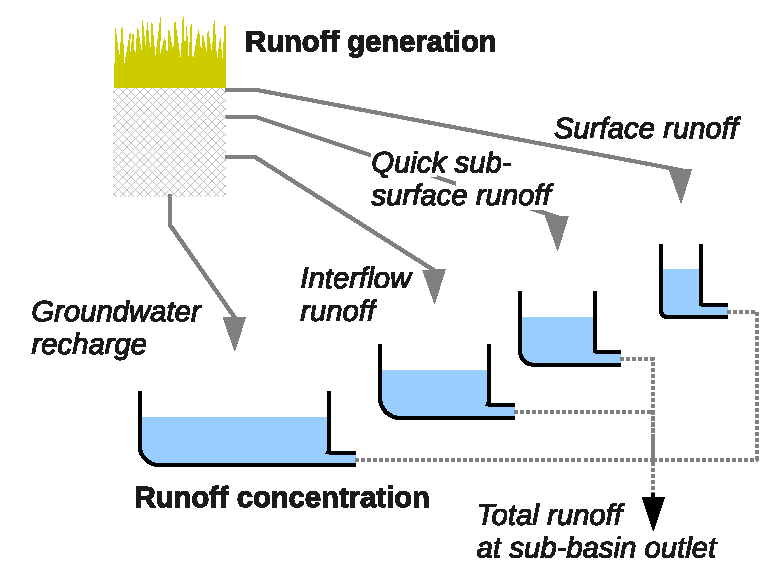
\includegraphics[width=0.9\columnwidth]{\figdir/parallelStorage.eps}
  \caption{Parallel storage model for the case of four runoff components. \label{fig:runConcParStor_scheme}}
\end{figure}

Following the approach used in LARSIM \citep{Ludwig2006}, all reservoirs depicted in \figref{fig:runConcParStor_scheme} are of the linear type. Thus, in addition to the mass balance (\eqnref{eqn:runConcParStor_linResBalance}), the linear relation of \eqnref{eqn:runConcParStor_linResOutflow} applies to each reservoir.

\begin{equation} \label{eqn:runConcParStor_linResBalance}
  \frac{dv}{dt} = q_{in} - q_{out}
\end{equation}
\medskip
\begin{tabular}{lll}
  $v$ & Storage volume & L$^3$ \\
  $q_{in}$ & Inflow rate & L$^3$/T\\
  $q_{out}$ & Outflow rate & L$^3$/T\\
\end{tabular}

\begin{equation} \label{eqn:runConcParStor_linResOutflow}
  q_{out}= \frac{1}{k} \cdot v
\end{equation}
\medskip
\begin{tabular}{lll}
  $k$ & Retention constant & T \\
\end{tabular}

\eqnsref{eqn:runConcParStor_linResBalance} and \ref{eqn:runConcParStor_linResOutflow} can be combined and integrated over time using the substitution method. Assuming that the inflow rate $q_{in}$ is constant over a discrete time step, the integration yields \eqnref{eqn:runConcParStor_linResSolution} as the solution for the storage volume.

\begin{equation} \label{eqn:runConcParStor_linResSolution}
  v(t_0 + \Delta t) =  (v(t_0) - q_{in} \cdot k) \cdot e^{(-\Delta t / k)} + q_{in} \cdot k
\end{equation}
\medskip
\begin{tabular}{lll}
  $v(t_0)$ & Initial storage at & L$^3$ \\
  $\Delta t$ & Length of time step & T \\
\end{tabular}

The only parameters in this runoff concentation model are the values of the retention constants $k$ (one for each reservoir shown in \figref{fig:runConcParStor_scheme}. Regarding these constants, we can formulate two expectations:

\begin{enumerate}
  \item Larger values of $k$ result in a higher retention effect and thus in a more delayed input-output reaction (\figref{fig:runConcParStor_singleLinReserv}). Consequently, we expect the highest $k$ value for the groundwater reservoir while the smallest $k$ value corresponds to the reservoir describing the concentration of surface runoff.
  \item Furthermore, it seems legitimate to assume a relation between the $k$ values and the characteristics of a sub-basin. In particular, we expect smaller retention constants in regions with steep hill slopes, dense drainage networks, and for sub-basin of compact shape.
\end{enumerate}

\begin{figure}
  \includegraphics[width=0.9\columnwidth,angle=270]{\figdir/singleLinearReservoir.eps}
  \caption{Outflow hydrographs from a single linear reservoir for an identical input signal but different storage constants $k$ (hours). \label{fig:runConcParStor_singleLinReserv}}
\end{figure}

To take these two aspect into account, it is convenient to define the retention constants as in \eqnsref{eqn:runConcParStor_retConstSurf} to \ref{eqn:runConcParStor_retConstBase}.

\begin{align}
\text{Surface runoff:} && k = \strSurf \cdot \concTimeIndex \label{eqn:runConcParStor_retConstSurf} \\
\text{Preferential flow:} && k = \strPref \cdot \concTimeIndex \label{eqn:runConcParStor_retConstPref} \\
\text{Interflow:} && k = \strInter \cdot \concTimeIndex \label{eqn:runConcParStor_retConstInter} \\
\text{Base flow:} && k = \strBase \cdot \concTimeIndex \label{eqn:runConcParStor_retConstBase}
\end{align}

Here, \strSurf, \strPref, \strInter, and \strBase{} are dimensionless calibration parameters, fulfilling $\strSurf < \strPref < \strInter < \strBase$ (recall \first{} point of above enumeration). Furthermore, \concTimeIndex{} is an indicator of the sub-basin's runoff concentration characteristics having the dimension of a time (\second{} point of above enumeration). For estimating the \concTimeIndex{} different approaches do exist. In LARSIM \citep{Ludwig2006}, for example, an empirical formula derived by \citet{Kirpich1940} is used. This one computes the \concTimeIndex{} from the average length and slope of the major reach(es) in a sub-basin. Alternatively, a \concTimeIndex{} can be derived by analysis of a digital elevation model. This approach is described in the documentation of the \software{topocatch} preprocessor \citep[see][]{Echse-Tools-Doc}.

See \secref{sec:runConcParStor_hints} for the relation between the $k$ values and the half-life time \halflife{}.

The inflow rate $q_{in}$ (\cbm/s) appearing in \eqnsref{eqn:runConcParStor_linResBalance} to \ref{eqn:runConcParStor_linResSolution} is generally obtained by multiplying the runoff rate (m/s) by the contributing area (\sqm). For the reservoir describing the concentration of surface runoff, $q_{in}$ is usually composed of the runoff generated on saturated soils, water surfaces, and also impervious surfaces.

%%%%%%%%%%%%%%%%%%%%%%%%%%%%%%%%%%%%%%%%%%%%%%%%%%%%%%%%%%%%%%%%%%%%%%%%%%%%%%%%

\subsection{Mathematical solution} \label{sec:runConcParStor_solution}

In each time step, the storage of the four reservoirs is updated based on \eqnref{eqn:runConcParStor_linResSolution} using the individual inflow rates and retention constants (\eqnsref{eqn:runConcParStor_retConstSurf} to \ref{eqn:runConcParStor_retConstBase}). The total outflow from a sub-basin is then obtained as the sum of the outflow rates from the four linear reservoirs.

Note that, if \eqnref{eqn:runConcParStor_linResOutflow} is applied to the already updated storage volumes, the computed outflow rates are \emph{instantaneous values} which correspond to the \emph{end} of a time step. To ensure conservation of mass, these rates should not be directly used as inputs for a downstream model (usually a flow routing model). Instead, \emph{time-step averaged} outflow rates must be passed to the downstream model. For each reservoir, the time-step averaged outflow rates are obtained from the discrete version of the mass balance equation (recall \eqnref{eqn:runConcParStor_linResBalance}) as shown in \eqnref{eqn:runConcParStor_averageOutflow}.

\begin{equation} \label{eqn:runConcParStor_averageOutflow}
  \overline{q_{out}} = q_{in} - \frac{v(t_0 + \Delta t) - v(t_0)}{\Delta t}
\end{equation}
\medskip
\begin{tabular}{lll}
  $\overline{q_{out}}$ & Time-step averaged outflow rate & L$^3$/T\\
  $q_{in}$ & Inflow rate (constant over $\Delta t$) & L$^3$/T \\
  $v(t_0)$ & Initial storage volume & L$^3$ \\
  $v(t_0 + \Delta t)$ & Storage at end of time step & L$^3$ \\
\end{tabular}

%%%%%%%%%%%%%%%%%%%%%%%%%%%%%%%%%%%%%%%%%%%%%%%%%%%%%%%%%%%%%%%%%%%%%%%%%%%%%%%%

\subsection{Implementation} \label{sec:runConcParStor_implementation}

\tabref{tab:runConcParStor_implementation} relates the identifier names used in the model implementation (names of state variables and parameters) to the symbols used in the process equations (\secref{sec:runConcParStor_processes}).

\begin{table*}
\caption{Symbols used in the process equations (\secref{sec:runConcParStor_processes}) and  corresponding identifiers. \label{tab:runConcParStor_implementation}}
\begin{tabular}{|p{0.2\textwidth}p{0.13\textwidth}p{0.07\textwidth}p{0.42\textwidth}|}  \hline
\rowcolor[gray]{0.9}
Symbol & Identifier & Units & Details \\ \hline
$v$ (surface runoff) & \verb!vol_surf! & \cbm{} & Storage volume of surface runoff reservoir \\
$v$ (preferential flow) & \verb!vol_pref! & \cbm{} & Storage volume of preferential flow reservoir \\
$v$ (interflow) & \verb!vol_inter! & \cbm{} & Storage volume of interflow reservoir \\
$v$ (baseflow) & \verb!vol_base! & \cbm{} & Storage volume of baseflow reservoir \\
\strSurf & \verb!str_surf! & sec & Retention constant of surface runoff reservoir \\
\strPref & \verb!str_pref! & sec & Retention constant of preferential flow reservoir \\
\strInter & \verb!str_inter! & sec & Retention constant of interflow reservoir \\
\strBase & \verb!str_base! & sec & Retention constant of baseflow reservoir \\ \hline
\end{tabular}
\end{table*}

%%%%%%%%%%%%%%%%%%%%%%%%%%%%%%%%%%%%%%%%%%%%%%%%%%%%%%%%%%%%%%%%%%%%%%%%%%%%%%%%

\subsection{Hints for application} \label{sec:runConcParStor_hints}

As with all state variables, initial values must be assigned to the storage volumes listed in \tabref{tab:runConcParStor_implementation}. These values are generally unknown and cannot be derived from observation data. Therefore, a widely used approach is to simply guess the initial values and to allow for a rather long 'warm-up' period of the model (several years). If boundary condition data are available for a limited period of time only, one should run a sequence of warm-up simulations. Guessed initial values are used only in the first run. In all later runs, the model is initialized with the final state of the previous run. The success of the latter strategy can be checked, for example, by plotting some simulated hydrographs. If the differences between the hydrographs of consecutive runs becomes negligible, the desired equilibrium of the storage volumes has been reached. However, even then, the initial part of a simulated time series should not be compared to observations because the initial state is still a (refined) guess.

The retention constants listed in \tabref{tab:runConcParStor_implementation} need to be identified by calibration. The values depend on the characteristics of the modeled basin, the model's resolution, as well as on the definition of the used concentraction time index, \concTimeIndex{} (see \eqnsref{eqn:runConcParStor_retConstSurf} to \ref{eqn:runConcParStor_retConstBase}). When calibrating the retention constants, one should keep in mind that a particular parameter set is reasonable only if $\strSurf < \strPref < \strInter < \strBase$ (see \secref{sec:runConcParStor_processes} for details).

The time for model calibration can be reduced (and the overall chance of success can be increased), if prior knowledge on the magnitude of the retention constants is available. If a calibrated model for another nearby basin is available, one could try to adopt the values used in this model as initial guesses. However, this will only work if the basins' characteristics in terms of climate, geomorphology, and land-use are really comparable. Furthermore, the two models must also be comparable with respect to the spatial and temporal discretization.

If another model for a nearby basin is not available or the mentioned conditions are not met, one can try to infer estimates of the retention constants from observed discharge hydrographs. For that purpose, one has to analyze the shape of stream flow recessions using the theory of the single linear reservoir.

Substituting the volume $v$ in \eqnref{eqn:runConcParStor_linResSolution} using \eqnref{eqn:runConcParStor_linResOutflow} yields an equation to predict the future outflow of a linear reservoir using a known initial outflow rate (\eqnref{eqn:runConcParStor_linResSolution_flow}).

\begin{equation} \label{eqn:runConcParStor_linResSolution_flow}
  q_{out}(t_0 + \Delta t) =  (q_{out}(t_0) - q_{in}) \cdot e^{(-\Delta t / k)} + q_{in}
\end{equation}

During recession some time after a flow peak, we can assume that the outflow from the reservoir is much higher than the inflow. Assuming zero inflow, \eqnref{eqn:runConcParStor_linResSolution_flow} simplifies to \eqnref{eqn:runConcParStor_linResSolution_flow_zeroInput}

\begin{equation} \label{eqn:runConcParStor_linResSolution_flow_zeroInput}
  q_{out}(t_0 + \Delta t) =  q_{out}(t_0) \cdot e^{(-\Delta t / k)}
\end{equation}

which can then be solved for the storage constant $k$ (\eqnref{eqn:runConcParStor_kEstim}). Note that all values appearing at the right hand side of this equation are easily obtained from a hydrograph plot (\figref{fig:runConcParStor_recession}).

\begin{equation} \label{eqn:runConcParStor_kEstim}
  k = \frac{\Delta t}{ln(q_{out}(t_0) / q_{out}(t_0 + \Delta t))}
\end{equation}

\begin{figure}
  \centering
  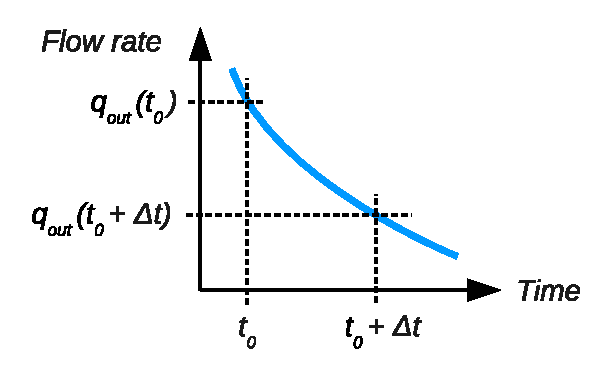
\includegraphics[width=0.75\columnwidth]{\figdir/recession.eps}
  \caption{Analysis of the recession following a flow peak. \label{fig:runConcParStor_recession}}
\end{figure}

When using \eqnref{eqn:runConcParStor_kEstim} to estimate the model parameters \strSurf{}, \strPref{}, \strInter{}, and \strBase{}, one must to take \eqnref{eqn:runConcParStor_retConstSurf}--\ref{eqn:runConcParStor_retConstBase} into account. Thus, the values of $k$ computed from \eqnref{eqn:runConcParStor_kEstim} have to be divided by the concentration time index \concTimeIndex{} in order to obtain the desired values of \strSurf{}, \strPref{}, \strInter{}, and \strBase{}.

In practice, the estimation of the storage constants is complicated by the fact that multiple runoff components contribute to stream flow at the same time. Thus, to estimate the value of a particular constant, one has to consider a recession which is likely to be \emph{dominated} by the corresponding process. For example, \strPref{} and possibly \strSurf{} (and possibly \strInter{}) are likely to control the steep part of the recession after major events. To identify \strBase{}, however, one needs analyze long-lasting recessions, preferably at the end of a rainy season. 

In general, the obtained values for \strSurf{}, \strPref{}, \strInter{}, and \strBase{} should be considered as rough estimates only. It is recommended to refine the estimates during calibration.

\chapter{Channel flow} \label{chap:chanFlow}
\renewcommand{\tabdir}{chapters/part_processes/channelFlow/tab}
\renewcommand{\figdir}{chapters/part_processes/channelFlow/fig}

\section{Introduction} \label{sec:chanFlow_intro}

This chapter desribes approaches to the simulation of open channel flow. In a dynamic model, we generally deal with unsteady flow conditions. One can distinguish between two basic concepts:

\begin{description}
  \item[Hydrodynamic approach] Such models are based on a solution of the St. Venant equations, expressing the conservation of momentum and mass. The solution of these (possibly simplified) partial differential equations requires rather expensive numerical methods.
  \item[Hydrological approaches] Such models still consider the principle of mass conservation (continuity equation). However, in contrast to hydrodynamic models, they do not account for the conservation of momentum or energy but rely on empirical relations between channel storage and flow.
\end{description}

In hydrological catchment models, hydrological approaches are widely because they are easier to implement and allow for fast computations based on anaytical solutions. Prominent examples include:
\begin{itemize}
  \item the single reservoir approach,
  \item the Muskingum method,
  \item the method of Kalinin-Miljukov (Nash's cascade).
\end{itemize}

The approach(es) described below apply to a single reach. Here, a reach is defined as a river section of a constant geometry (\ie{} cross-section and slope). In hydrological catchment modeling for larger areas, cross-section and slope data are usually scarce and a constant geometry is therefore assumed between the neighbored junctions along a river. Then, a reach is practically identical to the river section between two junctions.

%%%%%%%%%%%%%%%%%%%%%%%%%%%%%%%%%%%%%%%%%%%%%%%%%%%%%%%%%%%%%%%%%%%%%%%%%%%%%%%%
%%%%%%%%%%%%%%%%%%%%%%%%%%%%%%%%%%%%%%%%%%%%%%%%%%%%%%%%%%%%%%%%%%%%%%%%%%%%%%%%
%%%%%%%%%%%%%%%%%%%%%%%%%%%%%%%%%%%%%%%%%%%%%%%%%%%%%%%%%%%%%%%%%%%%%%%%%%%%%%%%

\section{Single reservoir approach} \label{sec:chanFlow_singleRes}

%%%%%%%%%%%%%%%%%%%%%%%%%%%%%%%%%%%%%%%%%%%%%%%%%%%%%%%%%%%%%%%%%%%%%%%%%%%%%%%%

\subsection{Processes and equations} \label{sec:chanFlow_singleRes_processes}

In this approach, a reach (\figref{fig:chanFlow_singleRes_reach}) is treated as a single reservoir. Considering the principle of mass conservation, the storage volume $v$ (\cbm) is related to the rates of inflow $q_{in}$ and outflow $q_{out}$ (both in \cbm/s) by the continuity equation \eqnref{eqn:chanFlow_singleRes_continuity_QinConst}.

\begin{equation} \label{eqn:chanFlow_singleRes_continuity_QinConst}
  \frac{dv}{dt} = q_{in} - q_{out}
\end{equation}

\begin{figure}
  \centering
  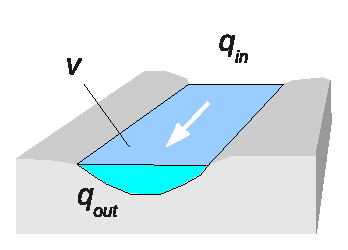
\includegraphics[width=0.6\columnwidth]{\figdir/reach.eps}
  \caption{Sketch of a reach with storage volume $v$, and the rates of in- and outflow ($q_{in}$, $q_{out}$). \label{fig:chanFlow_singleRes_reach}}
\end{figure}

To simulated the dynamics of $v$ for a given inflow rate, the continuity equation must be complemented by a second equation relating $q_{out}$ to $v$. In the case of a linear reservoir, for example, this missing relation is given by \eqnref{eqn:chanFlow_singleRes_outflowLinear} where $k$ is a retention constant with the dimension of a time. The advantage of this linear relation is that it allows for an analytical solution of \eqnref{eqn:chanFlow_singleRes_continuity_QinConst}.

\begin{equation} \label{eqn:chanFlow_singleRes_outflowLinear}
  q_{out}= \frac{1}{k} \cdot v
\end{equation}

Assuming that the inflow rate $q_{in}$ is constant over a discrete time step of length $\Delta t$, combining \eqnref{eqn:chanFlow_singleRes_continuity_QinConst} and \ref{eqn:chanFlow_singleRes_outflowLinear} and subsequent integration using the substitution method yields \eqnref{eqn:chanFlow_singleRes_linResSolution_QinConst}.

\begin{equation} \label{eqn:chanFlow_singleRes_linResSolution_QinConst}
  v(t_0 + \Delta t) =  (v(t_0) - q_{in} \cdot k) \cdot e^{(-\Delta t / k)} + q_{in} \cdot k
\end{equation}
\medskip
\begin{tabular}{lll}
  $v(t_0)$ & Initial storage at & L$^3$ \\
  $\Delta t$ & Length of time step & T \\
\end{tabular}

A slightly advanced version of the linear reservoir model is obtained if the inflow rate $q_{in}$ is allowed to vary linearly with time. Then, the modified continuity equation is given by \eqnref{eqn:chanFlow_singleRes_continuity_QinLinear}

\begin{equation} \label{eqn:chanFlow_singleRes_continuity_QinLinear}
  \frac{dv}{dt} = q_{in,0} + (q_{in,1} - q_{in,0}) \cdot t - q_{out}
\end{equation}

where $q_{in,0}$ and $q_{in,1}$ represent an initial and final inflow rate, respectively. After combining \eqnref{eqn:chanFlow_singleRes_continuity_QinLinear} with \eqnref{eqn:chanFlow_singleRes_outflowLinear}, the integration yields \eqnref{eqn:chanFlow_singleRes_linResSolution_QinLinear}

\begin{align} \label{eqn:chanFlow_singleRes_linResSolution_QinLinear}
  v(t_0 + \Delta t) =  & v(t_0) \cdot x + \frac{a \cdot (x-1)}{b^2} \\
                       & + \frac{q_{in,0} \cdot (x-1) - a \cdot \Delta t}{b} \nonumber
\end{align}

with the abbreviations

\begin{align*}
  a= & (q_{in,1} - q_{in,0}) / \Delta t \\ \nonumber
  b= & -1/k \\ \nonumber
  x= & e^{(-\Delta t / k)} \nonumber
\end{align*}

and

\begin{align*}
  q_{in,0} = q_{in}(t_0) \\ \nonumber
  q_{in,1} = q_{in}(t_0 + \Delta t) \nonumber
\end{align*}

This equation is also used in the LARSIM model \citep[same as Equation 3.54 in][]{Ludwig2006}.

Unfortunately, for natural channels, the relation between $q_{out}$ and $v$ is typically non-linear and  \eqnref{eqn:chanFlow_singleRes_outflowLinear} is therefor not applicable. However, the analytical solution of the linear reservoir equation (\eqnsref{eqn:chanFlow_singleRes_linResSolution_QinConst} or \ref{eqn:chanFlow_singleRes_linResSolution_QinLinear}) is very attractive to use because of its low computational cost. A common solution to this problem is the idea of a locally-linear reservoir. In this concept, the analytical solution of the linear reservoir equation is still used but the retention constant $k$ is allowed to depend on the storage volume $v$ (or the outflow rate $q_{out}$).

According to \eqnref{eqn:chanFlow_singleRes_outflowLinear}, the retention constant of a linear reservoir is given by \eqnref{eqn:chanFlow_singleRes_retConst_trueLinear}

\begin{equation} \label{eqn:chanFlow_singleRes_retConst_trueLinear}
 k = \frac{v}{q_{out}}
\end{equation}
.

Similarly, for the locally-linear reservoir, the retention constant is given by \eqnref{eqn:chanFlow_singleRes_retConst_locallyLinear}

\begin{equation} \label{eqn:chanFlow_singleRes_retConst_locallyLinear}
 k = \frac{\Delta v}{\Delta q_{out}}
\end{equation}
.

Thus, the retention constant $k$ still equals the slope of the relation between $v$ and $q_{out}$  (\figref{fig:chanFlow_singleRes_dVdQ}).

\begin{figure}
  \centering
  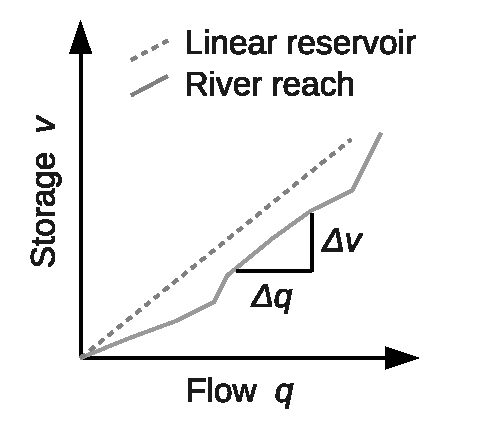
\includegraphics[width=0.5\columnwidth]{\figdir/dVdQ.eps}
  \caption{Relation between storage volume $v$ and outflow rate $q_{out}$ for a linear reservoir and a river reach. \label{fig:chanFlow_singleRes_dVdQ}}
\end{figure}

For channels of known geometry, the relation between $q_{out}$ to $v$ (\figref{fig:chanFlow_singleRes_dVdQ}) can be derived from a rating curve, \ie{} corresponding observations of flow rates and water levels (the latter being convertable to storage volumes). Since the vast majority of simulated reaches in a hydrological model is ungaged, rating curves are not practically available and need to be estimated. This is usually done by applying Manning's equation (\eqnref{eqn:chanFlow_singleRes_manning}).

\begin{equation} \label{eqn:chanFlow_singleRes_manning}
  q(h)= \frac{1}{n} \cdot \sqrt{S_f} \cdot R(h)^{2/3} \cdot A(h)
\end{equation}
\medskip
\begin{tabular}{lll}
  $q$ & Flow rate & \cbm/s \\
  $S_f$ & Slope of the energy grade line & -- \\
  $R$ & Hydraulic radius &  m \\
  $A$ & Wet cross-section area & \sqm \\
  $h$ & Water level & m \\
  $n$ & Manning's $n$ (parameter) & Non-physical \\
\end{tabular}

Considering that the storage volume $v$ in a uniform reach equals $A \cdot L$ ($L$: length of the channel), \eqnref{eqn:chanFlow_singleRes_manning} can be used to tabulate corresponding pairs of $v$ and $q_{out}$ and thus also $k(q_{out})$ or $k(v)$, respectively (recall \eqnref{eqn:chanFlow_singleRes_retConst_locallyLinear}). The required information are:
\begin{itemize}
  \item The functions $A(h)$ and $R(h)$. They can easily be computed from the x-section's geometry (table of offsets and corresponding elevations).
  \item The roughness parameter $n$. Tables and empirical formulas exist to estimate this value from channel properties. It can also be fitted by steady flow modeling.
  \item The slope of the energy grade line $S_f$. In practice, only the slope of the channel bottom $S_0$ is constant and known. It can be measured in the field or has to be gathered from a digital elevation model (with subsequent quality checks).
\end{itemize}

%%%%%%%%%%%%%%%%%%%%%%%%%%%%%%%%%%%%%%%%%%%%%%%%%%%%%%%%%%%%%%%%%%%%%%%%%%%%%%%%

\subsection{Mathematical solution} \label{sec:chanFlow_singleRes_solution}

\subsubsection*{Governing equation}

In each time step, the storage $v$ is updated using \eqnref{eqn:chanFlow_singleRes_linResSolution_QinLinear}. The applied retention constant is an average value ($\overline{k}$) taking into account the initial storage volume, the initial inflow rate, and the inflow rate at the end of the time step (\eqnref{eqn:chanFlow_singleRes_averageK})

\begin{equation} \label{eqn:chanFlow_singleRes_averageK}
  \overline{k} = \frac{k(q_{in}(t_0)) + k(q_{in}(t_0 + \Delta t)) + k(v(t_0))}{3}
\end{equation}

with all $k$ values taken from the $\Delta v/\Delta q$ relation (\eqnref{eqn:chanFlow_singleRes_retConst_locallyLinear}).

To apply \eqnsref{eqn:chanFlow_singleRes_linResSolution_QinLinear} and \ref{eqn:chanFlow_singleRes_averageK}, the inflow rates corresponding to the begin and the end of a time step, $q_{in}(t_0)$ and $q_{in}(t_0 + \Delta t)$, must be known.

\subsubsection*{Inflow rates}

Problems with conservation of mass may arise from using $q_{in}(t_0)$ and $q_{in}(t_0 + \Delta t)$ together with the assumption of a linear variation over $\Delta t$ when simulating multiple reaches in series. This is due to the fact that the outflow from a reach -- and thus the inflow of the downstream reach -- varies exponentially rather than linearly (see \eqnref{eqn:chanFlow_singleRes_linResSolution_QinConst} \& \ref{eqn:chanFlow_singleRes_linResSolution_QinLinear}). To allow for a proper mass balance (priority) while also taking into account the variation in the inflow rate (secondary objective), the model uses as input
\begin{enumerate}
  \item the rate at the end of the time step, $q_{in}(t_0 + \Delta t)$.
  \item the average inflow rate for the time step, $\overline{q_{in}}$.
\end{enumerate}

Then, the inflow rate at the begin of the time step, $q_{in}(t_0)$ is estimated from these two values using
\begin{equation*}
q_{in}(t_0)= max(0., 2 \cdot \overline{q_{in}} - q_{in}(t_0 + \Delta t))
\end{equation*}
and subsequently applying the correction
\begin{equation*}
q_{in}(t_0 + \Delta t)= 2 \cdot \overline{q_{in}} - q_{in}(t_0)
\end{equation*}
The latter correction is necessary to account for the mass balance in those cases where the \second{} argument of $max()$ is negative and $q_{in}(t_0)$ is therefor set to zero. These are cases where the value of the average inflow rate is incompatible with the assumption of a linear variation over $\Delta t$.

\subsubsection*{Outflow rates}

Using the concept of the linear reservoir, the outflow rate at the end of the time step is computed from \eqnref{eqn:chanFlow_singleRes_outflowEnd}.

\begin{equation} \label{eqn:chanFlow_singleRes_outflowEnd}
  q_{out}(t_0 + \Delta t)= \frac{1}{\overline{k}} \cdot v(t_0 + \Delta t)
\end{equation}

The time-step averaged outflow rate is calculated using \eqnref{eqn:chanFlow_singleRes_outflowAvg}, which is a discrete version of the mass balance equation.

\begin{equation} \label{eqn:chanFlow_singleRes_outflowAvg}
\overline{q_{out}}= \frac{v(t_0) - v(t_0 + \Delta t)}{\Delta t} + \overline{q_{in}}
\end{equation}

%%%%%%%%%%%%%%%%%%%%%%%%%%%%%%%%%%%%%%%%%%%%%%%%%%%%%%%%%%%%%%%%%%%%%%%%%%%%%%%%

\subsection{Hints for application} \label{sec:chanFlow_singleRes_hints}

In hydrological catchment modeling, data on the geometry of river cross-sections are usually scarce. The \software{topocatch} software \citep{Echse-Tools-Doc} contains methods to estimate the x-section characteristics for all reaches in a river basin using survey data from a limited number of sites only. Basically, these methods perform a spatial regionalization of the functions $A(h)$ and $R(h)$. It then applies \eqnref{eqn:chanFlow_singleRes_manning} to generate a table of corresponding storage volumes and outflow rates, allowing for look-up of the retention constant (\eqnref{eqn:chanFlow_singleRes_retConst_locallyLinear}).

\chapter{Evaporation from Water Surfaces} \label{chap:evap}
\renewcommand{\tabdir}{chapters/part_processes/evaporation/tab}
\renewcommand{\figdir}{chapters/part_processes/evaporation/fig}

\section{Introduction} \label{sec:evap_intro}

This chapter introduces evaporation models. The approach(es) can be used to estimate the water losses associated with evaporation from lake, reservoir, and river surfaces.

%%%%%%%%%%%%%%%%%%%%%%%%%%%%%%%%%%%%%%%%%%%%%%%%%%%%%%%%%%%%%%%%%%%%%%%%%%%%%%%%
%%%%%%%%%%%%%%%%%%%%%%%%%%%%%%%%%%%%%%%%%%%%%%%%%%%%%%%%%%%%%%%%%%%%%%%%%%%%%%%%
%%%%%%%%%%%%%%%%%%%%%%%%%%%%%%%%%%%%%%%%%%%%%%%%%%%%%%%%%%%%%%%%%%%%%%%%%%%%%%%%

\section{Makkink model} \label{sec:evap_makkink}

The Makkink model is a simple empirical equation to estimate evaporation using a minimum set of input data, namely short wave radiation and air temperature. In has been derived for the Netherlands. Using convenient units, the basic equation is (\eqnref{eqn:evap_makkink_main})

\begin{equation} \label{eqn:evap_makkink_main}
  e = c \cdot \frac{s}{s + \gamma} \cdot \frac{\radShortwaveIn}{1000 \cdot \evapHeatWater \cdot \densityWater} + b
\end{equation}

with

\begin{tabular}{lp{0.8\columnwidth}}
  $e$ & Makkink reference evaporation (m/s) \\
  $s$ & Slope of the curve of saturation water vapor pressure (kPa / K) \\
  $\gamma$ & Psychrometric constant (kPa / K) \\
  $\radShortwaveIn$ & Incoming short-wave radiation (W/\sqm{}) \\
  $\evapHeatWater$ & Latent heat of water evaporation (kJ/kg). \\
  $\densityWater$ & Density of water ($\approx$ 1000 kg/\cbm{}). \\
  $c$ & Empirical factor (--). \\
  $b$ & Empirical correction term (m/s). \\
\end{tabular}

\medskip
One should realize that only the incoming short-wave radiation is used in \eqnref{eqn:evap_makkink_main}, thus other terms of the energy balance, such as reflection (albedo), long wave emissions, and heat storage are all neglected.

For the dimensionless term $s/(s + \gamma)$ \citet{Yao2009} present a convenient approximation based on the air temperature \airtemp{} in units of \celsius{}  (\eqnref{eqn:evap_makkink_dimlessFraction}). The error from using this approximation is < 4~\% for temperatures between 4 and 30~\celsius{} and about 7~\% at 0~\celsius{} when compared to the equations for separate estimation of $s$ and $\gamma$ given in \citet{Hiemstra2011}.

\begin{equation} \label{eqn:evap_makkink_dimlessFraction}
  \frac{s}{s + \gamma} \approx 0.439 + 0.01124 \cdot \airtemp
\end{equation}

The latent heat of water evaporation \evapHeatWater{} (kJ/kg) can be estimated from the water temperature $T$ (\celsius) using \eqnref{eqn:evap_makkink_evapHeatWater} \citep{Hiemstra2011}. Since water temperature data are usually unavailable, the air temperature \airtemp{} must be used as a substitute for $T$.

\begin{equation} \label{eqn:evap_makkink_evapHeatWater}
  \evapHeatWater = 2501 - 2.375 \cdot T
\end{equation}

For the two empirical parameters, \citet{Winter1995} report values of $c= 0.61$ and $b=-0.012/100/86400$ (unit of $b$ converted from cm/d to m/s). \citet{Hiemstra2011} suggest $c = 0.65$ and $b = 0$ but their report does not explicitly focus on evaporation from water surfaces.

\tabref{tab:evap_makkink_example} provides some results of the application of \eqnref{eqn:evap_makkink_main} for selected temperatures and short-wave radiation inputs.

\begin{table}
  \caption[Makkink evaporation for different values of temperature and daily-average short-wave radiation.]{Makkink evaporation (mm/day) for different values of temperature (\celsius{}) and daily-average short-wave radiation (W/\sqm). The empirical parameters were set to $c=0.61$ and $b=-0.012/100/86400$.  \label{tab:evap_makkink_example}}
  \centering
  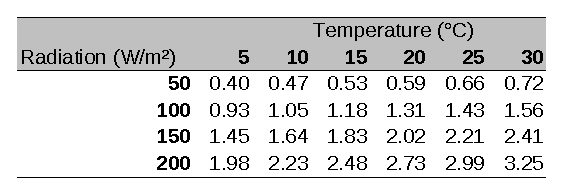
\includegraphics[width=0.9\columnwidth]{\figdir/makkink.eps}
\end{table}

\chapter{Evapotranspiration} \label{chap:et}
\renewcommand{\tabdir}{chapters/part_processes/evapotranspiration/tab}
\renewcommand{\figdir}{chapters/part_processes/evapotranspiration/fig}

\section{Introduction} \label{sec:et_intro}

This chapter describes approaches to model evapotranspiration. The focus is on very simple approaches relying on a two-step calculation procedure:
\begin{enumerate}
  \item Computation of a \emph{potential} evapotranspiration rate \etPot. This represents the maximum possible rate in the absence of water stress. It is basically limited by energy supply.
  \item Estimation of the \emph{actual} evapotranspiration rate \etReal{} from the potential rate taking into account the properties of vegetation and the limitation by a soil moisture deficit.
\end{enumerate}

%%%%%%%%%%%%%%%%%%%%%%%%%%%%%%%%%%%%%%%%%%%%%%%%%%%%%%%%%%%%%%%%%%%%%%%%%%%%%%%%
%%%%%%%%%%%%%%%%%%%%%%%%%%%%%%%%%%%%%%%%%%%%%%%%%%%%%%%%%%%%%%%%%%%%%%%%%%%%%%%%
%%%%%%%%%%%%%%%%%%%%%%%%%%%%%%%%%%%%%%%%%%%%%%%%%%%%%%%%%%%%%%%%%%%%%%%%%%%%%%%%

\section{Potential evapotranspiration} \label{sec:et:pot}

\section{Hargreaves model} \label{sec:et:pot:hargreaves}

This is a very simply model yielding estimates of \etPot{} with daily resolution. It requires as input
\begin{itemize}
  \item Incoming short-wave radiation
  \item Daily minimum and maximum temperature
\end{itemize}

If the radiation is given as a daily average value (instead of a sum), the Hargreaves model takes the form of \eqnref{eqn:et:pot:hargreaves}

\begin{align} \label{eqn:et:pot:hargreaves}
  \etPot = & CH \cdot \left( \frac{t_{max}+t_{min}}{2} + CT \right) \cdot \\
           & \sqrt{t_{max}-t_{min}} \cdot 0.0864 \cdot \radShortwaveIn{} \nonumber
\end{align}

with

\medskip
\begin{tabular}{p{0.25\columnwidth}p{0.55\columnwidth}}
  \etPot & Hargreaves potential evapotranspiration rate (mm/day) \\
  $t_{max}$, $t_{min}$ & Daily minimum and maximum of air temperature (\celsius) \\
  \radShortwaveIn{} & Daily average of incoming short-wave radiation (W/\sqm{}) \\
  0.0864 & Factor to convert \radShortwaveIn{} from W/\sqm{} into MJ/\sqm{}/day \\
  $CH$ & Empirical coefficient, $CH$= 0.0023 \\
  $CT$ & Empirical coefficient, $CT$= 17.8 \\
\end{tabular}


\section{Makkink model} \label{sec:et:pot:makkink}

The Makkink model is another simple approach to estimate potential evaporation using only temperature and downward short-wave radiation as predictors. The approach is discussed in detail by \citet{deBruin1987, Feddes1987, Hiemstra2011}.

Using convenient units, the basic equation without an additive empirical constant \citep[see][]{deBruin1987} is \eqnref{eqn:et:pot:makkink}

\begin{equation} \label{eqn:et:pot:makkink}
  \etPot = c \cdot \frac{s}{s + \gamma} \cdot \frac{\radShortwaveIn}{1000 \cdot \evapHeatWater \cdot \densityWater}
\end{equation}

with

\medskip
\begin{tabular}{lp{0.8\columnwidth}}
  \etPot & Makkink reference crop-evaporation (m/s) \\
  $s$ & Slope of the curve of saturation water vapor pressure (kPa / K) \\
  $\gamma$ & Psychrometric constant (kPa / K) \\
  $\radShortwaveIn$ & Incoming short-wave radiation (W/\sqm{}) \\
  $\evapHeatWater$ & Latent heat of water evaporation (kJ/kg) \\
  $\densityWater$ & Density of water ($\approx$ 1000 kg/\cbm{}) \\
  $1000$ & Factor to convert kJ into J \\
  $c$ & Dimensionless empirical constant, $c$=0.65 \\
\end{tabular}


The latent heat of water evaporation \evapHeatWater{} (kJ/kg) is simply a function of temperature (see \eqnref{eqn:evap_makkink_evapHeatWater} on page~\pageref{eqn:evap_makkink_evapHeatWater}). For the dimensionless term $s/(s + \gamma)$ \citet{Yao2009} present a convenient approximation based on the air temperature (see \eqnref{eqn:evap_makkink_dimlessFraction} on page~\pageref{eqn:evap_makkink_dimlessFraction}). A more accurate estimate is obtained, however, using the empirical expressions for $s$ and $\gamma$ (both in hPa/K) from \eqnref{eqn:slopeSatVapPress} and \eqnref{eqn:psychroConst}

\begin{align} 
  s=& 6.11 \cdot exp\left(\frac{17.3 \cdot \airtemp}{237.3 + \airtemp} \right) \cdot \label{eqn:slopeSatVapPress} \\
    & \frac{4105.3}{(237.3 + \airtemp)^2} \nonumber \\
  \gamma=& 0.016286 \cdot \frac{\airPressure}{\evapHeatWater(\airtemp)} \label{eqn:psychroConst}
\end{align}

where \airPressure{} is the air pressure (hPa) and \airtemp{} is the air temperature  in \celsius{} \citep{Dyck1995}.

%%%%%%%%%%%%%%%%%%%%%%%%%%%%%%%%%%%%%%%%%%%%%%%%%%%%%%%%%%%%%%%%%%%%%%%%%%%%%%%%
%%%%%%%%%%%%%%%%%%%%%%%%%%%%%%%%%%%%%%%%%%%%%%%%%%%%%%%%%%%%%%%%%%%%%%%%%%%%%%%%
%%%%%%%%%%%%%%%%%%%%%%%%%%%%%%%%%%%%%%%%%%%%%%%%%%%%%%%%%%%%%%%%%%%%%%%%%%%%%%%%

\section{Real evapotranspiration} \label{sec:et:real}

In the approaches described here, the rate of real evapotranspiration \etReal{} is computed by multiplying the potential rate \etPot{} with dimensionless correction factors. Typically, these factors account for
\begin{itemize}
  \item the different transpiration characteristics of the actual vegetation as compared to the reference vegetation to which \etPot{} refers (usually short grass). These factors are known as \emph{crop factors} (\secref{sec:et:real:cropfactors}).
  \item the reduction of plant transpiration due to soil moisture limitation (\secref{sec:et:real:soilmoisture}).
\end{itemize}

\subsection{Crop factors} \label{sec:et:real:cropfactors}

For some equations to estimate \etPot{}, an extensive set of crop factors has been established based on empirical research. The values vary between different crops and also account for the different stages of plant grow, \ie{} seasonality. For the Makkink model (\secref{sec:et:pot:makkink}), crop factors can be found in \citet{Feddes1987}. For wider applicability, it is desireable to derive the crop factors from other easily available data. A potential candidate is the leaf-area index \leafAreaIndex. Based on figure \figref{fig:et:real:cropfactor-LAI}, an approximate relation between the crop factor of the Makkink model and the \leafAreaIndex{} can be derived (\eqnref{eqn:et:real:cropfactor-LAI}).

\begin{equation} \label{eqn:et:real:cropfactor-LAI}
  \text{crop factor} \approx 0.14 \cdot \leafAreaIndex + 0.4 
\end{equation}

Note that, following the conventional definition of \etPot{}, the crop factor should take a value of one for the reference crop (typically actively growing gras of 12~cm height with unlimited water supply). Assuming that the corresponding \leafAreaIndex{} is about 5 \citep[see, \eg][]{Misra1981} or \citep[][page 11]{Bremicker2006}, the simplest linear approach would be \eqnref{eqn:et:real:cropfactor-LAI-simple}.

\begin{equation} \label{eqn:et:real:cropfactor-LAI-simple}
  \text{crop factor} \approx 0.2 \cdot \leafAreaIndex
\end{equation}

This equation, however, implies that evapotranspiration from bare soil is zero. In reality, a non-zero intercept is more plausible.

During calibration of a hydrological model for the Upper Neckar Basin (Germany), the relation shown in \eqnref{eqn:et:real:cropfactor-LAI-Neckar} was identified. It yielded the best result for a larger part of the catchment (gage Kirchtellinsfurt, 2300~\sqkm). The optimum parameters for smaller sub-basins were similar. The assumed \leafAreaIndex{} of grassland vegetation in that model was 5.

\begin{equation} \label{eqn:et:real:cropfactor-LAI-Neckar}
  \text{crop factor} \approx 0.16 \cdot \leafAreaIndex + 0.2 
\end{equation}



\begin{figure}
  \centering
  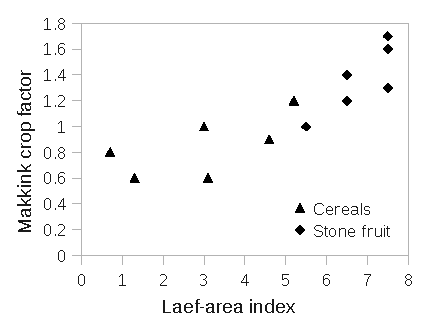
\includegraphics[width=0.75\columnwidth]{\figdir/cropfactor_LAI.eps}
  \caption[Relation between the crop factor (for Makkink model) and the leaf-area index (\sqm/\sqm) for two selected crops.]{Relation between the crop factor (for Makkink model) and the leaf-area index (\sqm/\sqm) for two selected crops. Crop factors and the corresponding values of \leafAreaIndex{} were taken from \citet{Feddes1987} and \citet{Ludwig2006}, respectively. \label{fig:et:real:cropfactor-LAI}}
\end{figure}

\subsection{Influence of soil moisture} \label{sec:et:real:soilmoisture}

A widely used scheme to account for the limitation of real evapotranspiration by soil moisture is illustrated in \figref{fig:et:real:soilmoisture}. This approach uses two empirical constants $rs_{et min}$ and $rs_{et max}$ representing threshold values of relative soil saturation. For very dry soil with relative saturation between 0 and $rs_{et min}$, real evapotranspiration is zero. For wet conditions with relative saturation between $rs_{et max}$ and 1, the rate of real evapotranspiration \etReal{} is equal to the potential rate \etPot{}. For intermediate conditions, \etReal{} is assumed to vary linearily with soil saturation (\ie{} soil moisture). Mathematically, this is expressed by \eqnref{eqn:et:real:soilmoisture}.

\begin{equation} \label{eqn:et:real:soilmoisture}
  \frac{\etReal}{\etPot} = min\left(1, max\left(0, \frac{rs-rs_{et min}}{rs_{et max}-rs_{et min}} \right)\right)
\end{equation}

\begin{figure}
  \centering
  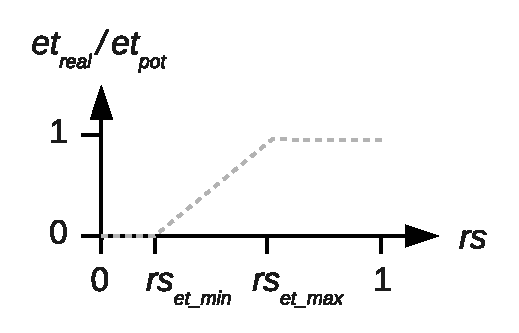
\includegraphics[width=0.6\columnwidth]{\figdir/soilMoistureEffect.eps}
  \caption{Ratio of real to potential evapotranspiration \etReal/\etPot{} as a function of relative soil saturation $rs$. \label{fig:et:real:soilmoisture}}
\end{figure}

In this definition, the relative soil saturation $rs$ is the quotient of the current soil water content $\soilWaterContent$ and the soil-specific maximum value $\soilWaterContentMax$. Thus, the two parameters $rs_{et min}$ and $rs_{et max}$ take values in range 0 to 1. A reasonable estimate for $rs_{et min}$ can be obtained from data on the water content at the wilting point. This value varies considerably between soil types as illustrated in \figref{fig:et:real:pFCurve}.

\begin{figure}
  \centering
  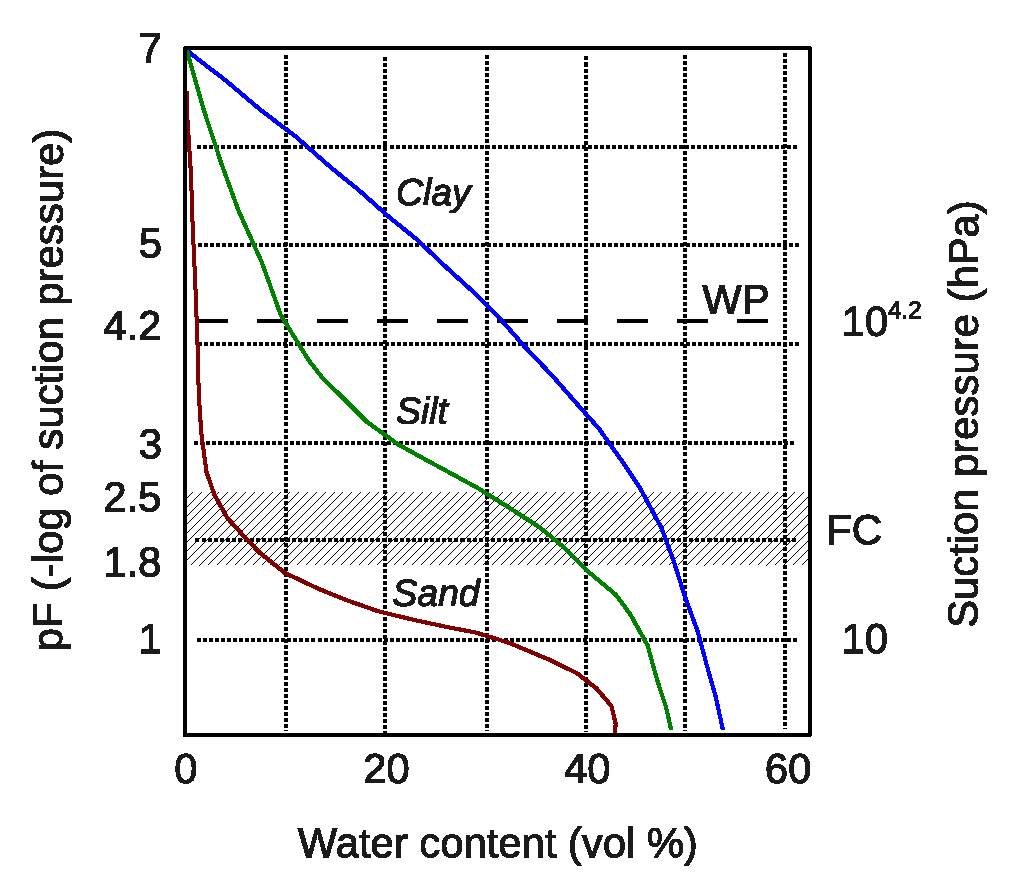
\includegraphics[width=0.9\columnwidth]{\figdir/pF_and_waterContent.eps}
  \caption{Typical relation between water content and suction pressure for different soil types. The permanent wilting point is defined as pF=4.2 ($\approx$ 1500 kPa). The hatching marks the typical range of the field capacity found in soils. Adapted from \citet{Scheffer1998}. \label{fig:et:real:pFCurve}}
\end{figure}

Some characteristic values of soil water content (based on \figref{fig:et:real:pFCurve}) and the corresponding estimates of model parameters are presented in \tabref{tab:et:real:soilmoisture}.

\begin{table}
  \caption{Characteristic values of the soil water content $\soilWaterContent$ and corresponding estimates of model parameters derived from \figref{fig:et:real:pFCurve}. \label{tab:et:real:soilmoisture}}
  {\small
  \begin{tabular}{|rlllll|} \hline
    \rowcolor[gray]{0.9}
         &                        & $\soilWaterContent$ at & $\soilWaterContent$ at & & \\
    \rowcolor[gray]{0.9}
    Soil & $\soilWaterContentMax$ & pF=2.5 & pF=4.2 & $rs_{et max}$ & $rs_{et min}$ \\ \hline
    Sand & 0.43 & 0.03 & 0.02 & < 0.07 & 0.05 \\
    Silt & 0.48 & 0.3  & 0.1  & < 0.63 & 0.21 \\
    Clay & 0.53 & 0.46 & 0.32 & < 0.86 & 0.6 \\
  \hline
  \end{tabular} 
  }
\end{table}

\chapter{Storage in lakes and reservoirs} \label{chap:resStor}
\renewcommand{\tabdir}{chapters/part_processes/reservoirStorage/tab}
\renewcommand{\figdir}{chapters/part_processes/reservoirStorage/fig}

\section{Introduction} \label{sec:resStor_intro}

This chapter desribes approaches to the simulation of water storage in reservoirs. In a wider sense, the term \emph{reservoir} includes natural lakes and the various types of operated reservoirs.

%%%%%%%%%%%%%%%%%%%%%%%%%%%%%%%%%%%%%%%%%%%%%%%%%%%%%%%%%%%%%%%%%%%%%%%%%%%%%%%%
%%%%%%%%%%%%%%%%%%%%%%%%%%%%%%%%%%%%%%%%%%%%%%%%%%%%%%%%%%%%%%%%%%%%%%%%%%%%%%%%
%%%%%%%%%%%%%%%%%%%%%%%%%%%%%%%%%%%%%%%%%%%%%%%%%%%%%%%%%%%%%%%%%%%%%%%%%%%%%%%%

\section{Storage in uncontrolled lakes} \label{sec:resStor_lake}

%%%%%%%%%%%%%%%%%%%%%%%%%%%%%%%%%%%%%%%%%%%%%%%%%%%%%%%%%%%%%%%%%%%%%%%%%%%%%%%%

\subsection{Processes and equations} \label{sec:resStor_lake_processes}

The fundamental principle for the simulation of lake storage is expressed by the mass balance equation (\eqnref{eqn:resStor_lake_massBalancePure}).

\begin{equation} \label{eqn:resStor_lake_massBalancePure}
  \frac{dv}{dt} = q_{in} + p - q_{out} - e
\end{equation}

\begin{tabular}{lll}
  $v$ & Storage volume & L$^3$ \\
  $q_{in}$ & Inflow rate & L$^3$/T \\
  $q_{out}$ & Outflow rate & L$^3$/T \\
  $p$ & Precipitation flux & L$^3$/T \\
  $e$ & Evaporation flux & L$^3$/T \\
\end{tabular}

\medskip
For a natural lake with a single outflow, the outflow rate is related to the lake's water level $h$ through a rating curve $Q_{out}(h)$ (\figref{fig:resStor_lake_massBalance}). Furthermore, the water level $h$ is related to the storage volume $v$ by the storage curve $H(v)$. The latter represents the lake's bathymetry, \ie{} the topography of the bottom. Sometimes, the rating curve and the storage curve may be represented by analytical functions, typically using power equations or polynomials, respectively. In practice, however, lookup tables generally allow for greater flexibility as compared to analytical expressions.

\begin{figure}
  \centering
  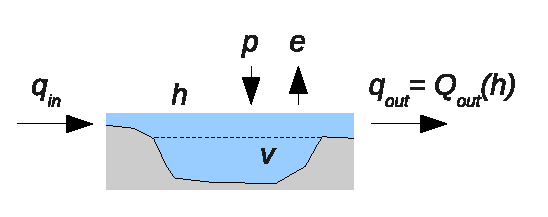
\includegraphics[width=0.7\columnwidth]{\figdir/balance.eps}
  \caption[Side view of a lake with uncontrolled outflow through an outlet channel.]{Side view of a lake with uncontrolled outflow through an outlet channel. Symbols as in \eqnref{eqn:resStor_lake_massBalancePure}. \label{fig:resStor_lake_massBalance}}
\end{figure}

The rates of precipitation and evaporation fluxes are obtained by multiplying the corresponding rates (dimension L/T) with an appropriate value of the lake's surface area (\eqnref{eqn:resStor_lake_fluxP} \& \ref{eqn:resStor_lake_fluxE}).

\begin{align}
p= & P \cdot a_{max}  \label{eqn:resStor_lake_fluxP} \\
e= & E \cdot A(H(v))  \label{eqn:resStor_lake_fluxE}
\end{align}

\begin{tabular}{lp{0.5\columnwidth}l}
  $P$ & Intensity of precipitation & L/T \\
  $E$ & Rate of evaporation & L/T \\
  $a_{max}$ & Maximum extent of the lake's surface area & L$^2$ \\
  $A(h)$ & Surface area as a function of water level $h$ & L$^2$ \\
\end{tabular}

\medskip
The reasons for using different values of the surface area in the calculation of precipitation and evaporation fluxes are as follows:
\begin{itemize}
  \item If a constant surface area would be used in \eqnref{eqn:resStor_lake_fluxE}, this would no longer be a continuous function. As long as the there was some water in the lake, the evaporation flux would be $>0$. But as soon as the last amount of liquid water has vanished, the flux becomes zero. Such a discontinuity is problematic when solving the differential equation \eqnref{eqn:resStor_lake_massBalancePure}. The choice of a \emph{continuous} function $A(h)$ resolves this problem, as it makes the evaporation flux $E$ decrease gradually, as the storage volume approaches zero.
  \item In reality, the lake's surface area being exposed to precipitation is variable too, as expressed by $A(h)$. However, in hydrological catchment models, the area of \emph{land surfaces} is typically constant. Therefore, to avoid mass balance errors, the lake's surface area is taken as constant too. The maximum extent of the lake $a_{max}$ is a natural choice. Effectively, rain falling on possibly dry parts of the bottom still contributes to the lake's storage volume.
\end{itemize}

Using the rating curve $Q_{out}(h)$ and the storage curve $H(v)$ as well as the definitions from \eqnref{eqn:resStor_lake_fluxP} and \ref{eqn:resStor_lake_fluxE}, the mass balance (\eqnref{eqn:resStor_lake_massBalancePure}) can be rewritten as \eqnref{eqn:resStor_lake_massBalanceExt}.

\begin{equation} \label{eqn:resStor_lake_massBalanceExt}
  \frac{dv}{dt} = q_{in} + P \cdot a_{max} - Q_{out}(H(v)) - E \cdot A(H(v))
\end{equation}

%%%%%%%%%%%%%%%%%%%%%%%%%%%%%%%%%%%%%%%%%%%%%%%%%%%%%%%%%%%%%%%%%%%%%%%%%%%%%%%%

\subsection{Mathematical solution} \label{sec:resStor_lake_solution}

\subsubsection*{Strategy}
The two functions $Q_{out}(H(v))$ and $A(H(v))$ at the right hand side of \eqnref{eqn:resStor_lake_massBalanceExt} may be arbitrarily complicated. Moreover, the functions are typically available as lookup tables rather than analytical expressions. Therefore, \eqnref{eqn:resStor_lake_massBalanceExt} has to be solved numerically. To obtain accurate and stable (\ie{} positive) solutions, an ODE solver with automatic time-step adjustment must be used.

\subsubsection*{Inflow rates}
The currently used implementation allows for a linear variation of the inflow rate within a discrete modeling time step of length $\Delta t$. As input, the time-step averaged inflow rate $\overline{q_{in}}$ and the instantaneous rate at the end of the time step $q_{in}(t_0 + \Delta t)$ are used. The missing rate at the begin of the time step $q_{in}(t_0)$ is estimated as described in \secref{sec:chanFlow_singleRes_solution} (page~\pageref{sec:chanFlow_singleRes_solution}).

\subsubsection*{Outflow rates}
The numerical solution of \eqnref{eqn:resStor_lake_massBalanceExt} yields the storage volume at the end of a modeling time step and the corresponding outflow rate $q_{out}(t_0 + \Delta t)$ is obtained from the combined rating curve and storage curve $Q_{out}(H(v))$.

An accurate time-step averaged outflow rate $\overline{q_{out}}$ is calculated from a discrete version of the mass balance equation (\eqnref{eqn:resStor_lake_outflowAvg}).

\begin{equation} \label{eqn:resStor_lake_outflowAvg}
  \overline{q_{out}}= \frac{v(t_0) - v(t_0 + \Delta t)}{\Delta t} + \overline{q_{in}} + \frac{vp}{\Delta t} - \frac{ve}{\Delta t}
\end{equation}

Here, $vp$ and $ve$ represent the total volumes of precipitation input and evaporation losses within a single time step, respectively. Both $vp$ and $ve$ are treated as state variables which are initialized to zero at the beginning of a time step ($t_0$). This approach allows for the computation of a proper mass balance even if the rates of precipitation or evaporation are variable over $\Delta t$. Currently, this is only the case for evaporation, since the flux is dependend on the storage (see \eqnref{eqn:resStor_lake_fluxE}).

%%%%%%%%%%%%%%%%%%%%%%%%%%%%%%%%%%%%%%%%%%%%%%%%%%%%%%%%%%%%%%%%%%%%%%%%%%%%%%%%

\subsection{Implementation} \label{sec:resStor_lake_implementation}

\tabref{tab:resStor_lake_implementation} relates the identifier names used in the model implementation (names of state variables, parameters, inputs, and outputs) to the symbols used in the process equations (\secref{sec:resStor_lake_processes}). Note that this table does not list external input variables used in the calculation of the rate of evaporation (symbol $E$ in \eqnref{eqn:resStor_lake_fluxE}). Modeling concepts for evaporation can be found in \chapref{chap:evap}.

\begin{table*}
\caption{Symbols used in the process equations (\secref{sec:resStor_lake_processes}) and corresponding identifiers. \label{tab:resStor_lake_implementation}}
\begin{tabular}{|p{0.2\textwidth}p{0.13\textwidth}p{0.07\textwidth}p{0.42\textwidth}|}  \hline
\rowcolor[gray]{0.9}
Symbol & Identifier & Units & Details \\ \hline
\multicolumn{4}{|c|}{\textit{State variables}} \\
$v$ & \verb!v! & \cbm{} & Storage volume \\
$vp$ & \verb!vp! & \cbm{} & Total volume of precipitation in a single time step \\
$ve$ & \verb!ve! & \cbm{} & Total evaporated volume in a single time step \\ \hline
\multicolumn{4}{|c|}{\textit{Simulated inputs}} \\
$\overline{q_{in}}$ & \verb!qi_avg! & \cbm{}/s & Inflow rate (time-step average) \\
$q_{in}(t_0 + \Delta t)$ & \verb!qi_end! & \cbm{}/s & Inflow rate (value at end of time-step) \\  \hline
\multicolumn{4}{|c|}{\textit{Scalar parameters (object-specific)}} \\
$a_{max}$ & \verb!area_max! & \sqm{} & Maximum surface area \\  \hline
\multicolumn{4}{|c|}{\textit{Parameter functions (object-specific)}} \\
$H(v)$ & \verb!v2h! & m & Storage curve (tabulated function) \\
$A(h)$ & \verb!h2a! & \sqm{} & Area curve to compute evaporation loss (tabulated function) \\
$Q_{out}(h)$ & \verb!h2q! & \sqm{} & Rating curve at lake outlet (tabulated function) \\  \hline
\multicolumn{4}{|c|}{\textit{Outputs}} \\
$\overline{q_{out}}$ & \verb!qx_avg! & \cbm{}/s & Outflow rate (time-step average) \\
$q_{out}(t_0 + \Delta t)$ & \verb!qx_end! & \cbm{}/s & Outflow rate (value at end of time-step) \\
$h$ & \verb!h! & m & Water level \\ \hline
\end{tabular}
\end{table*}


%%%%%%%%%%%%%%%%%%%%%%%%%%%%%%%%%%%%%%%%%%%%%%%%%%%%%%%%%%%%%%%%%%%%%%%%%%%%%%%%

\section{Notes on input data} \label{sec:resStor_inputs}

In real-world model applications, the required functions $H(v)$, $Q_{out}(h)$, and $A(h)$ are often not known but have to be estimated. Some recommendations are given in the sub-sections below.

\subsection{Storage curve}
Sometimes, information on the lake's bathymetry are available from topographic maps as lines of equal depth. Via the steps of digitizing and vector-to-raster conversion, a digital elevation model (DEM) of the lake's bottom can be obtained using GIS. Alternatively, the DEM can be obtained by interpolation of punctual measurements. The inverse of the storage curve $H(v)$ can be calculated using \eqnref{eqn:resStor_storageCurveFromDEM}.

\begin{equation}
V(h)= (\Delta x)^2 \cdot \sum_{i=1}^{nx} \sum_{k=1}^{ny} max(0, h - z(i,k)) \label{eqn:resStor_storageCurveFromDEM}
\end{equation}

\begin{tabular}{lp{0.6\columnwidth}l}
  $V(h)$ & Storage volume corresponding to water level $h$ & L$^3$ \\
  $(\Delta x)^2$ & Area of a single raster cell & L$^2$ \\
  $nx, ny$ & Number of cells in x- and y-direction (grid dimensions) & -- \\
  $z(i,k)$ & Elevation of the bottom at cell with indices $i$ and $k$ & L \\
\end{tabular}

\medskip
The evaluation of \eqnref{eqn:resStor_storageCurveFromDEM} for discrete values of $h$ yields a lookup table for $V(h)$. The desired function $H(v)$ is then obtained by inverting $V(h)$. Usually, it makes sense to apply some kind of interpolation in order to tabulate $H(v)$ for a reasonable set of arguments $v$.

For operational model applications, it is important that the table $H(v)$ covers the highest thinkable values of the storage volume $v$. Otherwise, the model might stop just in the moment where it is needed the most. The choice of a lower limit for $v$ is site-specific. Given that the outflow of the lake never runs dry, it is sufficient if the smallest tabulated value of $H(v)$ corresponds to the lowest point of the channel at the lake's outlet (dashed horizontal line in \figref{fig:resStor_lake_massBalance}). However, if the water level can fall below this level due to high evaporation (causing the outflow rate to be exactly zero), the table $H(v)$ must also cover those states.

\subsection{Surface area curve}
The function $A(h)$ can be obtained from a DEM as well using \eqnref{eqn:resStor_areaCurveFromDEM}. By convention, the logical expression $(h > z(i,k))$ equals 1 if true and it is 0 otherwise.

\begin{equation}
A(h)= (\Delta x)^2 \cdot \sum_{i=1}^{nx} \sum_{k=1}^{ny} (h > z(i,k)) \label{eqn:resStor_areaCurveFromDEM}
\end{equation}

It is sufficient if $A(h)$ is tabulated for the range of $h$ values which are expected to appear during simulation (including extremes). For lakes which can fall dry, it is important that $A(h)$ is continuous, \ie{} the value should \emph{gradually} approach zero for values of $h$ which correspond to minimal storage volumes. In other words, the lake's bottom must not be perfectly flat.

\subsection{Rating curve (uncontrolled lakes)}

For natural lakes, the rating curve $Q_{out}(h)$ can be estimated from the characteristics of the outlet channel using Mannings's equation (see \eqnref{eqn:chanFlow_singleRes_manning} at page~\pageref{eqn:chanFlow_singleRes_manning}). The required information include the cross-section's geometry, the slope of the bottom, and the roughness (Manning's $n$).

For the special case of a channel whose width $W$ is much greater than the flow depth $h_{fl}$, the hydraulic radius is approximatekly equal to $h_{fl}$. Then, Mannings's equation simplifies to \eqnref{eqn:resStor_manningWideChannel}.

\begin{equation} \label{eqn:resStor_manningWideChannel}
  q(h_{fl})= \frac{1}{n} \cdot \sqrt{S_f} \cdot h_{fl}^{5/3} \cdot W
\end{equation}
\medskip
\begin{tabular}{lll}
  $q$ & Flow rate & \cbm/s \\
  $S_f$ & Slope of the energy grade line & -- \\
  $h_{fl}$ & Flow depth (x-section average) &  m \\
  $W$ & Channel width & m \\
  $n$ & Manning's $n$ (parameter) & Non-physical \\
\end{tabular}


%%%%%%%%%%%%%%%%%%%%%%%%%%%%%%%%%%%%%%%%%%%%%%%%%%%%%%%%%%
%%%%%%%%%%%%%%%%%%%%% LISTS %%%%%%%%%%%%%%%%%%%%%%%%%%%%%%
%%%%%%%%%%%%%%%%%%%%%%%%%%%%%%%%%%%%%%%%%%%%%%%%%%%%%%%%%%
\clearpage
\fancyhead[LE,RO]{\bfseries\thepage}
\fancyhead[RE]{\bfseries List of figures}
\fancyhead[LO]{\bfseries List of figures}
\addcontentsline{toc}{chapter}{List of figures}
\listoffigures

\clearpage
\fancyhead[LE,RO]{\bfseries\thepage}
\fancyhead[RE]{\bfseries List of tables}
\fancyhead[LO]{\bfseries List of tables}
\addcontentsline{toc}{chapter}{List of tables}
\listoftables

%%%%%%%%%%%%%%%%%%%%%%%%%%%%%%%%%%%%%%%%%%%%%%%%%%%%%%%%%%
%%%%%%%%%%%%%%%%%%%%% BIBLIOGRAPHY %%%%%%%%%%%%%%%%%%%%%%%
%%%%%%%%%%%%%%%%%%%%%%%%%%%%%%%%%%%%%%%%%%%%%%%%%%%%%%%%%%
\clearpage
\fancyhead[LE,RO]{\bfseries\thepage}
\fancyhead[RE]{\bfseries Bibliography}
\fancyhead[LO]{}
\addcontentsline{toc}{chapter}{Bibliography}
\bibliographystyle{../../_common/elsarticle-harv}
\bibliography{/home/dkneis/literature/jabref/bib_hydrologicalModeling}

%%%%%%%%%%%%%%%%%%%%%%%%%%%%%%%%%%%%%%%%%%%%%%%%%%%%%%%%%%
%%%%%%%%%%%%%%%%%%%%% THE APPENDIX %%%%%%%%%%%%%%%%%%%%%%%
%%%%%%%%%%%%%%%%%%%%%%%%%%%%%%%%%%%%%%%%%%%%%%%%%%%%%%%%%%

\chaptermark{A}
\clearpage
\fancyhead[LE,RO]{\bfseries\thepage}
\fancyhead[RE]{\bfseries Appendix}
\fancyhead[LO]{}
\addcontentsline{toc}{chapter}{Appendix}
\appendix
%\input{appendix/dummy/dummy}

\end{document}
